%Este trabalho está licenciado sob a Licença Atribuição-CompartilhaIgual 4.0 Internacional Creative Commons. Para visualizar uma cópia desta licença, visite http://creativecommons.org/licenses/by-sa/4.0/deed.pt_BR ou mande uma carta para Creative Commons, PO Box 1866, Mountain View, CA 94042, USA.

\documentclass[12pt]{book}

\input ../preambulo.tex

\ifispython
\lstset { %
  language=Python,
}
\fi


\makeindex

\begin{document}

\frontmatter

\title{Matemática Numérica I}
\author{Pedro H A Konzen}
\date{\today}
\ifishtml
\else
\addcontentsline{toc}{chapter}{Capa}
\fi

\maketitle

\nocite{Bjorck1996a,
  Burden2015a,
  Isaacson1994a,
  Lemire2021a,
  Nocedal2006a,
  Press2007a,
  Stoer1993a}

%Este trabalho está licenciado sob a Licença Atribuição-CompartilhaIgual 4.0 Internacional Creative Commons. Para visualizar uma cópia desta licença, visite http://creativecommons.org/licenses/by-sa/4.0/ ou mande uma carta para Creative Commons, PO Box 1866, Mountain View, CA 94042, USA.

\chapter*{Licença}\label{licenca}
\addcontentsline{toc}{chapter}{Licença}

Este trabalho está licenciado sob a Licença Atribuição-CompartilhaIgual 4.0 Internacional Creative Commons. Para visualizar uma cópia desta licença, visite http://creativecommons.org/licenses/by-sa/4.0/deed.pt\_BR ou mande uma carta para Creative Commons, PO Box 1866, Mountain View, CA 94042, USA.



\chapter*{Prefácio}\label{prefacio}
\addcontentsline{toc}{chapter}{Prefácio}

O site \href{https://www.notaspedrok.com.br}{notaspedrok.com.br} é uma plataforma que construí para o compartilhamento de minhas notas de aula. Essas anotações feitas como preparação de aulas é uma prática comum de professoras/es. Muitas vezes feitas a rabiscos em rascunhos com validade tão curta quanto o momento em que são concebidas, outras vezes, com capricho de um diário guardado a sete chaves. Notas de aula também são feitas por estudantes - são anotações, fotos, prints, entre outras formas de registros de partes dessas mesmas aulas. Essa dispersão de material didático sempre me intrigou e foi o que me motivou a iniciar o site.

Com início em 2018, o site contava com apenas três notas incipientes. De lá para cá, conforme fui expandido e revisando os materais, o site foi ganhando acessos de vários locais do mundo, em especial, de países de língua portugusa. No momento, conta com 13 notas de aula, além de minicursos e uma coleção de vídeos e áudios.

As notas de \emph{Algoritmos e Programação I} fazem uma introdução a algoritmos e programação de computadores com a linguagem {\python}. É pensada para estudantes de cursos de matemática e áreas afins.

Aproveito para agradecer a todas/os que de modo assíduo ou esporádico contribuem com correções, sugestões e críticas. ;-)

\begin{flushright}
  Pedro H A Konzen\\\url{https://www.notaspedrok.com.br}
\end{flushright}



\tableofcontents
\addcontentsline{toc}{chapter}{Sumário}

\mainmatter

%

\chapter{Introdução}\label{cap_intro}

Vamos começar executando nossas primeiras \emph{linhas de código} na linguagem de programação {\python}. Em um \emph{terminal} {\python} digitamos

\begin{lstlisting}
>>> print('Olá, mundo!')
\end{lstlisting}

Observamos que \lstinline+>>>+ é o símbolo do \lstinline+prompt de entrada+ e digitamos nossa \emph{instrução} logo após ele. Para executarmos a instrução digitada, teclamos \lstinline+<ENTER>+. Uma vez executada, o terminal apresentará as seguintes informações

\begin{lstlisting}
>>> print('Olá, mundo!')
Olá, mundo!
>>> 
\end{lstlisting}

Pronto! O fato do símbolo de \lstinline+prompt de entrada+ ter aparecido novamente, indica que a instrução foi completamente executada e o terminal está pronto para executar uma nova instrução.

A \emph{linha de comando} executada acima pede ao computador para imprimir no \lstinline+prompt de saída+ a frase \lstinline+Olá, mundo!+. O \emph{método} {\PYTHONprint} contém instruções para imprimir \emph{objetos} em um dispositivo de saída, no caso, imprime a frase na tela do computador.

Bem! Talvez imprimir no \lstinline+prompt de saída+ uma frase que digitamos no \lstinline+prompt de entrada+ possa parecer um pouco redundante no momento. Vamos considerar um outro exemplo, computar a soma dos números ímpares entre $0$ e $100$. Podemos fazer isso como segue

\begin{lstlisting}
>>> sum([i for i in range(100) if i%2 != 0])
2500
\end{lstlisting}

Oh! No momento, não se preocupe se não tenha entendido a linha de comando de entrada, ao longo dessas notas de aula isso vai ficando natural. A linha de comando de entrada usa o método {\PYTHONsum} para computar a soma dos elementos da \emph{lista} de números ímpares desejada. A lista é construída de forma \emph{iterada} e \emph{indexada} pela \emph{variável} \lstinline+i+, para \lstinline+i+ no intervalo/faixa de $0$ a $99$, se o resto da divisão de \lstinline+i+ por $2$ não for igual a $0$. Ok! O resultado computado foi $2500$.

De fato, a soma dos números ímpares de $0$ a $100$
\begin{equation}
  (1, 3, 5, \dotsc, 99)
\end{equation}
é a soma dos 50 primeiros elementos da progressão aritmética $a_i = 1 + 2i$, $i=0, 1, \ldots$, i.e.
\begin{align}
  \sum_{i=0}^{49}a_i &= a_0 + a_1 + \cdots + a_{49}\\
                     &= 1 + 3 + \cdots + 99\\
                     &= \frac{50(1 + 99)}{2}\\
                     &= 2500
\end{align}
como já esperado! Em {\python}, esta última conta pode ser computada como segue

\begin{lstlisting}
>>> 50*(1+99)/2
2500.0
\end{lstlisting}

%Este trabalho está licenciado sob a Licença Atribuição-CompartilhaIgual 4.0 Internacional Creative Commons. Para visualizar uma cópia desta licença, visite http://creativecommons.org/licenses/by-sa/4.0/deed.pt_BR ou mande uma carta para Creative Commons, PO Box 1866, Mountain View, CA 94042, USA.

\chapter{Aritmética de Máquina}\label{cap_aritm}
\thispagestyle{fancy}

\ifispython
\begin{lstlisting}
  >>> 0.1 + 0.2 == 0.3
  False
\end{lstlisting}
\fi

\section{Sistema de Numeração Posicional}\label{cap_aritm_sec_sisnumpos}

\begin{flushright}
  [YouTube] | [Vídeo] | [Áudio] | \href{https://phkonzen.github.io/notas/contato.html}{[Contatar]}
\end{flushright}

Cotidianamente, usamos o sistema de numeração posicional na base decimal. Por exemplo, temos
\begin{equation}
  123,5 = 1\times 10^2 + 2\times 10^1 + 3\times 10^0 + 5\times 10^{-1},
\end{equation}
onde o algarismo/dígito 1 está na posição 2 (posição das centenas), o dígito 2 está na posição 1 (posição das dezenas) e o dígito 3 está na posição 0 (posição das unidades). Mais geralmente, temos a representação decimal
\begin{gather}
  \pm d_n\ldots d_2d_1d_0,d_{-1}d_{-2}d_{-3}\ldots \\
  := \pm \left(d_n\times 10^n + \cdots + d_2\times 10^2 + d_1\times 10^1 + d_0\times 10^0\right. \\
      \left. + d_{-1}\times 10^{-1} + d_{-2}\times 10^{-2} + d_{-3}\times 10^{-3} + \cdots\right),
\end{gather}
cujos os dígitos $d_i \in \{0, 1, 2, 3, 4, 5, 6, 7, 8, 9\}$, $i=n, \dotsc, 2, 1, 0, -1, -2, -3, \ldots$. Observamos que esta representação posicional pode ser generalizada para outras bases numéricas.

\begin{defn}\normalfont{(Representação posicional)}\label{defn:representacao_posicional}
  Dada uma base ${\color{blue}b}\in\mathbb{N}\setminus \{0\}$, definimos a representação
  \begin{gather}
    \pm (d_n\ldots d_2d_1d_0,d_{-1}d_{-2}d_{-3}\ldots)_{\color{blue}b} \\
    := \pm \left(d_n\times b^n + \cdots + d_2\times b^2 + d_1\times b^1 + d_0\times b^0\right. \\
      \left. + d_{-1}\times b^{-1} + d_{-2}\times b^{-2} + d_{-3}\times b^{-3} + \cdots\right),
  \end{gather}
onde os dígitos $d_i\in\{0, 1, \dotsc, {\color{blue}b}-1\}$\footnote{Para bases $b\geq 11$, usamos a representação dos dígitos maiores ou iguais a 10 por letras maiúsculas do alfabeto latino, i.e. $A=10$, $B=11$, $C=12$ e assim por diante.}, $i=n, \dotsc, 2, 1, 0, -1, -2, -3, \ldots$.
\end{defn}

\begin{ex}\normalfont{(Representação binária)}\label{ex:base_binaria}
  O número $(11010,101)_2$ está escrito na representação binária (base $b=2$). Da Definição~\ref{defn:representacao_posicional}, temos
  \begin{gather}
    (\stackrel{4}{1}~\stackrel{3}{1}~\stackrel{2}{0}~\stackrel{1}{1}~\stackrel{0}{0},\stackrel{-1}{~\,1}~\stackrel{-2}{~\,0}~\stackrel{-3}{~\,1})_2\\
    = 1\times 2^4 + 1\times 2^3 + 0\times 2^2 + 1\times 2^1 + 0\times 2^0\\
    + 1\times 2^{-1} + 0\times 2^{-2} + 1\times 2^{-3}\\
    = 26,625.
  \end{gather}

  \ifispython
  \begin{lstlisting}
    >>> 1*2**4 + 1*2**3 + 0*2**2 + 1*2**1 + 0*2**0 + \
    ... 1*2**-1 + 0*2**-2 + 1*2**-3
    26.625
  \end{lstlisting}
  \fi
\end{ex}

\subsection{Mudança de Base}

Um mesmo número pode ser representado em diferentes bases. A mudança de base da representação de um dado número pode ser feita de várias formas. De forma geral, se temos um número $x$ representado na base $b_1$ e queremos obter sua representação na base $b_2$, fazemos
\begin{enumerate}
\item Calculamos a representação do número $x$ na base decimal.
\item Da calculada representação decimal, calculamos a representação de $x$ na base $b_2$.
\end{enumerate}
Observamos que o passo 1. ($b \to 10$) segue imediatamente da Definição \ref{defn:representacao_posicional}. Agora, o passo 2. ($10\to b$), podemos usar o seguinte procedimento. Suponhamos que $x$ tenha a seguinte representação decimal
\begin{equation}
  d_nd_{n-1}d_{n-2}\ldots d_0,d_{-1}d_{-2}d_{-3}\ldots
\end{equation}
Então, separamos sua parte inteira $I = d_nd_{n-1}d_{n-2}\ldots d_0$ e sua parte fracionária $F = 0,d_{-1}d_{-2}d_{-3}\ldots$ ($x = I + F$). Então, usando de sucessivas divisões de $I$ pela base $b$ desejada, obtemos sua representação nesta mesma base. Analogamente, usando de sucessivas multiplicações de $F$ pela base $b$, obtemos sua representação nesta base. Por fim, basta somar as representações calculadas.

\begin{ex}
  Obtenha a representação em base quartenária ($b=4$) do número $(11010,101)_2$.
  \begin{enumerate}[1.]
  \item $b=2 \to 10$. 
    A representação de $(11010,101)_2$ segue direto da Definição \ref{defn:representacao_posicional} (veja, o Exemplo~\ref{ex:base_binaria}). Ou seja, temos
    \begin{gather}
      (\stackrel{4}{1}~\stackrel{3}{1}~\stackrel{2}{0}~\stackrel{1}{1}~\stackrel{0}{0},\stackrel{-1}{~\,1}~\stackrel{-2}{~\,0}~\stackrel{-3}{~\,1})_2 \\
      = 2^4 + 2^3 + 2^1 + 2^{-1} + 2^{-3} \\
      = 26,625.
    \end{gather}
    \ifispython
    \begin{lstlisting}
      >>> 2**4 + 2**3 + 2 + 2**-1 + 2**-3
      26.625
    \end{lstlisting}
    \fi

  \item $b=10 \to 4$.
    Primeiramente, decompomos $26,625$ em sua parte inteira $I = 26$ e em sua parte fracionária $0,625$. Então, ao fazermos sucessivas divisões de $I$ por $b=4$, obtemos:
    \begin{align}
      I &= 26\\
        &= 6\times 4 + 2\times 4^0\\
        &= (1\times 4 + 2)\times 4 + 2\times 4^0\\
        &= 1\times 4^2 + 2\times 4 + 2\times 4^0\\
        &= (122)_4.
    \end{align}

    \ifispython
    \begin{lstlisting}
      I = int(26.625)
      d_int = []
      while (I != 0):
        d_int.insert(0, I % 4)
        I //= 4
      print('(',*d_int,')_4',sep="")
    \end{lstlisting}
    \fi
    
    Agora, para a parte fracionária, usamos sucessivas multiplicações de $F$ por $b=4$, obtendo:
    \begin{align}
      F &= 0,625\\
        &= 2,5\times 4^{-1} = 2\times 4^{-1} + 0,5\times 4^{-1}\\
        &= 2\times 4^{-1} + 2\times 4^{-1}\times 4^{-1}\\
        &= 2\times 4^{-1} + 2\times 4^{-2}\\
        &= (0,22)_{4}.
    \end{align}

    \ifispython
    \begin{lstlisting}
      F = 26.625 % 1
      d_fra = []
      while (F != 0):
        F *= 4
        d_fra.append(int(F))
        F %= 1
      print('(0,',*d_fra,')_4',sep="")
    \end{lstlisting}
    \fi
  \end{enumerate}

  Por fim, dos passos 1. e 2., temos $(11010,101)_2 = (122,22)_4$.

  \ifispython
  \begin{lstlisting}
    >>> print('(',*d_int,',',*d_fra,')_4', sep='')
    (122,22)_4
  \end{lstlisting}
  \fi
\end{ex}

\subsection{Exercícios Resolvidos}

\begin{exeresol}
  Forneça a representação decimal dos seguintes números:
  \begin{enumerate}[a)]
  \item $(10101)_2$
  \item $(0,4321)_5$
  \item $(23,5)_8$
  \item $(A2A)_{11}$
  \item $(BEBE)_{16}$
  \end{enumerate}
\end{exeresol}
\begin{resol}
  \begin{enumerate}[a)]
  \item $(\stackrel{4}{1}~\stackrel{3}{0}~\stackrel{2}{1}~\stackrel{1}{0}\stackrel{0}{1})_2$
    \ifispython
    \begin{lstlisting}
      >>> 0b10101
      21
    \end{lstlisting}
    \fi
  \item $(\stackrel{0}{0},\stackrel{-1}{~\,4}~\stackrel{-2}{~\,3}~\stackrel{-3}{~\,2}~\stackrel{-4}{~\,1})_5$
    \ifispython
    \begin{lstlisting}
      >>> 4*5**-1+3*5**-2+2*5**-3+5**-4
      0.9376000000000001
    \end{lstlisting}
    \fi
  \item $(\stackrel{1}{2}~\stackrel{0}{3},\stackrel{-1}{~\,5})_8$
    \ifispython
    \begin{lstlisting}
      >>> 0o235 / 8**1
      19.625
    \end{lstlisting}
    \fi    
  \item $(\stackrel{2}{A}~\stackrel{1}{2}~\stackrel{0}{A})_{11}$
    \ifispython
    \begin{lstlisting}
      >>> int('A2A', 11)
      1242
    \end{lstlisting}
    \fi
  \item $(\stackrel{3}{B}~\stackrel{2}{E}~\stackrel{1}{B}~\stackrel{0}{E})_{16}$
    \ifispython
    \begin{lstlisting}
      >>> 0xBEBE
      48830
    \end{lstlisting}
    \fi    
  \end{enumerate}
\end{resol}

\begin{exeresol}
  Forneça a representação na base indicada dos seguintes números decimais:
  \begin{enumerate}[a)]
  \item $203 \to$ base 2
  \item $0,671875 \to$ base 2
  \item $17,25 \to$ base 8
  \item $3245,875 \to$ base 16
  \end{enumerate}
\end{exeresol}
\begin{resol}
  \begin{enumerate}[a)]
  \item $203 \to$ base 2
    \ifispython
    Usando o método {\python} \lstinline+bin+, obtemos
    \begin{lstlisting}
      >>> bin(203)
      '0b11001011'
    \end{lstlisting}
    ou seja, $203 = (11001011)_2$.
    \fi
  \item $0,671875 \to$ base 2.
    \ifispython
    Executando o código
    \begin{lstlisting}
      F = 0.671875
      digs = []
      while (F != 0):
        F *= 2
        digs.append(int(F))
        F %= 1
      print('(0,',*digs,')_2',sep="")      
    \end{lstlisting}
    obtemos que $0,671875 = (0,101011)_2$.
    \fi
  \item $17,25 \to$ base 8
    Temos que
    \begin{align}
      17,25 &= 17 + 0,25\\
            &= 16 + 1 + \frac{2}{8}\\
            &= 2\cdot 8^1 + 1\cdot 8^0 + 2\cdot 8^{-1}\\
            &= (21,2)_8
    \end{align}
  \item $3245,875 \to$ base 16
    \ifispython
    Executando o seguinte código
    \begin{lstlisting}
      # base
      b = 16
      # dígitos
      digs = "0123456789ABCDEF"

      # número
      x = 3245.875

      # parte inteira 
      I = int(x)
      di = []
      while (I != 0):
        di.insert(0, I % b)
        I //= b

      # parte fracionária
      F = x % 1
      df = []
      while (F != 0):
        F *= b
        df.append(int(F))
        F %= 1

      print('(',*[digs[d] for d in di],\
            ',',*[digs[d] for d in df],f')_{b}',sep="")      
    \end{lstlisting}
    obtemos $3245,875 = (CAD,E)_{16}$.      
    \fi
  \end{enumerate}
\end{resol}

\begin{exeresol}
  Na base indicada, forneça a representação dos seguintes números:
  \begin{enumerate}[a)]
  \item $(1101)_2 \to$ base 8
  \item $(1011,0101)_2 \to$ base 8
  \end{enumerate}
\end{exeresol}
\begin{resol}
  \begin{enumerate}[a)]
  \item $(1101)_2 \to$ base 8
    \ifispython
    >>> oct(0b1101)
    '0o15'
    \fi
    Ou seja, $(1101)_2 = (15)_8$.
  \item $(1011,0101)_2 \to$ base 8
    Primeiro, convertemos $(1011,0101)_2$ para decimal (base 10).
    \ifispython
    >>> 0b10110101 / 2**4
    11.3125    
    \fi
    Logo, convertemos para a base octal (base 8) com o seguinte código:
    \ifispython
    \begin{lstlisting}
      # base
      b = 8

      # número
      x = 11.3125

      # parte inteira 
      I = int(x)
      di = []
      while (I != 0):
        di.insert(0, I % b)
        I //= b

      # parte fracionária
      F = x % 1
      df = []
      while (F != 0):
        F *= b
        df.append(int(F))
        F %= 1

      print('(',*di,',',*df,f')_{b}',sep="")      
    \end{lstlisting}
    Com este último, obtemos $(1011,0101)_2 = 11,3125 = (13,24)_8$
    \fi
  \end{enumerate}  
\end{resol}

\subsection{Exercícios}

\begin{exer}
  Obtenha a representação decimal dos seguinte números:
  \begin{enumerate}[a)]
  \item $(101101,00101)_2$
  \item $(23,1)_4$
  \item $(DAAD)_{16}$
  \item $(33,11)_8$
  \item $(51)_3$
  \end{enumerate}
\end{exer}
\begin{resp}
  a)~$45,15625$; b)~$11,25$; c)~$55981$; d)~$27,140625$; e)~$1220$
\end{resp}

\begin{exer}
  Obtenha a representação dos seguintes números decimais na base indicada:
  \begin{enumerate}[a)]
  \item $10$ na base 2.
  \item $45,5$ na base 2.
  \item $41$ na base octal.
  \item $66,31640625$ na base hexadecimal.
  \item $0,\overline{3}$ na base 3.
  \end{enumerate}
\end{exer}
\begin{resp}
  a)~$(1010)_2$; b)~$(101101,1)_2$; c)~$(51)_8$; d) $(42,51)_{16}$; e) $(0,1)_3$
\end{resp}

\begin{exer}
  Obtenha a representação dos seguintes números na base indicada:
  \begin{enumerate}[a)]
  \item $(101101,00101)_2$ na base 4.
  \item $(23,1)_4$ na base 2.
  \item $(2001)_{16}$ na base 8.
  \end{enumerate}
\end{exer}
\begin{resp}
   a)~$(231,022)_4$; b)~$(1011,01)_2$; c)~$(20001)_8$
\end{resp}

\begin{exer}
  Obtenha a representação dos seguintes números na base indicada:
  \begin{enumerate}[a)]
  \item $(0,1)_3$ na base decimal.
  \item $(0,\overline{1})_3$ na base decimal.
  \item $0,\overline{3}$ na base octal.
  \end{enumerate}
\end{exer}
\begin{resp}
  a)~$0,\overline{3}$; b)~$1.5$; c)~$(0,\overline{25})_8$;
\end{resp}

\begin{exer}
  Obtenha a representação dos seguintes números na base indicada:
  \begin{enumerate}[a)]
  \item $0,3$ na base 4.
  \item $0,3$ na base 9.
  \item $(A8)_{16}$ na base 5.
  \end{enumerate}
\end{exer}
\begin{resp}
  a)~$(0,1\overline{03})_4$; b)~$(0,\overline{27})$; c)~$(2,2)_5$
\end{resp}

\section{Representação de Números em Máquina}\label{cap_artm_sec_repummaq}

\begin{flushright}
  [YouTube] | [Vídeo] | [Áudio] | \href{https://phkonzen.github.io/notas/contato.html}{[Contatar]}
\end{flushright}

Usualmente, números são manipulados em máquina através de suas representações em registros com $n$-{\it bits}. Ao longo desta seção, vamos usar a seguinte notação
\begin{equation}
  [b_1 ~ b_2 ~ b_3 ~ \cdots ~ b_n],
\end{equation}
para representar um registro de $n$-{\it bits} $b_i\in\{0, 1\}$, $i=1, 2, \dotsc, n$.

Na sequência, fazemos uma breve discussão sobre as formas comumente usadas para a manipulação de números em computadores.

\subsection{Números inteiros}

O sistema de complemento de 2 é utilizado em computadores para a manipulação de números inteiros. Nesta representação, um registro de $n$~{\it bits}
\begin{equation}
  [d_1 ~ d_2 ~ d_3 ~ \cdots ~ d_n],
\end{equation}
representa o número inteiro
\begin{equation}
  x = (d_{n-1}~\ldots~d_2~d_1)_2 - d_n2^{n-1}.
\end{equation}

\begin{ex}
  O registro de 8~{\it bits}\footnote{8~{\it bits} = 1~{\it byte} [B].}
  \begin{equation}
    [1 ~ 1 ~ 0 ~ 0 ~ 0 ~ 0 ~ 0 ~ 0]
  \end{equation}
  representa o número
  \begin{align}
    x &= -d_8\cdot 2^{8-1} + (d_7~d_6~\ldots~d_1)_2\\
      &= -0\cdots 2^{7} + (\stackrel{6}{0}~\stackrel{5}{0}~\stackrel{4}{0}~\stackrel{3}{0}~\stackrel{2}{0}~\stackrel{1}{1}~\stackrel{0}{1})_2\\
      &= 2^1 + 2^0 = 3.
  \end{align}
  
  \ifispython
  Podemos implementar um conversor de registro para número inteiro como segue
  \begin{lstlisting}[caption=packbits8.py, label=py:packbits8]
    def packBitsInt8(dd):
    x = -dd[7] * 2**7
    for i, d in enumerate(dd[:7]):
        x += d * 2**(i)
    return x
  \end{lstlisting}
  Esta função, converte uma lista de {\it bits} (registro) no inteiro corresponde ao sistema de complemento 2.
  \begin{lstlisting}
    >>> packBitsInt8([1,1,0,0,0,0,0,0])
    3
  \end{lstlisting}
  \fi
\end{ex}

Na representação de complemento de 2 com $n$~{\it bits}, o menor e o maior números inteiros são obtidos com os registros
\begin{gather}
  -2^{n-1} \sim [0 ~ 0 ~ 0 ~ 0 ~ \cdots ~ 1],\\
  2^{n-1}-1 \sim [1 ~ 1 ~ 1 ~ \cdots ~ 1 ~ 0],
\end{gather}
respectivamente. Já o zero é obtido com o registro
\begin{equation}
  0 \sim [0 ~ 0 ~ 0 ~ 0 ~ 0 ~ 0 ~ 0 ~ 0].
\end{equation}

\begin{ex}
  Com um registro de $8$-{\it bits}, temos que o menor e o maior números inteiros que podem ser representados são
  \begin{gather}
    [0 ~ 0 ~ 0 ~ 0 ~ 0 ~ 0 ~ 0 ~ 1] \\
    \sim -2^{7} + (0000000)_2 = -128,
  \end{gather}
  e
  \begin{gather}
    [1 ~ 1 ~ 1 ~ 1 ~ 1 ~ 1 ~ 1 ~ 0] \\
    \sim -0\cdot 2^7 + (1111111)_2 = 127,
  \end{gather}
  respectivamente.

  \ifispython
  Usando o Código \ref{py:packbits8}, temos
  \begin{lstlisting}
    >>> packBitsInt8([0,0,0,0,0,0,0,1])
    -128
    >>> packBitsInt8([1,1,1,1,1,1,1,0])
    127
    >>> packBitsInt8([0,0,0,0,0,0,0,0])
    0
  \end{lstlisting}
  \fi
\end{ex}

\begin{obs}
  \ifispython
  No {\numpy}, o \lstinline+dtype=numpy.int8+ corresponde a inteiros de 8~{\it bits}.
  \begin{lstlisting}
    >>> import numpy as np
    >>> np.array([-127, 0, 3, 128, 129], dtype=np.int8)
    array([-127,    0,    3, -128, -127], dtype=int8)
  \end{lstlisting}
  Consulte a lista de tipos básicos do {\numpy} em \href{https://numpy.org/doc/stable/user/basics.types.html}{NumPy:Data types}.
  \fi
\end{obs}

A adição de números inteiros na representação de complemento de 2 pode ser feita de maneira simples. Por exemplo, consideremos a soma $3 + 9$ usando registros de 8 {\it bits}. Temos
\begin{align}
  3 &\sim [1 ~ 1 ~ 0 ~ 0 ~ 0 ~ 0 ~ 0 ~ 0]\\
  9 &\sim [1 ~ 0 ~ 0 ~ 1 ~ 0 ~ 0 ~ 0 ~ 0] ~ + \\
  - & -------- \\
 12 &\sim [0 ~ 0 ~ 1 ~ 1 ~ 0 ~ 0 ~ 0 ~ 0]
\end{align}

No sistema de complemento de 2, a representação de um número negativo $-x$ pode ser obtida da representação de $x$, invertendo seus {\it bits} e somando 1. Por exemplo, a representação de $-3$ pode ser obtida da representação de $3$, como segue
\begin{equation}
  3 \sim [1 ~ 1 ~ 0 ~ 0 ~ 0 ~ 0 ~ 0 ~ 0].
\end{equation}
Invertendo seus {\it bits} e somando 1, obtemos
\begin{equation}
  -3 \sim [1 ~ 0 ~ 1 ~ 1 ~ 1 ~ 1 ~ 1 ~ 1].
\end{equation}

A subtração de números inteiros usando a representação de complemento de 2 fica, então, tanto simples quanto a adição. Por exemplo:
\begin{align}
  3 &\sim [1 ~ 1 ~ 0 ~ 0 ~ 0 ~ 0 ~ 0 ~ 0]\\
 -9 &\sim [1 ~ 1 ~ 1 ~ 0 ~ 1 ~ 1 ~ 1 ~ 1] ~ + \\
  - & -------- \\
 -6 &\sim [0 ~ 1 ~ 0 ~ 1 ~ 1 ~ 1 ~ 1 ~ 1]
\end{align}

\subsection{Ponto flutuante}

A manipulação de números decimais em computadores é comumente realizada usando a representação de ponto flutuante de 64~{\it bits}. Nesta, um dado registro de 64~{\it bits}
\begin{equation}
  [s ~ | ~ c_{10} ~ c_9 ~ \ldots ~ c_{0} ~ | ~ m_1 ~ m_2 ~ \ldots ~ m_{52}]
\end{equation}
representa o número
\begin{equation}
  x = (-1)^s M\cdot 2^{c - 1023},
\end{equation}
onde $M$ é chamada de mantissa e $c$ da característica, as quais são definidas por
\begin{align}
  M &:= (1,m_1m_2m_3\ldots m_{52})_2,\\
  c &:= (c_{10}\ldots c_2c_1c_0)_2.
\end{align}

\begin{ex}
  Por exemplo, na representação em ponto flutuante de 64~{\it bits}, temos que o registro
  \begin{equation}\label{eq:regfloat64}
    [1 ~ | ~ 1 ~ 0 ~ \ldots ~ 0 ~ 0 ~ | ~ 1 ~ 0 ~ 1 ~ 0 ~ 0 ~ \ldots ~ 0]
  \end{equation}
  representa o número $-3,25$.

  \ifispython
  A seguinte função faz a conversão  uma lista de 64~{\it bits} no número decimal corresponde ao sistema de ponto flutuante de 64~{\it bits}.
  \begin{lstlisting}[caption=packBitsDouble.py, label=py:packBitsDouble]
    def packBitsDouble(ld):
    s = ld[0]
    c = 0
    for i, d in enumerate(ld[1:12]):
        c += d * 2**(10-i)
    m = 1.
    for i, d in enumerate(ld[12:]):
        m += d * 2**(-(i+1))
    x = m * 2**(c - 1023)
    return -x if s else x
  \end{lstlisting}
  Por exemplo, usando-a para o registro acima, obtemos
  \begin{lstlisting}
    >>> ld[0]=1; ld[1]=1; ld[12]=1; ld[13]=1
    >>> packBitsDouble(ld)
    -3.5
  \end{lstlisting}
  \fi
\end{ex}

% estou aqui
\subsection{Erro de arredondamento}

Dado um número real $x$, sua representação $fl(x)$ em ponto flutuante é dada pelo registro que representa o número mais próximo de $x$. Este procedimento é chamado de arredondamento por proximidade. Por exemplo, $x = 1,1$ é representado pelo registro
\begin{small}
  \begin{center}
    [0101100110011001100110011001100110011001100110011000111111111100]
  \end{center}
\end{small}
o qual é o número 
\begin{small}
  \begin{center}
    $fl(x) = 1,100000000000000088817841970012523233890533447265625,$
  \end{center}
\end{small}
sendo o erro de arredondamento $|x - fl(x)| \approx 8,9\times 10^{-17}$.

Observemos que o erro de arredondamento varia conforme o número dado, podendo ser zero no caso de $x = fl(x)$. Comumente, utiliza-se o \emph{épsilon de máquina}\index{épsilon de máquina} como uma aproximação deste erro. O épsilon de máquina é definido como a distância entre o número 1 e seu primeiro sucessor em ponto flutuante. Notemos que
\begin{equation}
  1 = fl(1) \sim [0 ~ 0 ~ 0 ~ \cdots ~ 0 ~ | ~ 1 ~ 1 ~ 1 ~ \cdots ~ 1 ~ 0 ~ | ~ 0].
\end{equation}
Assim sendo, o primeiro sucessor de $fl(1)$ é
\begin{equation}
  fl(1)+\mathrm{eps} \sim [1 ~ 0 ~ 0 ~ \cdots ~ 0 ~ | ~ 1 ~ 1 ~ 1 ~ \cdots ~ 1 ~ 0 ~ | ~ 0]
\end{equation}
onde $\mathrm{eps}$ é o épsilon de máquina e
\begin{equation}
  \mathrm{eps} = 2^{-52} \approx 2,22\times 10^{-16}.
\end{equation}

% \ifisoctave
% No \verb+GNU Octave+, o $\mathrm{eps}$ está definido como constante:
% \begin{verbatim}
% >> eps
% ans =    2.2204e-16
% \end{verbatim}
% \fi

A aritmética em ponto flutuante requer arredondamentos sucessivos de números. Por exemplo, a computação da soma de dois números dados $x$ e $y$ é feita a partir de suas representações em ponto flutuante $fl(x)$ e $fl(y)$. Então, computa-se $z = fl(x)+fl(y)$ e o resultado é $fl(z)$. Observe, inclusive que $fl(x+y)$ pode ser diferente de $fl(fl(x)+fl(y))$. Por exemplo

% \ifisoctave
% \begin{verbatim}
% >> 0.1+0.2 == 0.3
% ans = 0
% \end{verbatim}
% \fi

\subsection*{Exercício}

\begin{exer}
  Considerando a representação de complemento de 2 de números inteiros, obtenha os registros de $8$-{\it bits} dos seguintes números:
  \begin{enumerate}[a)]
  \item $15$
  \item $-15$
  \item $32$
  \item $-32$
  \end{enumerate}
\end{exer}
\begin{resp}

  % \ifisoctave 
  %   \href{https://github.com/phkonzen/notas/blob/master/src/MatematicaNumerica/cap_aritm/dados/exer_int8/exer_int8.m}{Código.} 
  %   \fi
    a)~[11110000]; b)~[10001111]\\
    c)~[00000100]; d)~[00000111]
\end{resp}

\begin{exer}
  Considerando a representação de complemento de 2 de números inteiros, obtenha os registros de $16$-{\it bits} dos seguintes números:
  \begin{enumerate}[a)]
  \item $1024$
  \item $-1024$
  \end{enumerate}
\end{exer}
\begin{resp}
    %  \ifisoctave 
    % \href{https://github.com/phkonzen/notas/blob/master/src/MatematicaNumerica/cap_aritm/dados/exer_int16/exer_int16.m}{Código.} 
    % \fi
    a)~[0000000000100000]; \\
    b)~[0000000000111111];
\end{resp}

\begin{exer}
  Considerando a representação de complemento de 2 de números inteiros, qual é o maior número que pode ser representado por um registro de $32$-{\it bits} da forma
  \begin{equation}
    [1 ~ 0 ~ b_2 ~ b_3 ~ b_4 ~ \cdots ~ b_{30} ~ 1],
  \end{equation}
onde $b_i \in \{0, 1\}$, $i=2, 3, 4, \cdots, 15$.
\end{exer}
\begin{resp}
  $[10111~\ldots~11] \sim -3$
\end{resp}

\begin{exer}
  Obtenha os registros em ponto flutuante de $64$-{\it bits} dos seguintes números:
  \begin{enumerate}[a)]
  \item $-1,25$
  \item $3$
  \end{enumerate}
\end{exer}
\begin{resp}
    %  \ifisoctave 
    % \href{https://github.com/phkonzen/notas/blob/master/src/MatematicaNumerica/cap_aritm/dados/exer_float64/exer_float64.m}{Código.} 
    % \fi
    a)~$[000\ldots 0 10|111\ldots 10|1]$;\\
    b)~$[000\ldots 01|000\ldots 01|0]$
\end{resp}

\begin{exer}
  Considerando a representação em ponto flutuante de 64-{\it bits}, encontre o número que é representado pelos seguintes registros:
  \begin{enumerate}[a)]
  \item $[000\ldots 011|1000\ldots 01|0]$
  \item $[111\ldots 1|111\ldots 1|1]$
  \end{enumerate}
\end{exer}
\begin{resp}
    %  \ifisoctave 
    % \href{https://github.com/phkonzen/notas/blob/master/src/MatematicaNumerica/cap_aritm/dados/exer_float2dec/exer_float2dec.m}{Código.} 
    % \fi  
    a)~7; b)~\verb+NaN+
\end{resp}

\section{Notação científica}\label{cap_aritm_sec_notcient}

Enquanto que a manipulação de números decimais é comumente feita usando-se da aritmética em ponto flutuante, a interpretação dos parâmetros dos problemas de interesse e seus resultados é normalmente feita com poucos dígitos. Nesta seção, introduziremos algumas notações que serão utilizadas ao longo deste material.

A \emph{notação científica}\index{notação científica} é a representação de um dado número na forma
\begin{equation}
  d_{n}\ldots d_2d_1d_0,d_{-1}d_{-2}d_{-3}\ldots \times 10^{E},
\end{equation}
onde $d_i$, $i=n, \ldots, 1, 0, -1, \ldots$, são algarismos da base 10. A parte à esquerda do sinal $\times$ é chamada de mantissa do número e $E$ é chamado de expoente (ou ordem de grandeza).

\begin{ex}\label{ex:notacao_cientifica}
  O número $31,515$ pode ser representado em notação científica das seguintes formas
  \begin{align}
    31,515\times 10^0 &= 3,1515\times 10^{1} \\
                      &= 315,15\times 10^{-2} \\
                      &= 0,031515\times 10^{3},
  \end{align}
entre outras tantas possibilidades.
\end{ex}

No exemplo anterior (Exemplo~\ref{ex:notacao_cientifica}), podemos observar que a representação em notação científica de um dado número não é única. Para contornar isto, introduzimos a \emph{notação científica normalizada}\index{notação científica!normalizada}, a qual tem a forma
\begin{equation}
  d_0,d_{-1}d_{-2}d_{-3}\ldots\times 10^{E},
\end{equation}
com $d_0 \neq 0$\footnote{No caso do número zero, temos $d_0=0$.}.

\begin{ex}
  O número $31,515$ representado em notação científica normalizada é $3,1515\times 10^{1}$.
\end{ex}

Como vimos na seção anterior, costumeiramente usamos da aritmética de ponto flutuante nas computações, com a qual os números são representados com muito mais dígitos dos quais estamos interessados na interpretação dos resultados. Isto nos leva de volta a questão do arredondamento.

Dizemos que um número está representado com $n$ \emph{dígitos significativo}\index{dígitos significativo} (na notação científica normalizada) quando está escrito na forma
\begin{equation}
  d_0,d_{1}d_{2}\ldots d_{n-1}\times 10^{E},
\end{equation}
com $d_0\neq 0$. 

\subsection{Arredondamento}

Observamos que pode ocorrer a necessidade de se arredondar um número para obter sua representação com um número finito de dígitos significativos. Por exemplo, para representarmos o número $x=3,1415\times 10^1$ com 3 dígitos significativos, precisamos determinar de que forma vamos considerar a contribuição de seus demais dígitos a direita. Isto, por sua vez, é determinado pelo tipo de arredondamento que iremos utilizar.

O tipo de arredondamento mais comumente utilizado é o chamado \emph{arredondamento por proximidade com desempate par}\index{arredondamento}. Neste, a representação escolhida é aquela mais próxima do número dado. Por exemplo, a representação de 
\begin{equation}
  x=3,1515\times 10^1
\end{equation}
 com três dígitos significativos é 
 \begin{equation}
   x=3,15\times 10^{1}. 
\end{equation}
Agora, sua representação com apenas dois dígitos significativos é
\begin{equation}
  x=3,2\times 10^{1}.
\end{equation}
No caso de empate, usa-se a seguinte regra: 1) no caso de o último dígito significativo ser par, este é mantido; 2) no caso de o último dígito significativo ser ímpar, este é acrescido de uma unidade. Por exemplo, no caso do número $x=3,1515\times 10^1$, sua representação com 4 dígitos significativos é
\begin{equation}
  x = 3,152\times 10^1.
\end{equation}

% \ifisoctave
% No \verb+GNU Octave+, o arredondamento por proximidade com desempate par é o padrão para números em ponto flutuante. Vejamos os seguintes casos:
% \begin{verbatim}
% >> printf("%1.1\E\n",0.625)
% 6.2E-01
% >> printf("%1.1\E\n",0.635)
% 6.4E-01
% \end{verbatim}
% \fi

No restante deste material estaremos assumindo a notação científica normalizada com arredondamento por proximidade.

\subsection*{Exercícios}

\begin{exer}
  Obtenha a representação de $2718,2818$ em notação científica normalizada com:
  \begin{enumerate}[a)]
  \item 3 dígitos significativos.
  \item 4 dígitos significativos.
  \end{enumerate}
\end{exer}
\begin{resp}
  %   \ifisoctave 
  %   \href{https://github.com/phkonzen/notas/blob/master/src/MatematicaNumerica/cap_aritm/dados/exer_notcient/exer_notcient.m}{Código.} 
  % \fi
  a)~$2,72\times 10^3$; b)~$2,718\times 10^3$
\end{resp}

% \ifisoctave
% Por padrão no \verb+GNU Octave+, números em ponto flutuante são arredondados por proximidade com desempate par. Então, explique o que está ocorrendo nos seguintes casos:
% \begin{verbatim}
% >> printf("%1.3\E\n",3.1515)
% 3.151E+00
% >> printf("%1.3\E\n",3.1525)
% 3.152E+00
% \end{verbatim}
% \fi

\section{Tipos e medidas de erros}\label{cap_aritm_sec_erros}

Ao utilizarmos computadores na resolução de problemas matemáticos, acabamos obtendo soluções aproximadas aproximadas. A diferença entre a solução exata e a computada solução aproximada é chamada de erro. O erro é comumente classificado nas seguintes duas categorias:
\begin{itemize}
\item \emph{Erro de arredondamento}\index{erro de!arredondamento}. Este é o erro que ocorre na representação aproximada de números na máquina.
\item \emph{Erro de truncamento}\index{erro de!truncamento}. Este é o erro que ocorre na interrupção (truncamento) de um procedimento com infinitos passos.
\end{itemize}

\begin{ex}\label{ex:erro_de_arredondamento}
  O erro de arredondamento em aproximar $\pi$ por $3,1415\times 10^0$ é de aproximadamente $9,3\times 10^{-5}$.
\end{ex}

\begin{ex}\label{ex:erro_de_truncamento}
  Consideremos a seguinte série numérica $\sum_{k=0}^\infty 1/k! = e \approx 2,7183\times 10^0$. Ao computarmos esta série no computador, precisamos truncá-la em algum $k$ suficientemente grande. Por exemplo, trunca a série em seu décimo termo, temos
  \begin{align}
    \sum_{k=1}^\infty \frac{1}{k!} &\approx 1 + 1 + \frac{1}{2} + \frac{1}{3} + \cdots + \frac{1}{9} \\
    &\approx 2,7182815\times 10^0 =: \tilde{e}.
  \end{align}
A diferença $e - \tilde{e} \approx 3\times 10^{-7}$ é o erro de truncamento associado.
\end{ex}

Suponhamos, agora, que $x$ seja o valor exato de uma quantidade de interesse e $\tilde{x}$ a quantidade computada (i.e., uma aproximação de $x$). Em matemática numérica, utilizamos frequentemente as seguintes medidas de erro:
\begin{itemize}
  \item Erro absoluto:
    \begin{equation}
      e_{abs} := |x - \tilde{x}|.
    \end{equation}
  \item Erro relativo:
    \begin{equation}
      e_{rel} := \frac{|x - \tilde{x}|}{|x|}\left(\times 100\%\right).
    \end{equation}
\end{itemize}

A vantagem do erro relativo é em levar em conta a ordem de grandeza das quantidades $x$ e $\tilde{x}$. Vejamos o seguinte exemplo (Exemplo~\ref{ex:medidas_de_erros}).

\begin{ex}\label{ex:medidas_de_erros}
  Observemos os seguintes casos:
  \begin{enumerate}[a)]
  \item $x=1,0$ e $\tilde{x} = 1,1$:
    \begin{align}
      e_{abs} &= |x - \tilde{x}| = 1\times 10^{-1}.\\
      e_{rel} &= \frac{|x - \tilde{x}|}{|x|} = 1\times 10^{-1} = 10\%.
    \end{align}
  \item $x=10000,0$ e $\tilde{x} = 11000,0$:
    \begin{align}
      e_{abs} &= |x - \tilde{x}| = 1\times 10^3.\\
      e_{rel} &= \frac{|x - \tilde{x}|}{|x|} = 1\times 10^{-1} = 10\%.
    \end{align}
  \end{enumerate}
\end{ex}

Outra medida de erro comumente empregada é o \emph{número de dígitos significativos corretos}. Dizemos que $\tilde{x}$ aproxima $x$ com $n$ dígitos significativos corretos, quando
\begin{equation}
  \frac{|x - \tilde{x}|}{|x|} < 5\times 10^{-n}.
\end{equation}

\begin{ex}\label{ex:numdigsigcorr}
  Vejamos o seguintes casos:
  \begin{itemize}
  \item $x=2$ e $\tilde{x} = 2,5$:
    \begin{equation}
      \frac{|x - \tilde{x}|}{|x|} = 0,25 < 5\times 10^{-1},
    \end{equation}
donde concluímos que $\tilde{x}=2,5$ é uma aproximação com $1$ dígito significativo correto de $x=2$.
  \item $x=1$ e $\tilde{x} = 1,5$:
    \begin{equation}
      \frac{|x - \tilde{x}|}{|x|} = 0,5 < 5\times 10^{-0},
    \end{equation}
donde concluímos que $\tilde{x}=1,5$ é uma aproximação com zero dígito significativo correto de $x=1$.
  \end{itemize}
\end{ex}

\subsection*{Exercícios}

\begin{exer}\label{exer:erro_abs}
  Calcule o erro absoluto na aproximação de
  \begin{enumerate}[a)]
  \item $\pi$ por $3,14$.
  \item $10e$ por $27,18$.
  \end{enumerate}
  Forneça as respostas com $4$ dígitos significativos.
\end{exer}
\begin{resp}

  % \ifisoctave 
  % \href{https://github.com/phkonzen/notas/blob/master/src/MatematicaNumerica/cap_aritm/dados/exer_erro_abs/exer_erro_abs.m}{Código.} 
  % \fi
  a)~$1,593\times 10^{-3}$; b)~$2,818\times 10^{-1}$;
\end{resp}

\begin{exer}\label{exer:erro_rel}
  Calcule o erro relativo na aproximação de
  \begin{enumerate}[a)]
  \item $\pi$ por $3,14$.
  \item $10e$ por $27,18$.
  \end{enumerate}
  Forneça as respostas em porcentagem.
\end{exer}
\begin{resp}

  % \ifisoctave 
  % \href{https://github.com/phkonzen/notas/blob/master/src/MatematicaNumerica/cap_aritm/dados/exer_erro_rel/exer_erro_rel.m}{Código.} 
  % \fi
  a)~$0,051\%$; b)~$0,01\%$;
\end{resp}

\begin{exer}\label{exer:dig_corr}
  Com quantos dígitos significativos corretos
  \begin{enumerate}[a)]
  \item $3,13$ aproxima $\pi$?
  \item $27,21$ aproxima $10e$?
  \end{enumerate}
\end{exer}
\begin{resp}
  % \ifisoctave 
  % \href{https://github.com/phkonzen/notas/blob/master/src/MatematicaNumerica/cap_aritm/dados/exer_dig_corr/exer_dig_corr.m}{Código.} 
  % \fi
  a)~$3$; b)~$3$
\end{resp}


\begin{exer}
  Obtenha uma estimativa do erro de truncamento em se aproximar o valor de $\sen(1)$ usando-se $p_5(1)$, onde $p_5(x)$ é o polinômio de Taylor de grau 5 da função $\sen(x)$ em torno de $x=0$.
\end{exer}
\begin{resp}
  $1/6! \approx 1,4\times 10^{-3}$.
\end{resp}

\section{Propagação de erros}\label{cap_aritm_sec_properros}

Nesta seção, vamos introduzir uma estimativa para a propagação de erros (de arredondamento) na computação de um problema. Para tando, vamos considerar o caso de se calcular o valor de uma dada função $f$ em um dado ponto $x$, i.e. queremos calcular $y$ com
\begin{equation}\label{eq:properros_aux1}
  y = f(x).
\end{equation}
Agora, assumindo que $x$ seja conhecido com um erro $e(x)$, este se propaga no cálculo da $f$, levando a um erro $e(y)$ no valor calculado de $y$. Ou seja, temos
\begin{equation}\label{eq:properros_aux2}
  y + e(y) = f(x+e(x)).
\end{equation}
Notemos que $e_{abs}(x) = |e(x)|$ é o erro absoluto associado a $x$ e $e_{abs}(y) = |e(y)|$ é o erro absoluto associado a $y$.

Nosso objetivo é de estimar $e_{abs}(y)$ com base em $e_{abs}(x)$. Para tanto, podemos tomar a aproximação de $f(x+e(x))$ dada pelo polinômio de Taylor de grau $1$ de $f$ em torno de $x$, i.e.
\begin{equation}
  f(x+e(x)) = f(x) + f'(x)e(x) + O\left(e^2(x)\right).
\end{equation}
Então, de \eqref{eq:properros_aux1} e \eqref{eq:properros_aux2}, temos
\begin{equation}
  e(y) = f'(x)e(x) + O(e^2(x)).
\end{equation}
Daí, passando ao valor absoluto e usando a desigualdade triangular, obtemos
\begin{equation}
  e_{abs}(y) \leq |f'(x)|e_{abs}(x) + O\left(e_{abs}^2(x)\right).
\end{equation}
Deste resultado, consideraremos a seguinte estimativa de propagação de erro
\begin{equation}\label{eq:estproperro_1}
  e_{abs}(y) \approx |f'(x)|e_{abs}(x).
\end{equation}

\begin{ex}\label{ex:properro_1}
  Consideremos o problema em se calcular $y = f(x) = x^2\sen(x)$ com $x=\pi/3 \pm 0,1$. Usando \eqref{eq:estproperro_1} para estimarmos o erro absoluto $e_{abs}(y)$ no cálculo de $y$ com base no erro absoluto $e_{abs}(x)=0,1$, calculamos
  \begin{align}
    e_{abs}(y) &= |f'(x)|e_{abs}(x)\\
             &= |2x\sen(x) + x^2\cos(x)|e_{abs}(x)\\
             &= 2,3621\times 10^{-1}.
  \end{align}
Com isso, podemos concluir que um erro em $x$ de tamanho $0,1$ é propagado no cálculo de $f(x)$, causando um erro pelo menos duas vezes maior em $y$. Também, podemos interpretar este resultado do ponto de vista do erro relativo. O erro relativo associado a $x$ é
\begin{equation}
  e_{rel}(x) = \frac{e_{abs}(x)}{|x|} = \frac{0,1}{\pi/3} = 9,5493\times 10^{-2} \approx 1\%,
\end{equation}
acarretando um erro relativo em $y$ de
\begin{equation}
  e_{rel}(y) = \frac{e_{abs}(y)}{|y|} = \frac{e_{abs}(y)}{|f(x)|} = 2,4872\times 10^{-1} \approx 2\%.
\end{equation}

% \ifisoctave
% Podemos fazer estas contas com o seguinte \href{https://github.com/phkonzen/notas/blob/master/src/MatematicaNumerica/cap_aritm/dados/ex_properro_1/ex_properro_1.m}{código} \verb+GNU Octave+:
% \verbatiminput{./cap_aritm/dados/ex_properro_1/ex_properro_1.m}
% \fi
\end{ex}

Associada à estimativa \eqref{ex:properro_1}, temos
\begin{align*}
  e_{rel}(y) = \frac{e_{abs}(y)}{|y|} &= \frac{|f'(x)|}{|y|}e_{abs}(x)\\
  &= \frac{|x|\cdot |f'(x)|}{|f(x)|}\frac{e_{abs}(x)}{|x|}\\
  &= \left|\frac{xf'(x)}{f(x)}\right|e_{rel}(x).
\end{align*}
Desta última equação, definimos o \emph{número de condicionamento} de $f$, denotado por
\begin{equation}
  \kappa_f(x) := \left|\frac{xf'(x)}{f(x)}\right|.
\end{equation}
Observamos que $\kappa_f(x)$ é a escala com que erros em $x$ são propagados no cálculo de $y = f(x)$.

\begin{ex}\label{ex:numcond_1}
  O número de condicionamento da função $f(x) = x^2\sen(x)$ no ponto $x=\pi/3$ pode ser calculado de
  \begin{align}
    \kappa_f(x) &= \left|\frac{xf'(x)}{f(x)}\right|\\
                &= \left|\frac{x(2x\sen(x)+x^2\cos(x))}{x^2\sen(x)}\right|. 
  \end{align}
  Substituindo $x$ por $\pi/3$ temos
  \begin{equation}
    \kappa_f(\pi/3) = 2,6046.
  \end{equation}
  Notamos que este resultado é compatível com as observações feitas no Exemplo \ref{ex:properro_1}.
  
  % \ifisoctave
  % Podemos computar $\kappa_f(x)$ com o seguinte \href{https://github.com/phkonzen/notas/blob/master/src/MatematicaNumerica/cap_aritm/dados/ex_numcond_1/ex_numcond_1.m}{código} \verb+GNU Octave+:
  % \verbatiminput{./cap_aritm/dados/ex_numcond_1/ex_numcond_1.m}
  % \fi
\end{ex}

A estimativa \eqref{eq:estproperro_1} pode ser generalizada para uma função de várias variáveis. No caso de uma função $y = f(x_1,x_2,\dotsc,x_n)$, temos
\begin{equation}\label{eq:estproperro_n}
  e_{abs}(y) = \sum_{k=1}^n \left|\frac{\p f}{\p x_k}\right|e_{abs}(x_k).
\end{equation}

\begin{ex}\label{ex:properro_2}
  Consideremos o problema em se calcular $z = f(x,y) = x^2\sen(x)\cos(y)$ com $x=\pi/3 \pm 0,1$ e $y=\pi/4 \pm 0,02$. Usando \eqref{eq:estproperro_n} para estimarmos o erro absoluto $e_{abs}(z)$ no cálculo de $z$ com base nos erros absolutos $e_{abs}(x)=0,1$ e $e_{abs}(y)=0,02$, calculamos
  \begin{align}
    e_{abs}(z) &= \left|\frac{\p f}{\p x}\right|e_{abs}(x) + \left|\frac{\p f}{\p y}\right|e_{abs}(y)\\
             &= |(2x\sen(x) + x^2\cos(x))\cos(y)|e_{abs}(x) \nonumber\\
               &+ \left|-x^2\sen(x)\sen(y)\right|e_{abs}(y)\\
             &= 1,8046\times 10^{-1}.
  \end{align}

  % \ifisoctave
% Podemos fazer estas contas com o seguinte \href{https://github.com/phkonzen/notas/blob/master/src/MatematicaNumerica/cap_aritm/dados/ex_properro_2/ex_properro_2.m}{código} \verb+GNU Octave+:
% \verbatiminput{./cap_aritm/dados/ex_properro_2/ex_properro_2.m}
% \fi
\end{ex}


\subsection{Cancelamento catastrófico}

No computador (com aritmética de ponto flutuante de 64-{\it bits}), as operações e funções elementares são computadas, usualmente, com um erro próximo do épsilon de máquina\index{épsilon de máquina} ($\mathrm{eps} \approx 10^{-16}$). Entretanto, em algumas situações estas operações fundamentais acarretam erros maiores, causando uma perda de precisão.

O chamado cancelamento catastrófico ocorre quando ao computarmos a diferença entre dois números próximos. Para ilustrá-lo, consideremos os seguintes números
\begin{align}
  x &= 314150000001549,\\
  y &= 314150000002356.
\end{align}
Suponhamos, ainda, os arredondamentos de $x$ e $y$ com $12$ dígitos significativos
\begin{align}
  \tilde{x} &= 314150000002000,\\
  \tilde{y} &= 314150000002000.
\end{align}
Notemos que os erros relativos associados às aproximações de $x$ e $y$ por $\tilde{x}$ e $\tilde{y}$ são
\begin{align}
  e_{rel}(x) &= \frac{|x-\tilde{x}|}{|x|} \approx 10^{-10}\%,\\
  e_{rel}(y) &= \frac{|y-\tilde{y}|}{|y|} \approx 10^{-10}\%,
\end{align}
respectivamente. Agora, temos
\begin{align}
  y-x = 807\quad\text{e}\quad\tilde{y}-\tilde{x}=0.
\end{align}
Ou seja, o erro relativa na aproximação de $y-x$ por $\tilde{y}-\tilde{x}$ é
\begin{equation}
  e_{rel}(y-x) = \frac{|(y-x)-(\tilde{y}-\tilde{x})|}{(y-x)} = \frac{807}{807} = 100\%!
\end{equation}
Vejamos outros exemplos.

\begin{ex}\label{ex:cancela_1}
  Na Tabela~\ref{tab:cancela_1} temos os erros em se computar
  \begin{equation}
    \frac{(1+x^4)-1}{x^4}
  \end{equation}
para diferentes valores de $x$. Observamos que, para o valor de $x=0,001$ o erro na computação já é da ordem de $10^{-5}$ e para valores de $x$ menores ou iguais a $0,0001$ o erro é catastrófico. Isto ocorre, pois se $x\leq 10^{-4}$, então $x^4 \leq 10^{-16} < \mathrm{eps}$ e, portanto, $(1+x^4)-1=0$.
  \begin{table}[h!]
    \centering
    \begin{tabular}{l|r}
      $x$     & erro \\\hline
      $1$      & $0$ \\
      $10^{-1}$ & $1,1\times 10^{-13}$\\
      $10^{-2}$ & $6,1\times 10^{-9}$\\
      $10^{-3}$ & $8,9\times 10^{-5}$\\
      $10^{-4}$ & $1,0\times 10^{0}$\\
      $10^{-5}$ & $1,0\times 10^{0}$\\\hline
    \end{tabular}
    \caption{Resultados referentes ao Exemplo~\ref{ex:cancela_1}.}
    \label{tab:cancela_1}
  \end{table}
\end{ex}

\begin{ex}\label{ex:solpq}
  Uma equação de segundo grau $ax^2 + bx + c = 0$ tem raízes
  \begin{align}
    x_1 &= \frac{-b + \sqrt{b^2 - 4ac}}{2a},\label{eq:cancela_b}\\
    x_2 &= \frac{-b - \sqrt{b^2 - 4ac}}{2a}.\label{eq:cancela_bx2}
  \end{align}
Entretanto, no caso de $b$ e $\sqrt{b^2 - 4ac}$ serem ambos positivos, a fórmula \eqref{eq:cancela_b} não é adequada para a computação da raiz $x_1$, pois pode ocorrer cancelamento catastrófico. Podemos contornar este problema reescrevendo $\eqref{eq:cancela_b}$ da seguinte forma
\begin{align}
  x_1 &= \frac{-b + \sqrt{b^2 - 4ac}}{2a}\frac{-b - \sqrt{b^2 - 4ac}}{-b - \sqrt{b^2 - 4ac}}\\
  &= \frac{-b^2 + b^2 - 4ac}{2a(-b-\sqrt{b^2-4ac})}\\
  &= \frac{2c}{b+\sqrt{b^2-4ac}},
\end{align}
a qual não sofre mais de cancelamento catastrófico. Observemos que também pode ocorrer cancelamento catastrófico no cálculo de $x_2$ pela fórmula \eqref{eq:cancela_bx2}, no caso de $b$ e $\sqrt{b^2 - 4ac}$ serem ambos negativos.

% \ifisoctave
% No \verb+GNU Octave+, podemos escrever a seguinte função para computar as raízes de um polinômio quadrático $ax^2 + bx + c$ (\href{https://github.com/phkonzen/notas/blob/master/src/MatematicaNumerica/cap_aritm/dados/ex_solpq/ex_solpq.m}{código}):
% \verbatiminput{./cap_aritm/dados/ex_solpq/ex_solpq.m}
% \fi
\end{ex}

\subsection*{Exercícios}

\begin{exer}\label{exer:properro_abs1}
  Considerando que $x=2\pm 0,1$, estime o erro absoluto em se calcular $y = e^{-x^2}\cos(\pi x/3)$. Forneça a estimativa com $7$ dígitos significativos por arredondamento.
\end{exer}
\begin{resp}
  % \ifisoctave 
  % \href{https://github.com/phkonzen/notas/blob/master/src/MatematicaNumerica/cap_aritm/dados/exer_properro_abs1/exer_properro_abs1.m}{Código.} 
  % \fi
  $2,002083\times 10^{-3}$
\end{resp}

\begin{exer}\label{exer:properro_abs2}
  Considerando que $x=2\pm 2\%$ e $y=1,5\pm 0,3$, estime o erro absoluto em se calcular $y = e^{-x^2}\cos(\pi y/3)$. Forneça a estimativa com $6$ dígitos significativos por arredondamento.
\end{exer}
\begin{resp}
  % \ifisoctave 
  % \href{https://github.com/phkonzen/notas/blob/master/src/MatematicaNumerica/cap_aritm/dados/exer_properro_abs2/exer_properro_abs2.m}{Código.} 
  % \fi
  $5,75403\times 10^{-3}$
\end{resp}

\begin{exer}\label{exer:cancela_1}
  Considere a computação de
  \begin{equation}
    y = \frac{1 - \cos(h)}{h}
  \end{equation}
para $h=10^{-9}$. Compute o valor de $y$ reescrevendo esta expressão de forma a mitigar o cancelamento catastrófico. Forneça o valor computado de $y$ com $2$ dígitos significativos por arredondamento.
\end{exer}
\begin{resp}
  % \ifisoctave 
  % \href{https://github.com/phkonzen/notas/blob/master/src/MatematicaNumerica/cap_aritm/dados/exer_cancela_1/exer_cancela_1.m}{Código.} 
  % \fi
  $5,0\times 10^{-10}$
\end{resp}

%Este trabalho está licenciado sob a Licença Atribuição-CompartilhaIgual 4.0 Internacional Creative Commons. Para visualizar uma cópia desta licença, visite http://creativecommons.org/licenses/by-sa/4.0/deed.pt_BR ou mande uma carta para Creative Commons, PO Box 1866, Mountain View, CA 94042, USA.

\chapter{Equação com uma incógnita}\label{cap_eq1d}
\thispagestyle{fancy}

Neste capítulo, discutiremos sobre métodos numéricos para resolver equações com uma incógnita real. Para tanto, notemos que toda equação pode ser reescrita na seguinte forma equivalente
\begin{equation}\label{eq:zero_fun}
  f(x) = 0,
\end{equation}
onde $f$ é uma função adequada. Isto é, o problema de se encontrar a incógnita de uma dada equação pode ser reescrito como um problema de encontrar os zeros (ou raízes) de uma função de uma variável real.

Os métodos numéricos que abordaremos ao longo deste capítulo são descritos para problemas da forma \eqref{eq:zero_fun}.

\section{Método da bisseção}\label{cap_eq1d_sec_bissec}

O método da bisseção explora o fato de que toda função contínua $f$ com $f(a)\cdot f(b) < 0$ (i.e., $f(a)$ e $f(b)$ tem sinais diferentes) tem pelo menos um zero no intervalo $(a, b)$\footnote{Esta é uma consequência imediata do \href{https://phkonzen.github.io/notas/AnaliseMatematicaI/cap_continuidade_sec_prop_f_cont.html}{teorema do valor intermediário}.}.

\begin{ex}\label{ex:bis_intro}
  Consideremos o problema de resolver
  \begin{equation}
    \sen^2\left(x+\frac{\pi}{4}\right) = x^3 - \frac{\pi}{4}x^2 - \frac{5\pi^2}{16}x - \frac{3\pi^3}{64}.
  \end{equation}
Este problema é equivalente a encontrar os zeros da seguinte função
\begin{equation}
  f(x) = \sen^2\left(x+\frac{\pi}{4}\right) - x^3 + \frac{\pi}{4}x^2 + \frac{5\pi^2}{16}x + \frac{3\pi^3}{64}.
\end{equation}
Os zeros exatos\footnote{O problema foi construído para que tivesse estas soluções.} desta função são $x_1=3\pi/4\approx 2,3562$ e $x_2=x_3=-\pi/4\approx -0,78540$ (veja a Figura \ref{fig:bis_intro}).

\begin{figure}[h!]
  \centering
  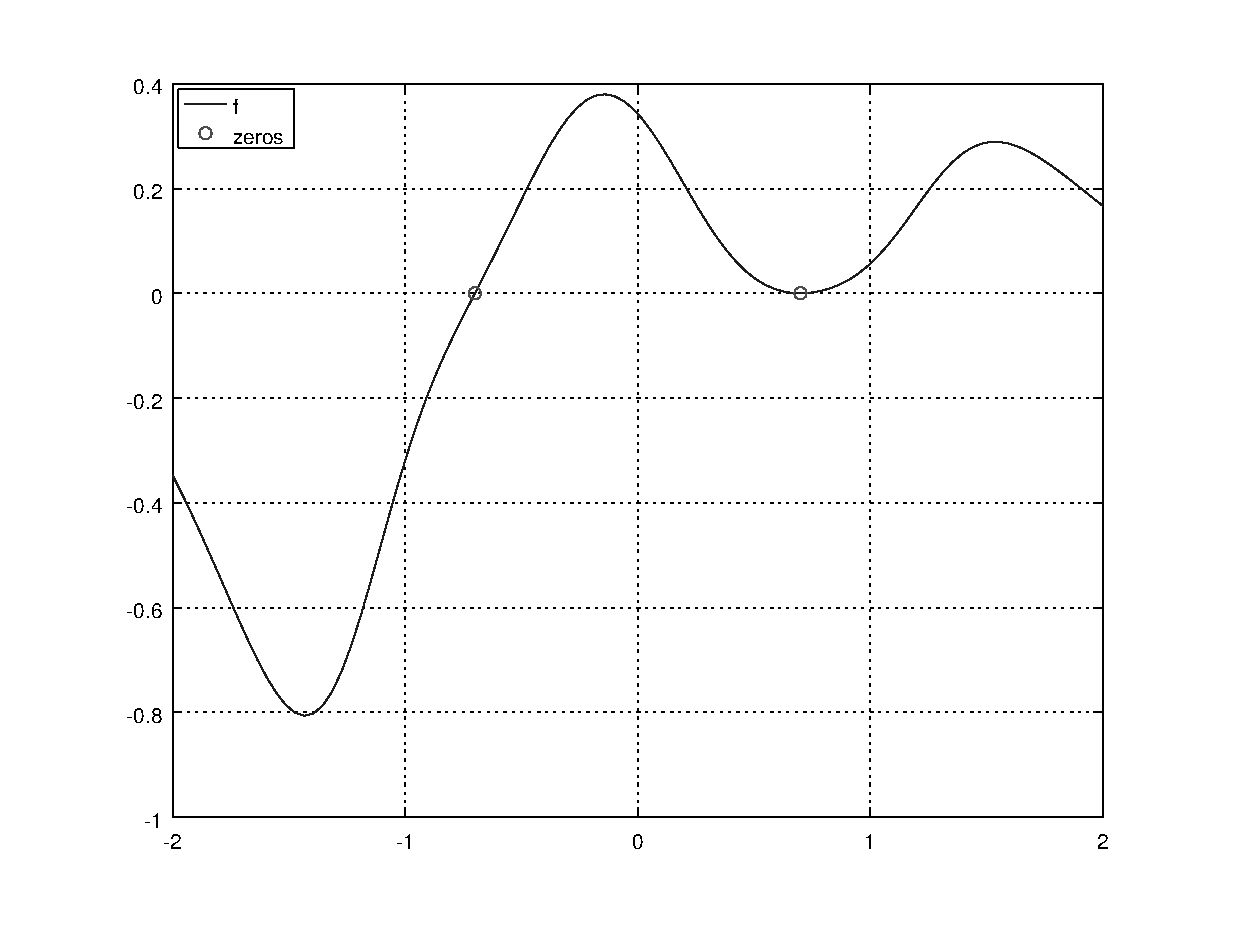
\includegraphics[width=0.8\textwidth]{./cap_eq1d/dados/ex_bis_intro/fig_bis_intro}
  \caption{Esboço da função $f$ do Exemplo~\ref{ex:bis_intro}.}
  \label{fig:bis_intro}
\end{figure}

Observamos que esta função é contínua e que, por exemplo, $f(-2)>0$ e $f(3)<0$, logo $f(-2)\cdot f(3) < 0$ e, de fato, $f$ tem pelo menos um zero\footnote{De fato, $f$ tem três zeros no intervalo $(-2, 3)$.} no intervalo $(-2, 3)$.

\ifisoctave
O esboço do gráfico da função $f$ pode ser feito no \verb+GNU Octave+ com o seguinte \href{https://github.com/phkonzen/notas/blob/master/src/MatematicaNumerica/cap_eq1d/dados/ex_bis_intro/ex_bis_intro.m}{código}:
\verbatiminput{./cap_eq1d/dados/ex_bis_intro/ex_bis_intro.m}
\fi
\end{ex}

Consideremos, então, uma função $f$ contínua tal que $f(a)\cdot f(b) < 0$. O método da bisseção é iterativo, sendo que a primeira aproximação para uma solução de $f(x)=0$ tomada como o ponto médio do intervalo $(a, b)$, i.e.
\begin{equation}
  x^{(1)} = \frac{a^{(1)}+b^{(1)}}{2},
\end{equation}
onde $a^{(1)} = a$ e $b^{(1)} = b$. Daí, se ocorrer $f(x^{(1)})=0$ o problema está resolvido. Caso contrário, $f$ tem pelo menos um zero num dos subintervalos $(a^{(1)}, x^{(1)})$ ou $(x^{(1)}, b^{(1)})$, pois $f(a^{(1)})\cdot f(x^{(1)}) < 0$ ou  $f(x^{(1)})\cdot f(b^{(1)}) < 0$, respectivamente e exclusivamente. No primeiro caso, escolhemos $(a^{(2)}, b^{(2)}) = (a^{(1)}, x^{(1)})$ ou, no segundo caso, tomamos $(a^{(2)}, b^{(2)}) = (x^{(1)}, b^{(1)})$. Então, a segunda aproximação para uma solução é computada como
\begin{equation}
  x^{(2)} = \frac{a^{(2)} + b^{(2)}}{2}.
\end{equation}
Daí, o procedimento se repete até obtermos uma aproximação com a precisão desejada.

\begin{ex}\label{ex:bis_exec}
  Consideremos o problema de encontrar um zero da função
\begin{equation}
  f(x) = \sen^2\left(x+\frac{\pi}{4}\right) - x^3 + \frac{\pi}{4}x^2 + \frac{5\pi^2}{16}x + \frac{3\pi^3}{64}.
\end{equation}
Do esboço de seu gráfico (Figura \ref{fig:bis_intro}) vemos que $f(2)\cdot f(3) \neq 0$ sendo que o zero $x=3\pi/4\approx 2,3562$ de $f$ está no intervalo $(2, 3)$. Então, aplicando o método da bisseção com intervalo inicial $(a^{(1)}, b^{(1)}) = (2, 3)$ e aproximação inicial $x^{(1}) = (a^{(1)}+b^{(1)})/2$, obtemos as aproximações apresentadas na Tabela \ref{tab:bis_exec}.

\begin{table}[h!]
  \centering
  \caption{Resultados referentes ao Exemplo~\ref{ex:bis_exec}.}
  \begin{tabular}{r|rr|r|c}
    k & $a^{(k)}$ & $b^{(k)}$ & $x^{(k)}$ & $f(a^{(k)})\cdot f(x^{(k)})$\\\hline
    1 & $2,0000$ & $3,0000$ & $2,5000$ & -1 \\
    2 & $2,0000$ & $2,5000$ & $2,2500$ &  1 \\
    3 & $2,2500$ & $2,5000$ & $2,3750$ & -1 \\
    4 & $2,2500$ & $2,3750$ & $2,3125$ & 1 \\
    5 & $2,3125$ & $2,3750$ & $2,3438$ & 1 \\
    6 & $2,3438$ & $2,3750$ & $2,3594$ &  -1 \\
    7 & $2,3438$ & $2,3594$ & $2,3516$ & 1 \\
    8 & $2,3516$ & $2,3594$ & $2,3555$ &  1 \\
    9 & $2,3555$ & $2,3594$ & $2,3574$ &  -1 \\
    10 & $2,3555$ & $2,3574$ & $2,3564$ & -1 \\\hline
  \end{tabular}
  \label{tab:bis_exec}
\end{table}

\ifisoctave
A tabela \ref{tab:bis_exec} pode ser obtida no \verb+GNU Octave+ com o seguinte \href{https://github.com/phkonzen/notas/blob/master/src/MatematicaNumerica/cap_eq1d/dados/ex_bis_exec/ex_bis_exec.m}{código}:
\verbatiminput{./cap_eq1d/dados/ex_bis_exec/ex_bis_exec.m}
\fi
\end{ex}

\subsection{Análise de convergência}

Dada uma função estritamente monótona\footnote{Estritamente crescente ou estritamente decrescente.} e contínua $f:[a, b]\to\mathbb{R}$ com $f(a)\cdot f(b) < 0$, temos que o método da bisseção converge para o zero de $f$ no intervalo $(a, b)$. 

De fato, como consequência imediata do \href{https://phkonzen.github.io/notas/AnaliseMatematicaI/cap_continuidade_sec_prop_f_cont.html}{teorema do valor intermediário}, temos que $f$ tem pelo menos um zero no intervalo $(a, b)$. Agora, da hipótese de monotonicidade estrita, temos que $f$ tem um único zero neste intervalo, o qual denotaremos por $x^{*}$.

Da construção das iteradas do método, temos
\begin{align}
  |x^{(k)} - x^{*}| &\leq \frac{b^{(k)}-a^{(k)}}{2}\\
  &\leq \frac{b^{(k-1)}-a^{(k-1)}}{2^2}\\
  &\vdots \\
  &\leq \frac{b^{(1)}-a^{(1)}}{2^k},
\end{align}
donde, temos a seguinte estimativa do erro de truncamento
\begin{equation}\label{eq:bis_est_trunc}
  |x^{(k)} - x^{*}| \leq \frac{b^{(1)}-a^{(1)}}{2^k}.
\end{equation}
E, daí também, segue a convergência do método da bisseção, pois
\begin{equation}
  \lim_{k\to\infty} |x^{(k)}-x^{*}| = \lim_{k\to\infty} \frac{b^{(1)}-a^{(1)}}{2^k} = 0.
\end{equation}

\begin{obs}
  No caso de $f$ não ser estritamente monótona no intervalo $(a, b)$, ainda podemos garantir a convergência do método da bisseção. Isto segue do fato de que após algumas iteradas, digamos $k$ iteradas, a função $f$ terá apenas um zero no intervalo $(a^{(k)}, b^{(k)})$. A partir daí, as estimativas acima podem ser aplicadas.
\end{obs}

\begin{ex}\label{ex:bis_conv}
  No Exemplo \ref{ex:bis_exec} aplicamos o método da bisseção para a função
\begin{equation}
  f(x) = \sen^2\left(x+\frac{\pi}{4}\right) - x^3 + \frac{\pi}{4}x^2 + \frac{5\pi^2}{16}x + \frac{3\pi^3}{64}.
\end{equation}
no intervalo $(2, 3)$. Observando os resultados mostrados na Tabela \ref{tab:bis_exec}, vemos que
\begin{equation}
  |x^{(10)}-x^*| = 2,5\E-4,
\end{equation}
com $x^* = x_1 = 3\pi/4$. Observamos que este resultado é consistente com a estimativa do erro de truncamento \eqref{eq:bis_est_trunc}, da qual temos
\begin{align}
  |x^{(10)} - x^*| &\leq \frac{b^{(1)}-a^{(1)}}{2^{10}}\\
  &= \frac{1}{2^{10}} = 9,8\E-4.
\end{align}
\end{ex}

\begin{obs}(\normalfont{Taxa de convergência.})
  A estimativa de convergência \eqref{eq:bis_est_trunc} também pode ser usada para mostrarmos que, assintoticamente, o método da bisseção tem a seguinte taxa de convergência linear
  \begin{equation}
    \left|x^{(k+1)} - x^{(k)}\right| \lesssim \frac{1}{2}\left|x^{(k)} - x^{(k-1)}\right|^{\pmb{1}}.
  \end{equation}
\end{obs}

\subsection{Zeros múltiplos}

Sejam $f$ uma função suave e $x^*$ um zero de multiplicidade par de $f$. Observamos que o método da bisseção não é diretamente aplicável para aproximar $x^*$. Isto ocorre, pois, neste caso, $x^*$ será um ponto de mínimo ou de máximo local de $f$, não havendo pontos $a$ e $b$ próximos de $x^*$ tal que $f(a)\cdot f(b) < 0$.

Agora, sendo $x^*$ é um zero de multiplicidade $2m$ de $f$, temos que ela admite a seguinte decomposição
\begin{equation}
  f(x) = (x-x^*)^{2m}g(x),
\end{equation}
onde $g$ é uma função suave e $g(x^*)\neq 0$. Daí, a derivada de $f$
\begin{equation}
  f'(x) = 2m(x-x^*)^{2m-1}g(x) + (x-x^*)^{2m}g'(x),
\end{equation}
tem $x^*$ como um zero de multiplicidade $2m-1$ (ímpar) e, desta forma, podemos aplicar o método da bisseção em $f'$ para aproximar $x^*$.

\begin{ex}\label{ex:bis_multpar}
  A função
\begin{equation}
  f(x) = \sen^2\left(x+\frac{\pi}{4}\right) - x^3 + \frac{\pi}{4}x^2 + \frac{5\pi^2}{16}x + \frac{3\pi^3}{64}.
\end{equation}
tem $x=-\pi/4\approx -0,7854$ como um zero de multiplicidade par (veja Figura \ref{fig:bis_intro}). Para aplicarmos o método da bisseção para aproximarmos este zero, primeiramente, derivamos $f$
\begin{equation}
  f'(x) = 2\sin(x+\pi/4)\cos(x+\pi/4) - 3x^2 + \frac{\pi}{2}x + \frac{5\pi^2}{16}.
\end{equation}
O esboço do gráfico de $f'$ (Figura \ref{fig:bis_multpar}) mostra que $f'(-1)\cdot f'(0) < 0$ sendo que no intervalo $(-1, 0)$ $f'$ tem um zero de multiplicidade ímpar. Então, aplicando o método da bisseção a $f'$ no intervalo inicial $(a^{(1)}, b^{(1)}) = (-1, ~0)$, obtemos os resultados apresentados na Tabela~\ref{tab:bis_multpar}. Nesta tabela são apresentados as iteradas até a convergência da solução com precisão de $10^{-3}$.

\begin{figure}[h!]
  \centering
  \includegraphics[width=0.8\textwidth]{./cap_eq1d/dados/ex_bis_multpar/fig_bis_multpar}
  \caption{Esboço do gráfico da $f$ e de sua derivada $f'$ dada no Exemplo \ref{ex:bis_multpar}.}
  \label{fig:bis_multpar}
\end{figure}

\begin{table}[h!]
  \centering
  \caption{Resultados referentes ao Exemplo~\ref{ex:bis_exec}.}
  \begin{tabular}{r|rr|r|c}
    k & $a^{(k)}$ & $b^{(k)}$ & $x^{(k)}$ & $f'(a^{(k)})\cdot f'(x^{(k)})$\\\hline
    1 & $-1,0000\E+0$ & $0,0000\E+0$ & $-5,0000\E-1$ & -1 \\
    2 & $-1,0000\E+0$ & $-5,0000\E-1$ & $-7,5000\E-1$ & -1 \\
    3 & $-1,0000\E+0$ & $-7,5000\E-1$ & $-8,7500\E-1$ & 1 \\
    4 & $-8,7500\E-1$ & $-7,5000\E-1$ & $-8,1250\E-1$ &  1 \\
    5 & $-8,1250\E-1$ & $-7,5000\E-1$ & $-7,8125\E-1$ & -1 \\
    6 & $-8,1250\E-1$ & $-7,8125\E-1$ & $-7,9688\E-1$ & 1 \\
    7 & $-7,9688\E-1$ & $-7,8125\E-1$ & $-7,8906\E-1$ & 1 \\
    8 & $-7,8906\E-1$ & $-7,8125\E-1$ & $-7,8516\E-1$ & -1 \\
    9 & $-7,8906\E-1$ & $-7,8516\E-1$ & $-7,8711\E-1$ & 1 \\
    10 & $-7,8711\E-1$ & $-7,8516\E-1$ & $-7,8613\E-1$ & 1 \\\hline
  \end{tabular}
  \label{tab:bis_multpar}
\end{table}

\ifisoctave
A tabela \ref{tab:bis_multpar} pode ser obtida no \verb+GNU Octave+ com o seguinte \href{https://github.com/phkonzen/notas/blob/master/src/MatematicaNumerica/cap_eq1d/dados/ex_bis_multpar/ex_bis_multpar.m}{código}:
\verbatiminput{./cap_eq1d/dados/ex_bis_multpar/ex_bis_multpar.m}
\fi
\end{ex}

\subsection*{Exercícios}

\begin{exer}\label{exer:bis_1}
  Use o método da bisseção para aproximar um zero de $f(x)=x^3\sen(x)-\cos(x)$, aplicando como intervalo inicial $(a^{(1)}, b^{(1)}) = (0,5, ~1)$ e aproximação inicial $x^{(1)}=(a^{(1)}+b^{(1)})/2$. Faça, então, $6$ iterações de forma a obter a aproximação $x^{(7)}$ e forneça-a com $7$ dígitos significativos por arredondamento.
\end{exer}
\begin{resp}
    \ifisoctave 
  \href{https://github.com/phkonzen/notas/blob/master/src/MatematicaNumerica/cap_eq1d/dados/exer_bis_1/exer_bis_1.m}{Código.} 
  \fi
  $9,179688\times 10^{-1}$
\end{resp}

\begin{exer}\label{exer:bis_est_trunc}
  Considere que o método da bisseção para aproximar um zero de $f(x)=x^3\sen(x)-\cos(x)$, aplicando como intervalo inicial $(a^{(1)}, b^{(1)}) = (0,5, ~1)$ e aproximação inicial $x^{(1)}=(a^{(1)}+b^{(1)})/2$. Use a estimativa de convergência \eqref{eq:bis_est_trunc}
  \begin{equation}
    \left|x^{(k)} - x^{*}\right| \leq \frac{b^{(1)}-a^{(1)}}{2^k},
  \end{equation}
para estimar o número mínimo de iterações $k_{conv}$ necessárias para se obter a solução com exatidão de $10^{-4}$. Então, compute $x^{(k_{conv})}$ e forneça-o com $6$ dígitos significativos por arredondamento.
\end{exer}
\begin{resp}
    \ifisoctave 
  \href{https://github.com/phkonzen/notas/blob/master/src/MatematicaNumerica/cap_eq1d/dados/exer_bis_este_trunc/exer_bis_est_trunc.m}{Código.} 
  \fi
  $9,15833\E-1$
\end{resp}

\begin{exer}\label{exer:bis_multpar}
  Use o método da bisseção para encontrar uma aproximação com precisão de $10^{-4}$ do zero de
  \begin{equation}
    f(x) = (-x^2+1,154x-0,332929)\cos(x) + x^2 - 1,154x + 0,332929
  \end{equation}
no intervalo $(0,55, ~0,65)$. Forneça a aproximação computada com $7$ dígitos significativos por arredondamento.
\end{exer}
\begin{resp}
    \ifisoctave 
  \href{https://github.com/phkonzen/notas/blob/master/src/MatematicaNumerica/cap_eq1d/dados/exer_bis_multpar/exer_bis_multpar.m}{Código.} 
  \fi
  $5,770508\times 10^{-1}$
\end{resp}

\section{Método da falsa posição}\label{cap_eq1d_sec_falsapos}

O método da falsa posição é uma variação do método da bisseção. Dada uma função $f$ contínua, escolhemos um intervalo inicial $(a, b)$ tal que $f(a)\cdot f(b) < 0$ (i.e. $f$ tem sinais trocados nos pontos $a$ e $b$). Então, uma aproximação para o zero de $f$ neste intervalo é computada como o ponto de interseção da reta secante a $f$ pelos pontos $(a, f(a))$ e $(b, f(b))$, i.e.
\begin{equation}
  x = a - \frac{b-a}{f(b)-f(a)}f(a).
\end{equation}
Veja a Figura \ref{fig:falsapos}.

\begin{figure}[h!]
  \centering
  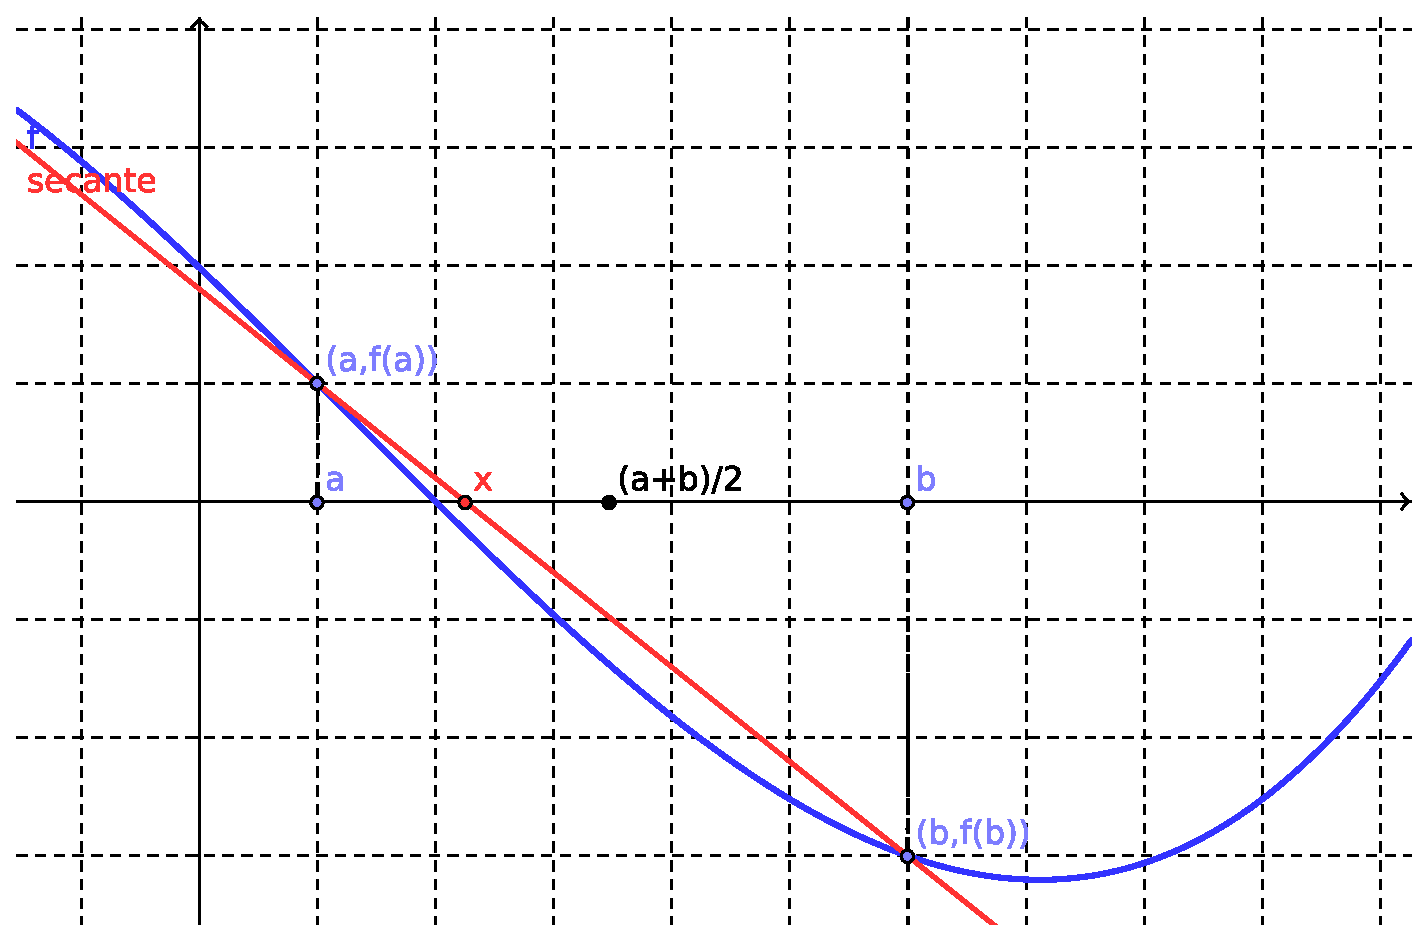
\includegraphics[width=0.7\textwidth]{./cap_eq1d/dados/fig_falsapos/fig_falsapos}
  \caption{Ilustração do método da falsa posição (veja no \href{https://github.com/phkonzen/notas/blob/master/src/MatematicaNumerica/cap_eq1d/dados/fig_falsapos/fig_falsapos.ggb}{Geogebra}).}
  \label{fig:falsapos}
\end{figure}

Mais explicitamente, o método da falsa posição consiste no seguinte procedimento iterativo:
\begin{enumerate}
\item Determinar um intervalo $(a^{(1)}, b^{(1)})$ tal que $f(a^{(1)})\cdot f(b^{(1)}) \neq 0$.
\item Para $k = 1, 2, 3, \cdots, N$:
  \begin{enumerate}[2.1]
  \item $\displaystyle x^{(k)} = a^{(k)} - \frac{b^{(k)}-a^{(k)}}{f(b^{(k)})-f(a^{(k)})}f(a^{(k)})$
  \item Verificar critério de parada.
  \item Se $f(a^{(k)})\cdot f(x^{(k)}) \neq 0$, então $a^{(k+1)}=a^{(k)}$ e $b^{(k+1)}=x^{(k)}$.
  \item Se $f(x^{(k)})\cdot f(b^{(k)}) \neq 0$, então $a^{(k+1)}=x^{(k)}$ e $b^{(k+1)}=b^{(k)}$.
  \end{enumerate}
\end{enumerate}

\begin{ex}\label{ex:falsapos_exec}
  Consideremos o problema de aproximar o zero de
\begin{equation}
  f(x) = \sen^2\left(x+\frac{\pi}{4}\right) - x^3 + \frac{\pi}{4}x^2 + \frac{5\pi^2}{16}x + \frac{3\pi^3}{64}.
\end{equation}
no intervalo $(0, 3)$. A Tabela \ref{tab:falsapos_exec} mostra os resultados obtidos da aplicação do método da falsa posição com intervalo inicial $(a^{(1)}, b^{(1)}) = (2, 3)$. Aqui, o método foi iterado até a convergência com cinco dígitos significativos.

\begin{table}[h!]
  \centering
  \caption{Resultados referentes ao Exemplo~\ref{ex:falsapos_exec}.}
  \begin{tabular}{r|rr|r|c}
    k & $a^{(k)}$ & $b^{(k)}$ & $x^{(k)}$ & $f'(a^{(k)})\cdot f'(x^{(k)})$\\\hline
    1 & $2,0000$ & $3,0000$ & $2,2455$ & 1 \\
    2 & $2,2455$ & $3,0000$ & $2,3240$ &  1 \\
    3 & $2,3240$ & $3,0000$ & $2,3470$ & 1 \\
    4 & $2,3470$ & $3,0000$ & $2,3536$ & 1 \\
    5 & $2,3536$ & $3,0000$ & $2,3555$ & 1 \\
    6 & $2,3555$ & $3,0000$ & $2,3560$ & 1 \\
    7 & $2,3560$ & $3,0000$ & $2,3561$ &  1 \\
    8 & $2,3561$ & $3,0000$ & $2,3562$ & 1 \\
    9 & $2,3562$ & $3,0000$ & $2,3562$ & 1 \\
    10 & $2,3562$ & $3,0000$ & $2,3562$ & 1 \\\hline
  \end{tabular}
  \label{tab:falsapos_exec}
\end{table}

\ifisoctave
A tabela \ref{tab:falsapos_exec} pode ser obtida no \verb+GNU Octave+ com o seguinte \href{https://github.com/phkonzen/notas/blob/master/src/MatematicaNumerica/cap_eq1d/dados/ex_falsapos_exec/ex_falsapos_exec.m}{código}:
\verbatiminput{./cap_eq1d/dados/ex_falsapos_exec/ex_falsapos_exec.m}
\fi
\end{ex}

\subsection*{Exercícios}

\begin{exer}\label{exer:falsapos_1}
  Use o método da falsa posição para aproximar um zero de $f(x)=x^3\sen(x)-\cos(x)$, aplicando como intervalo inicial $(a^{(1)}, b^{(1)}) = (0,5, ~1)$ e aproximação inicial
  \begin{equation}
    x^{(1)} = a^{(1)} - \frac{b^{(1)}-a^{(1)}}{f(b^{(1)})-f(a^{(1)})}f(a^{(1)}).
  \end{equation}
Faça, então, $4$ iterações deste método de forma a obter a aproximação $x^{(5)}$ e forneça-a com $7$ dígitos significativos por arredondamento.
\end{exer}
\begin{resp}
    \ifisoctave 
  \href{https://github.com/phkonzen/notas/blob/master/src/MatematicaNumerica/cap_eq1d/dados/exer_falsapos_1/exer_falsapos_1.m}{Código.} 
  \fi
  $9,158079\times 10^{-1}$
\end{resp}

\begin{exer}\label{exer:falsapos_multpar}
  Use o método da bisseção para encontrar uma aproximação com precisão de $10^{-4}$ do zero de
  \begin{equation}
    f(x) = (-x^2+1,154x-0,332929)\cos(x) + x^2 - 1,154x + 0,332929
  \end{equation}
no intervalo $(0,55, ~0,65)$. Forneça a aproximação computada com $7$ dígitos significativos por arredondamento.
\end{exer}
\begin{resp}
    \ifisoctave 
  \href{https://github.com/phkonzen/notas/blob/master/src/MatematicaNumerica/cap_eq1d/dados/exer_falsapos_multpar/exer_falsapos_multpar.m}{Código.} 
  \fi
  $5,76984\times 10^{-1}$
\end{resp}

\section{Iteração de ponto fixo}\label{cap_eq1d_pfixo}

O ponto fixo de uma função dada $g$ é o ponto $x$ tal que
\begin{equation}
  g(x) = x.
\end{equation}
Geometricamente, pontos fixos são interseções do gráfico da $g$ com a reta $y=x$, veja a Figura \ref{fig:pfixo}.

\begin{figure}[h!]
  \centering
  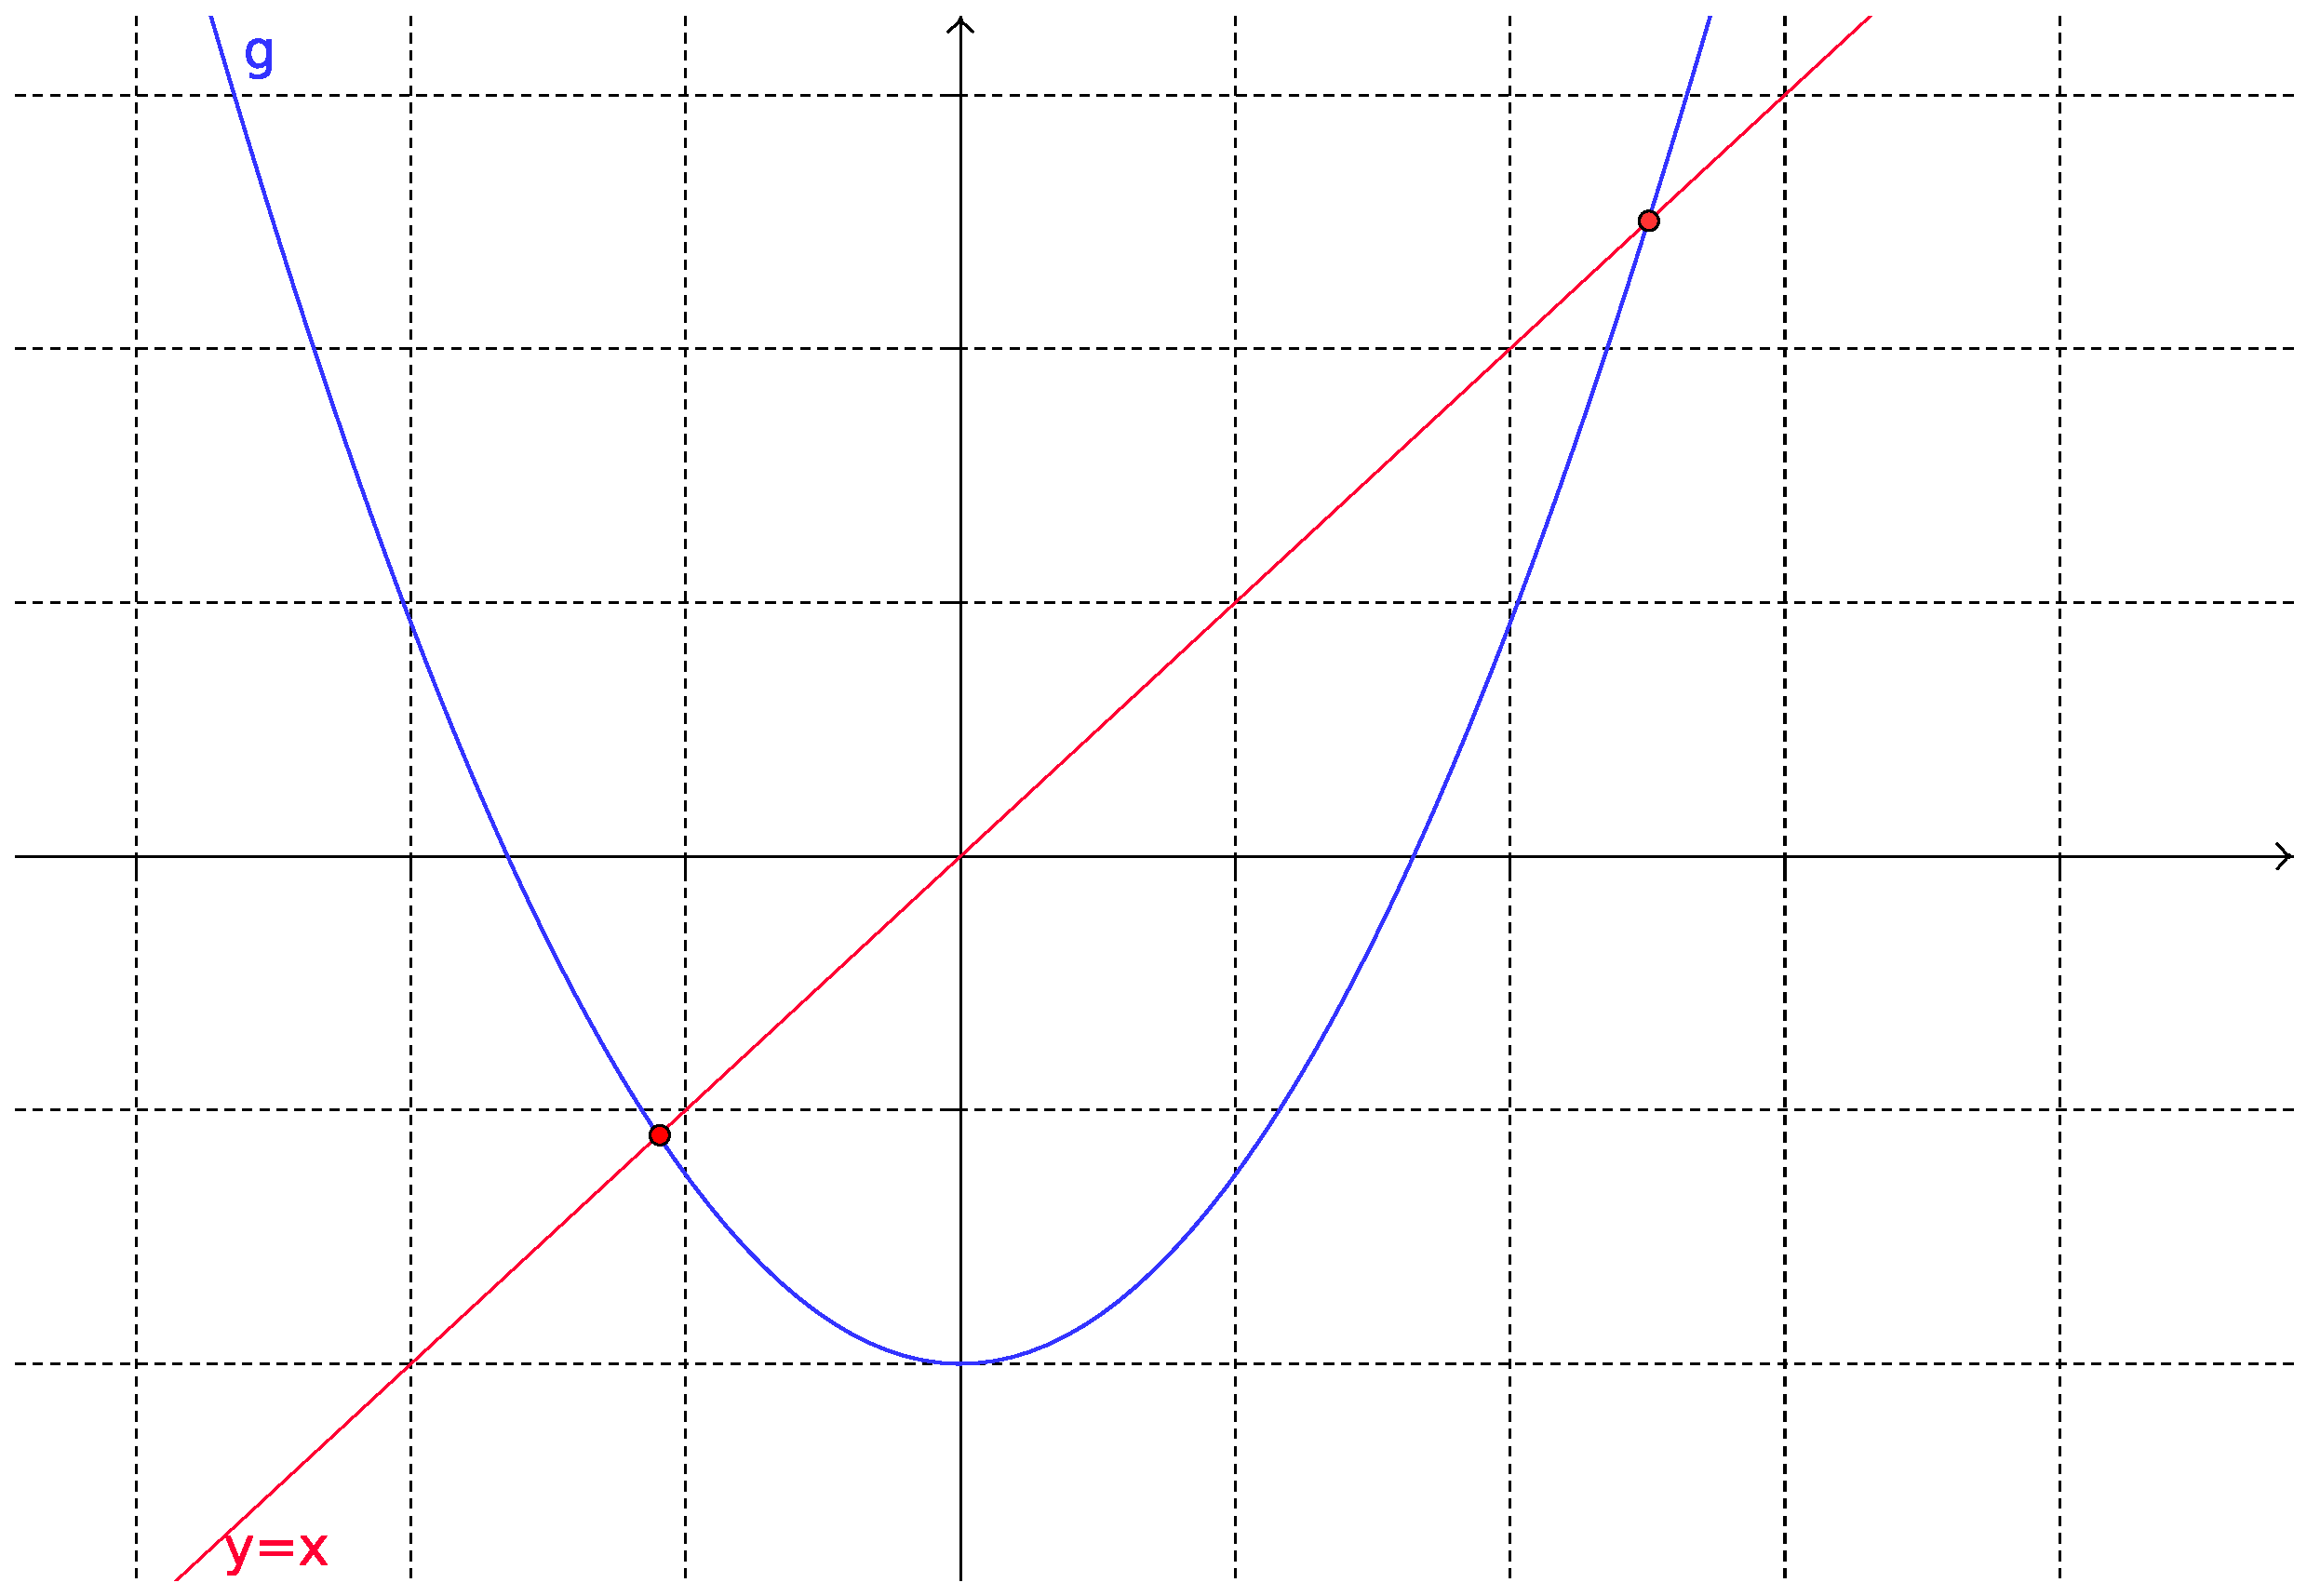
\includegraphics[width=0.8\textwidth]{./cap_eq1d/dados/fig_pfixo/fig_pfixo}
  \caption{Exemplos de pontos fixos (veja no \href{https://github.com/phkonzen/notas/blob/master/src/MatematicaNumerica/cap_eq1d/dados/fig_pfixo/fig_pfixo.ggb}{Geogebra}).}
  \label{fig:pfixo}
\end{figure}

Observamos que toda equação de uma incógnita pode ser reescrita de forma equivalente como um problema de ponto fixo.

\begin{ex}\label{ex:pfixo_intro}
  Consideremos o problema de resolver
  \begin{equation}
    \sen^2\left(x+\frac{\pi}{4}\right) = x^3 - \frac{\pi}{4}x^2 - \frac{5\pi^2}{16}x - \frac{3\pi^3}{64}.
  \end{equation}
Podemos reescrevê-la como o problema de se obter os zeros da seguinte função
\begin{equation}
  f(x) = \sen^2\left(x+\frac{\pi}{4}\right) - x^3 + \frac{\pi}{4}x^2 + \frac{5\pi^2}{16}x + \frac{3\pi^3}{64}.
\end{equation}
Por sua vez, este problema é equivalente aos seguintes problemas de ponto fixo (entre outros):
\begin{align}
  &a)~g_1(x) = \frac{16}{5\pi^2}\left[-\sen^2\left(x+\frac{\pi}{4}\right) + x^3 - \frac{\pi}{4}x^2 - \frac{3\pi^3}{64}\right] = x.\\
  &b)~g_2(x) = \sqrt[3]{\sen^2\left(x+\frac{\pi}{4}\right) + \frac{\pi}{4}x^2 + \frac{5\pi^2}{16}x + \frac{3\pi^3}{64}}
\end{align}
Na Figura \ref{fig:pfixo_intro} podemos observar que os zeros da $f$ (a saber, $x_1=3\pi/4\approx 2,3562$ e $x_2=x_3=-\pi/4\approx -0,78540$) coincidem com os pontos fixos das funções $g_1$ e $g_2$.

\begin{figure}[h!]
  \centering
  \includegraphics[width=0.8\textwidth]{./cap_eq1d/dados/ex_pfixo_intro/fig_pfixo_intro}
  \caption{Esboço da função $f$ do Exemplo~\ref{ex:pfixo_intro}.}
  \label{fig:pfixo_intro}
\end{figure}
\end{ex}

Em muitos casos, é possível obter aproximações de um ponto fixo de uma dada função $g$ pela chamada \emph{iteração de ponto fixo}:
\begin{align}
  x^{(1)} &= \text{aprox. inicial}\\
  x^{(k+1)} &= g(x^{(k)}),\quad k=1, 2, 3, \ldots
\end{align}

\begin{ex}\label{ex:pfixo_testes}
  Observemos que para a função $g_1$ dada no Exemplo \ref{ex:pfixo_intro}, temos as seguintes iterações:
  \begin{align}
    x^{(1)} &= -0,70000,\\
    x^{(2)} &= -0,70959,\\
    x^{(3)} &= -0,71716,\\
    &\vdots \\
    x^{(100)} &= -0,77862,\\
    &\vdots \\
    x^{(1000)} &= -0,78466,\\    
    &\vdots \\
    x^{(20000)} &= -0,78536.
  \end{align}
Ou seja, neste caso as iterações de ponto fixo convergem (lentamente) para o ponto fixo $x=-\pi/4\approx -0,78540$.
\ifisoctave
Veja o \href{https://github.com/phkonzen/notas/blob/master/src/MatematicaNumerica/cap_eq1d/dados/ex_pfixo_testes/ex_g1_t1.m}{código} no \verb+GNU Octave+.
\fi

Agora, se usarmos a iteração de ponto fixo com esta mesma função para aproximar o ponto fixo $x=3\pi/4\approx 2,3562$, obtemos
  \begin{align}
    x^{(1)} &= 2,50000,\\
    x^{(2)} &= 2,9966,\\
    x^{(3)} &= 5,8509,\\
    &\vdots \\
    x^{(8)} &= 4,8921e\times 10^{121}.
  \end{align}
Donde observamos que as iterações divergem rapidamente.

Entretanto, se usarmos a iteração de ponto fixo com a função $f_2$ dada no Exemplo \ref{ex:pfixo_intro}, obtemos
  \begin{align}
    x^{(1)} &= 2,50000,\\
    x^{(2)} &= 2,4155,\\
    x^{(3)} &= 2,3805,\\
    &\vdots \\
    x^{(10)} &= 2,3562.
  \end{align}
A qual, portanto, converge para o ponto fixo esperado.
\end{ex}

Este último exemplo (Exemplo \ref{ex:pfixo_testes}) mostra que a iteração do ponto fixo nem sempre é convergente. Antes de vermos condições suficientes para a convergência, vejamos sua interpretação geométrica.

\subsection{Interpretação geométrica}

A Figura \ref{fig:pfixo_interp} apresenta o caso de uma iteração de ponto fixo convergente. As iterações iniciam-se no ponto $x^{(1)}$ e seguem para $x^{(2)} = g(x^{(1)})$ e $x^{(3)} = g(x^{(2)})$.

\begin{figure}[h!]
  \centering
  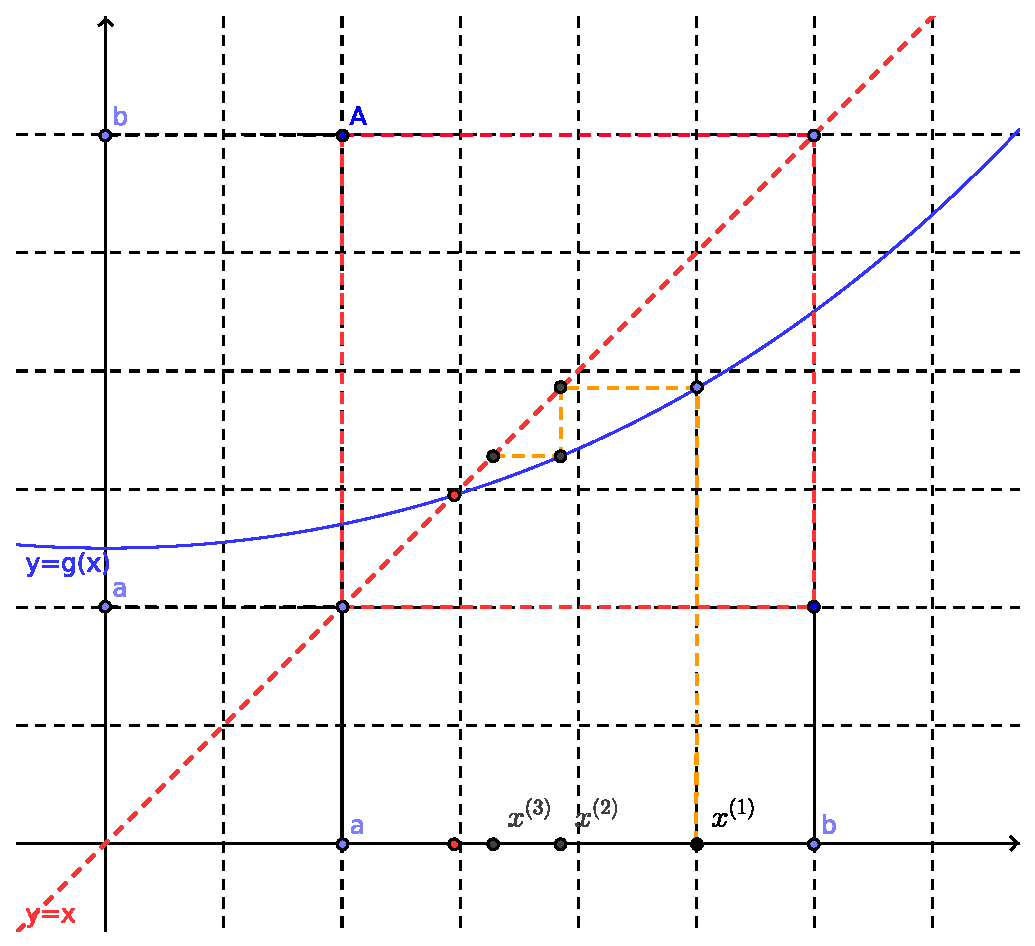
\includegraphics[width=0.8\textwidth]{./cap_eq1d/dados/fig_pfixo_interp/fig_pfixo_interp}
  \caption{Interpretação geométrica da iteração de ponto fixo.}
  \label{fig:pfixo_interp}
\end{figure}

\subsection{Análise de convergência}

O seguinte teorema nos fornece condições suficientes para a convergência das iterações de ponto fixo.

\begin{teo}(\normalfont{Teorema do ponto fixo})\label{teo:pfixo}
  Seja uma dada função $g$ continuamente diferenciável satisfazendo
  \begin{enumerate}[a)]
  \item $g([a, b]) \subset [a, b]$,
  \item $|g'(x)|<K<1$ para todo $x\in [a, b]$.
  \end{enumerate}
Então, $g$ tem um único ponto fixo $x^*\in [a, b]$ e as iterações $x^{(k+1)}=x^{(k)}$, $k=1, 2, 3, \ldots$, convergem para $x^*$, para qualquer escolha de $x^{(1)}\in [a, b]$.
\end{teo}
\begin{dem}
  Da hipótese b), temos que $g$ é uma contração com
  \begin{equation}
    |g(x) - g(y)| < K\cdot |x - y|,~\forall x,y\in [a, b].
  \end{equation}
Com isso, da hipótese a) e tomando $x^{(1)}\in [a, b]$, temos
\begin{align}
  |x^{(k+1)} - x^{(k)}| &= |g(x^{(k)}) - g(x^{(k-1)})|\\
  &\leq K |x^{(k)} - x^{(k-1)}|\\
  &\vdots \\
  &\leq K^{k-1}|x^{(2)}-x^{(1)}|,
\end{align}
para todo $k=2, 3, \ldots$. Como $K<1$, temos $|x^{(k+1)}-x^{(k)}|\to 0$ quando $k\to\infty$ e, portanto, $x^{(k)}$ converge para algum $x^*\in [a, b]$.

De fato, $x^*$ é ponto fixo de $g$, pois da continuidade da $g$, temos
\begin{equation}
  x^* = \lim_{k\to\infty} x^{(k+1)} = \lim_{k\to\infty} g(x^{(k)}) = g(x^*).
\end{equation}

Por fim, $x^*$ é único, pois assumindo a existência de outro ponto fixo $x^{**}\neq x^*$ teríamos
\begin{equation}
  |x^* - x^{**}| = |g(x^*) - g(x^{**})| < K|x^* - x^{**}|.
\end{equation}
\end{dem}

Agora, dado um problema de encontrar um zero de uma dada função $f$, i.e. $f(x)=0$, podemos construir uma função $g$ para a iteração de ponto fixo associada da seguinte forma:
\begin{align}
  f(x) = 0 &\Leftrightarrow \underbrace{x - \alpha f(x)}_{g(x)} = x,
\end{align}
com $\alpha\in\mathbb{R}$ escolhido de forma a satisfazer as hipóteses do teorema do ponto fixo (Teorema \ref{teo:pfixo}).

\begin{ex}\label{ex:pfixo_exec}
  Retornamos ao problema de encontrar o zero da função
  \begin{equation}
    f(x) = \sen^2\left(x+\frac{\pi}{4}\right) - x^3 + \frac{\pi}{4}x^2 + \frac{5\pi^2}{16}x + \frac{3\pi^3}{64}.
  \end{equation}
  no intervalo $[2,3]$. Para construir uma função $g$ para a iteração de ponto fixo neste intervalo, podemos tomar
  \begin{equation}
    g(x) = x - \alpha f(x),
  \end{equation}
com $\alpha = -0,1$. A Figura \ref{fig:ex_pfixo_exec} mostra esboços dos gráficos de $g$ e $|g'|$ no intervalos $[2, 3]$ e podemos observar que esta escolha de $\alpha$ faz com que a $g$ satisfaça o teorema do ponto fixo.

\begin{figure}[h!]
  \centering
  \includegraphics[width=0.8\textwidth]{./cap_eq1d/dados/ex_pfixo_exec/fig_ex_pfixo_exec}
  \caption{Esboço dos gráficos de $g$ e $|g'|$ discutidas no Exemplo \ref{ex:pfixo_exec}.}
  \label{fig:ex_pfixo_exec}
\end{figure}

Então, fazendo as iterações de ponto fixo com aproximação inicial $x^{(1)}=2,6$, obtemos os resultados apresentados na Tabela \ref{tab:ex_pfixo_exec}.

\begin{table}[h!]
  \centering
  \begin{tabular}{r|cc}
    $k$ & $x^{(k)}$ & $|x^{(k)}-x^{(k-1)}|$ \\\hline
    1 & $2,6000$ & -x-\\
    2 & $2,3264$ & $2,7\E-1$ \\
    3 & $2,3553$ & $2,9\E-2$ \\
    4 & $2,3562$ & $8,4\E-4$ \\
    5 & $2,3562$ & $1,1\E-5$ \\\hline
  \end{tabular}
  \caption{Resultados referentes ao Exemplo \ref{ex:pfixo_exec}.}
  \label{tab:ex_pfixo_exec}
\end{table}

\ifisoctave
Os resultados apresentados na Tabela \ref{tab:ex_pfixo_exec} podem ser computados no \verb+GNU Octave+ com o seguinte código:
\verbatiminput{./cap_eq1d/dados/ex_pfixo_exec/ex_pfixo_exec.m}
\fi
\end{ex}

\begin{obs}(\normalfont{Taxa de convergência})
  A iteração de ponto fixo tem taxa de convergência linear
  \begin{equation}
    |x^{(k+1)} - x^{(k)}| < K|x^{(k)} - x^{(k-1)}|^{\pmb{1}},
  \end{equation}
onde $K > 0$ é a constante dada na hipótese $b)$ do teorema do ponto fixo (Teorema \ref{teo:pfixo}). Além disso, isso mostra que quanto menor o valor da constante $K$, mais rápida será a convergência das iterações de ponto fixo.
\end{obs}

\subsection*{Exercícios}

\begin{exer}\label{exer:pfixo_1}
  Considere o problema de computar uma aproximação do zero de $f(x)=x-\cos(x)$. Resolva-o aplicando a iteração de ponto fixo para a função auxiliar
  \begin{equation}
    g(x) = x - \alpha f(x),
  \end{equation}
restrita ao intervalo $[a, b] = [0.5, 1]$ com aproximação inicial $x^{(1)}=(a+b)/2$. Escolha o melhor valor de $\alpha$ entre os seguintes:
\begin{enumerate}
\item $\alpha = 1$
\item $\alpha = 0,5$
\item $\alpha = -0,5$
\item $\alpha = 0,6$
\end{enumerate}
Então, compute uma aproximação do zero de $f$ com $5$ dígitos significativos de precisão.
\end{exer}
\begin{resp}
  \ifisoctave 
  \href{https://github.com/phkonzen/notas/blob/master/src/MatematicaNumerica/cap_eq1d/dados/exer_pfixo_1/exer_pfixo_1.m}{Código.} 
  \fi
  $8,2413\times 10^{-1}$
\end{resp}

\section{Método de Steffensen}\label{cap_eq1d_sec_Steffensen}

O método de Steffensen\footnote{Johan Frederik Steffensen, matemático e estatístico dinamarquês, 1873 - 1961. Fonte: \href{https://en.wikipedia.org/wiki/Johan_Frederik_Steffensen}{Wikipedia}.} é uma aplicação do método de aceleração de convergência $\Delta^2$ de Aitken\footnote{Alexander Aitken, matemático neozelandês, 1895 - 1967. Fonte: \href{https://en.wikipedia.org/wiki/Alexander_Aitken}{Wikipedia}.} à iteração de ponto fixo.

\subsection{Acelerador $\Delta^2$ de Aitken}

Seja dada uma sequência $(x^{(k)})_{k=1}^\infty$ monotonicamente convergente para $x^*$. Assumamos que $k$ seja suficientemente grande tal que
\begin{equation}
  \frac{x^{(k+1)}-x^*}{x^{(k)}-x^*} \approx \frac{x^{(k+2)}-x^*}{x^{(k+1)}-x^*}.
\end{equation}
Então, isolando $x^*$ obtemos
\begin{equation}
  x^* \approx \frac{x^{(k)}x^{(k+2)}-(x^{(k+1)})^2}{x^{(k)}-2x^{(k+1)}+x^{(k+2)}}.
\end{equation}
Ainda, somando e subtraindo $(x^{(k)})^2$ e $2x^{(k)}x^{(k+1)}$ no numerador acima e rearranjando os termos, obtemos
\begin{equation}
  x^* \approx x^{(k)} - \frac{(x^{(k+1)}-x^{(k)})^2}{x^{(k+2)}-2x^{(k+1)}+x^{(k)}}.
\end{equation}

O observado acima, nos motiva a introduzir o acelerador $\Delta^2$ de Aitken
\begin{equation}
  \Delta^2\{x^{(k)},x^{(k+1)},x^{(k+2)}\} := x^{(k)} - \frac{(x^{(k+1)}-x^{(k)})^2}{x^{(k+2)}-2x^{(k+1)}+x^{(k)}}.
\end{equation}


\begin{ex}\label{ex:Aitken}
  Consideremos o problema de encontrar o zero da função
  \begin{equation}
    f(x) = \sen^2\left(x+\frac{\pi}{4}\right) - x^3 + \frac{\pi}{4}x^2 + \frac{5\pi^2}{16}x + \frac{3\pi^3}{64}.
  \end{equation}
  no intervalo $[2,3]$. Para tanto, podemos aplicar a iteração de ponto fixo dada por
  \begin{equation}
    x^{(k+1)} = g(x^{(k)}) := x^{(k)} - \alpha f(x^{(k)}),\quad k=1,2,\ldots,
  \end{equation}
com $\alpha=-0,05$ e $x^{(1)}=2,6$. Na Tabela \ref{tab:ex_Aitken} temos os valores das iteradas $x^{(k)}$ e das correções $\Delta^2 = \Delta^2\{x^{(k)},x^{(k+1)},x^{(k+2)}\}$ de Aitken. Neste caso, a aceleração de convergência é notável.

\begin{table}[h!]
  \centering
  \begin{tabular}{r|cc}
    $k$ & $x^{(k)}$ & $\Delta^2$ \\\hline
    1 & $2,6000$ & -x- \\
    2 & $2,4632$ & -x- \\
    3 & $2,4073$ & $2,3687$ \\
    4 & $2,3814$ & $2,3590$ \\
    5 & $2,3688$ & $2,3569$ \\
    6 & $2,3625$ & $2,3564$ \\
    7 & $2,3594$ & $2,3562$ \\
    8 & $2,3578$ & $2,3562$ \\\hline
  \end{tabular}
  \caption{Resultados referentes ao Exemplo \ref{ex:Aitken}.}
  \label{tab:ex_Aitken}
\end{table}

\ifisoctave
Os resultados apresentados na Tabela \ref{tab:ex_Aitken} podem ser computados no \verb+GNU Octave+ com o seguinte \href{https://github.com/phkonzen/notas/blob/master/src/MatematicaNumerica/cap_eq1d/dados/ex_Aitken/ex_Aitken.m}{código}:
\verbatiminput{./cap_eq1d/dados/ex_Aitken/ex_Aitken.m}
\fi
\end{ex}

\subsection{Algoritmo de Steffensen}

O método de Steffensen consiste em aplicar o acelerador $\Delta^2$ de Aitken à iteração de ponto fixo. Mais especificamente, sejam uma aproximação inicial $x^{(1)}$ e uma iteração de ponto fixo
\begin{equation}
  x^{(k+1)} = g(x^{(k)}),\quad k=1,2,\ldots.
\end{equation}
O algoritmo de Steffensen pode ser descrito como segue:
\begin{enumerate}
\item Fazemos $x = x^{(1)}$.
\item Para $k=1,2,3,\dotsc, N-1$:
  \begin{enumerate}
  \item Computamos $x_1 = g(x^{(k)})$.
  \item Computamos $x_2 = g(x_1)$.
  \item Computamos $x^{(k+1)} = \Delta^2\{x^{(k)},x_1,x_2\}$
  \item Verificamos o critério de parada.
  \end{enumerate}
\end{enumerate}


\begin{ex}\label{ex:Steffensen_exec}
  Retornemos ao exemplo anterior (Exemplo \ref{ex:Aitken}. Na Tabela \ref{tab:ex_Steffensen_exec} temos os valores das iteradas de Steffensen $x^{(k)}$ e do indicador de convergência $|x^{(k)}-x^{(k-1)}|$. Observe que os resultados são compatíveis com aqueles obtidos no último exemplo.

\begin{table}[h!]
  \centering
  \begin{tabular}{r|cc}
    $k$ & $x^{(k)}$ & $|x^{(k)}-x^{(k-1)}|$ \\\hline
    1 & $2,6000$ & -x- \\
    2 & $2,3687$ & $2,3\E-1$ \\
    3 & $2.3562$ & $1,2\E-2$ \\
    4 & $2,3562$ & $4,2\E-5$ \\\hline
  \end{tabular}
  \caption{Resultados referentes ao Exemplo \ref{ex:Steffensen_exec}.}
  \label{tab:ex_Steffensen_exec}
\end{table}

\ifisoctave
Os resultados apresentados na Tabela \ref{tab:ex_Steffensen_exec} podem ser computados no \verb+GNU Octave+ com o seguinte \href{https://github.com/phkonzen/notas/blob/master/src/MatematicaNumerica/cap_eq1d/dados/ex_Steffensen_exec/ex_Steffensen_exec.m}{código}:
\verbatiminput{./cap_eq1d/dados/ex_Steffensen_exec/ex_Steffensen_exec.m}
\fi
\end{ex}

\subsection*{Exercícios}

\begin{exer}\label{exer:Steffensen_1}
  Use o método de Steffensen para obter uma aproximação do zero de $f(x)=x^3\sen(x)-\cos(x)$ no intervalo $[0,5, 1]$ com precisão de $10^{-6}$.
\end{exer}
\begin{resp}
    \ifisoctave 
    \href{https://github.com/phkonzen/notas/blob/master/src/MatematicaNumerica/cap_eq1d/dados/exer_Steffensen_1/exer_Steffensen_1.m}{Código.} 
    \fi
    $9,15811\times 10^{-1}$
\end{resp}

\section{Método de Newton}\label{cap_mef1d_sec_newton}

Seja $x^*$ um zero de uma dada função $f$, i.e. $f(x^*)=0$. Usando de expansão em polinômio de Taylor da $f$ em um dado ponto $\tilde{x}$, temos
\begin{equation}
  f(x^*) = f(\tilde{x}) + f'(\tilde{x})(x^*-\tilde{x}) + O((x^*-\tilde{x})^2).
\end{equation}
Como $f(x^*)=0$, temos
\begin{equation}
  x^* + O((x^*-\tilde{x})^2) = \tilde{x} - \frac{f(\tilde{x})}{f'(\tilde{x})}.
\end{equation}
Esta última expressão nos indica que dada uma aproximação $\tilde{x}$ do zero de $f$ a expressão
\begin{equation}
  \tilde{x} - \frac{f(\tilde{x})}{f'(\tilde{x})},
\end{equation}
aproxima $x^*$ com um erro da ordem de $(x^*-\tilde{x})^2$.

Estes observações nos levam a \emph{iteração de Newton}\footnote{Sir Isaac Newton, matemático e físico inglês, 1642 - 1726/27. Fonte: \href{https://en.wikipedia.org/wiki/Isaac_Newton}{Wikipedia}.}\index{iteração de!Newton}
\begin{align}
  x^{(1)} &= \text{aprox. inicial},\\
  x^{(k+1)} &= x^{(k)} - \frac{f(x^{(k)})}{f'(x^{(k)})},\label{eq:Newton_iteracao}
\end{align}
com $k=1, 2, \ldots$.

\begin{ex}\label{ex:Newton_exec}
  Retornamos ao problema de encontrar o zero da função
  \begin{equation}
    f(x) = \sen^2\left(x+\frac{\pi}{4}\right) - x^3 + \frac{\pi}{4}x^2 + \frac{5\pi^2}{16}x + \frac{3\pi^3}{64}.
  \end{equation}
  no intervalo $[2,3]$. Então, fazendo as iterações de Newton com aproximação inicial $x^{(1)}=2,6$, obtemos os resultados apresentados na Tabela \ref{tab:ex_Newton_exec}.

\begin{table}[h!]
  \centering
  \begin{tabular}{r|cc}
    $k$ & $x^{(k)}$ & $|x^{(k)}-x^{(k-1)}|$ \\\hline
    1 & $2,6000$ & -x-\\
    2 & $2,3836$ & $2,2\E-1$ \\
    3 & $2,3566$ & $2,7\E-2$ \\
    4 & $2,3562$ & $3,9\E-4$ \\
    5 & $2,3562$ & $8,3\E-8$ \\\hline
  \end{tabular}
  \caption{Resultados referentes ao Exemplo \ref{ex:Newton_exec}.}
  \label{tab:ex_Newton_exec}
\end{table}

\ifisoctave
Os resultados apresentados na Tabela \ref{tab:ex_Newton_exec} podem ser computados no \verb+GNU Octave+ com o seguinte \href{https://github.com/phkonzen/notas/blob/master/src/MatematicaNumerica/cap_eq1d/dados/ex_Newton_exec/ex_Newton_exec.m}{código}:
\verbatiminput{./cap_eq1d/dados/ex_Newton_exec/ex_Newton_exec.m}
\fi
\end{ex}

\begin{obs}
  O método de Newton é uma iteração de ponto fixo ótima. Do Teorema do ponto fixo (Teorema \ref{teo:pfixo}), uma iteração de ponto fixo
  \begin{equation}\label{eq:Newton_pfixo}
    x^{k+1} = g(x^{(k)}) := x^{(k)} -\alpha f(x)
  \end{equation}
tem taxa de convergência\footnote{Supondo as demais hipóteses do Teorema \ref{teo:pfixo}.}
\begin{equation}
  |x^{(k+1)}-x^{(k)}| \leq K |x^{(k)}-x^{(k-1)}|,
\end{equation}
com $K$ tal que $|g'(x)|=|1 - \alpha f'(x)|<K<1$. Isto nos indica que a melhor escolha para $\alpha$ é
\begin{equation}
  \alpha = \frac{1}{f'(x)},
\end{equation}
de forma que \eqref{eq:Newton_pfixo} coincide com a iteração de \eqref{eq:Newton_iteracao}.
\end{obs}


\subsection{Interpretação geométrica}

Dada uma aproximação $x^{(k)}$ de um zero de uma dada função $f$, a iteração de Newton fornece uma nova aproximação $x^{(k+1)}$ com
\begin{equation}
  x^{(k+1)} = x^{(k)} - \frac{f(x^{(k)})}{f'(x^{(k)})}.
\end{equation}
Subtraindo $x^{(k+1)}$ e multiplicando por $-f'(x^{(k)})$, obtemos
\begin{equation}\label{eq:Newton_geointerp}
  0 = f'(x^{(k)})(x^{(k+1)}-x^{(k)}) + f(x^{(k)}),
\end{equation}
Observemos que o lado direito desta última equação corresponde a expressão da reta tangente ao gráfico de $f$ pelo ponto $(x^{(k)}, f(x^{(k)}))$, avaliada em $x^{(k+1)}$. Mais precisamente, a equação desta reta tangente é
\begin{equation}
  y = f'(x^{(k)})(x-x^{(k)}) + f(x^{(k)})
\end{equation}
e a equação \eqref{eq:Newton_geointerp} nos informa que em $x=x^{(k+1)}$ a reta tangente cruza o eixo $x$.

\begin{figure}[h!]
  \centering
  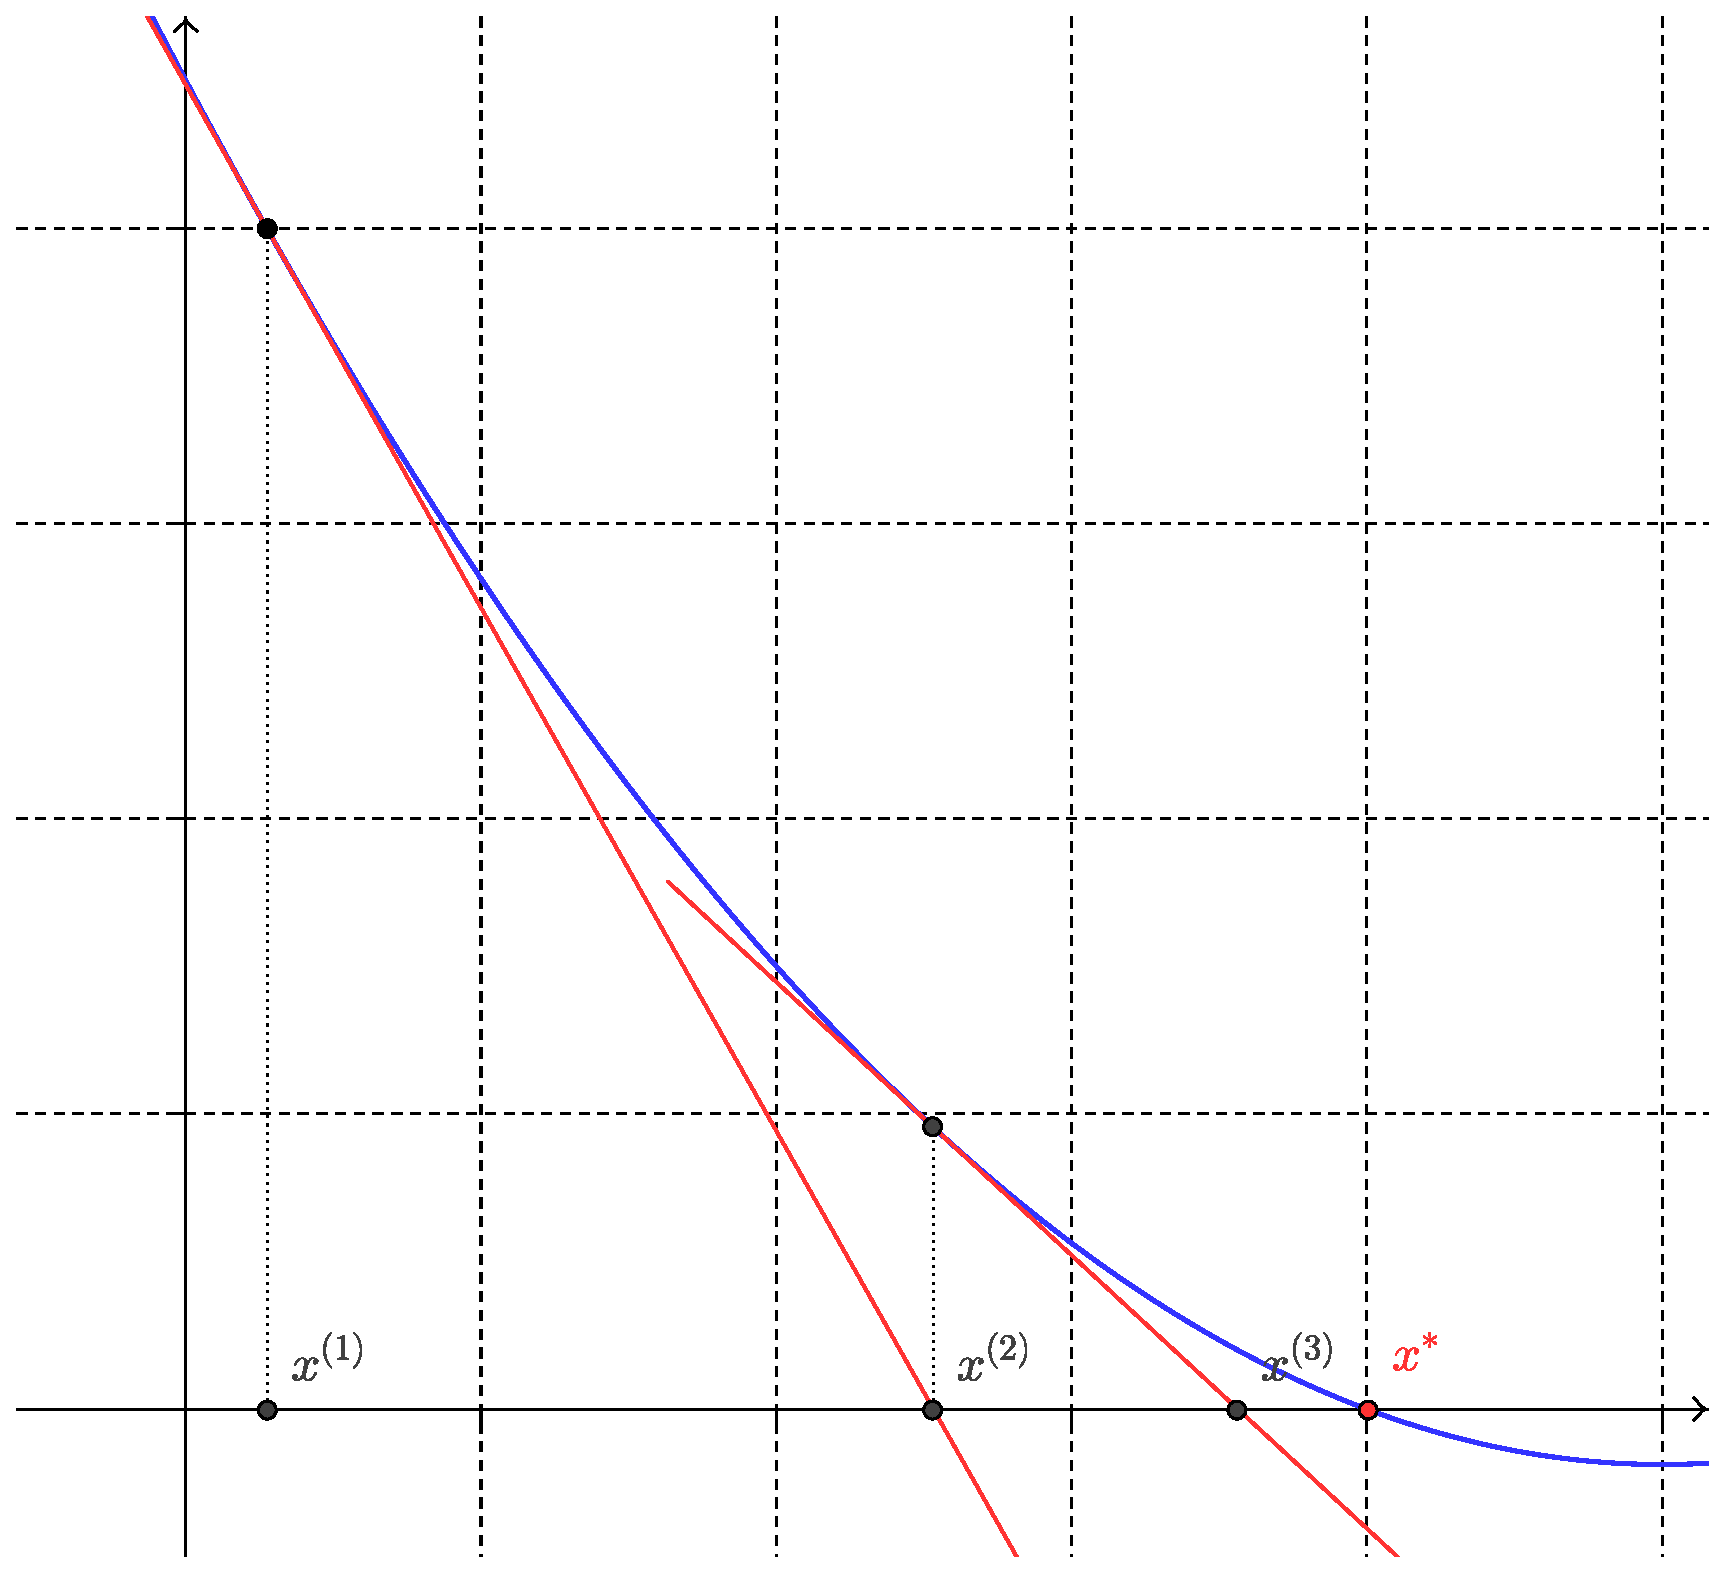
\includegraphics[width=0.8\textwidth]{./cap_eq1d/dados/fig_Newton_geointerp/fig_Newton_geointerp}
  \caption{Interpretação geométrica das iterações de Newton. Veja no \href{https://github.com/phkonzen/notas/blob/master/src/MatematicaNumerica/cap_eq1d/dados/fig_Newton_geointerp/fig_Newton_geointerp.ggb}{Geogebra}.}
  \label{fig:Newton_geointerp}
\end{figure}


Destas observações, concluímos que a iterada $x^{(k+1)}$ do método de Newton corresponde ao ponto de interseção da reta tangente ao gráfico da $f$ pelo ponto $(x^{k}, f(x^{k}))$. Veja a Figura \ref{fig:Newton_geointerp}.

\begin{ex}\label{ex:Newton_init}
  Consideremos que o método de Newton seja usado para aproximarmos o zero de
  \begin{equation}
    f(x) = (x-1)e^{-x^2}.
  \end{equation}
Observemos que esta função tem $x=1$ como seu único zero. Agora, se escolhermos $x^{(1)} = 0,5$ as iterações de Newton convergem para este zero, mas, se escolhermos $x^{(1)}=1,5$ não (veja a Tabela \ref{tab:ex_Newton_init}).

\begin{table}[h!]
  \centering
  \begin{tabular}{r|cc}
    $k$ & $x^{(k)}$ & $x^{(k+1)}$ \\\hline
    1 & $5,0000\E-1$ & $1,5000\E+0$ \\
    2 & $8,3333\E-1$ & $2,5000\E+0$ \\
    3 & $9,6377\E-1$ & $2,7308\E+0$ \\
    4 & $9,9763\E-1$ & $2,9355\E+0$ \\
    5 & $9,9999\E-1$ & $3,1223\E+0$ \\
    6 & $1,0000\E+0$ & $3,2955\E+0$ \\
    7 & $1,0000\E+0$ & $3,4580\E+0$ \\\hline    
  \end{tabular}
  \caption{Resultados referentes ao Exemplo \ref{ex:Newton_init}}
  \label{tab:ex_Newton_init}
\end{table}

  \begin{figure}[h!]
    \centering
    \includegraphics[width=0.8\textwidth]{./cap_eq1d/dados/ex_Newton_init/fig_ex_Newton_init}
    \caption{Escolha da aproximação inicial para o método de Newton.}
    \label{fig:ex_Newton_init}
  \end{figure}

Embora ambas aproximações iniciais estão a mesma distância da solução $x=1$, quando tomamos $x^{(1)}=1,5$ as iterações irão divergir, como podemos observar da interpretação geométrica dada na Figura \ref{fig:ex_Newton_init}.
\end{ex}

\subsection{Análise de convergência}

Seja $x^*$ o zero de uma dada função $f$ duas vezes continuamente diferenciável com $f'(x)\neq 0$ para todo $x\in [x^*-\varepsilon_0, x^*+\varepsilon_0]$ para algum $\varepsilon_0>0$. Seja, também, $(x^{(k)})_{k=1}^\infty$ a sequência das iteradas de Newton
\begin{equation}\label{eq:newton_iter1}
  x^{(k+1)} = x^{(k)} - \frac{f(x^{(k)})}{f'(x^{(k)})},\quad k=1, 2, \ldots,
\end{equation}
com aproximação inicial $x^{(1)}\in (x^*-\varepsilon_0, x^*+\varepsilon_0)$. Então, do polinômio de Taylor de grau 1 de $f$ em torno de $x^{(1)}$, temos
\begin{equation}
  f(x^*) = f(x^{(1)}) + f'(x^{(1)})(x^* - x^{(1)}) + \frac{f''(\xi^{(1)})}{2!}(x^*-x^{(1)})^2,
\end{equation}
onde $\xi^{(1)}$ está entre $x^{(1)}$ e $\xi$. Daí, rearranjamos os termos e notamos que $f(x^*)=0$ para obtermos
\begin{equation}
  x^* - \left[x^{(1)} - \frac{f(x^{(1)})}{f'(x^{(1)})}\right] = \frac{f''(\xi^{(1)})}{2f'(x^{(1)})}(x^*-x^{(1)})^2.
\end{equation}
Então, da iteração de Newton \eqref{eq:newton_iter1}, temos
\begin{equation}
  x^* - x^{(2)} = \frac{f''(\xi^{(1)})}{2f'(x^{(1)})}(x^* - x^{(1)})^2
\end{equation}
Logo,
\begin{equation}\label{eq:newton_taxa_1}
  |x^* - x^{(2)}| \leq C |x^* - x^{(1)}|^2,
\end{equation}
com
\begin{equation}
  C = \sup_{x,y\in [x^*-\varepsilon, x^*+\varepsilon]} \left|\frac{f''(x)}{2f'(y)}\right|.
\end{equation}
Segue, então, que se $x^{(1)}\in (x^*-\varepsilon, x^* + \varepsilon)$ para algum $\varepsilon>0$ tal que
\begin{equation}
  C |x^* - x|^2 < 1,\quad\forall x\in (x^*-\varepsilon, x^* + \varepsilon),
\end{equation}
então $x^{(2)}\in (x^*-\varepsilon, x^*+\varepsilon)$.

Logo, por indução matemática\footnote{Veja o exercício \ref{ex:Newton_analise_conv}.}, temos que o método de Newton tem taxa de convergência quadrática
\begin{equation}\label{eq:Newton_taxa_quadratica}
  |x^{(k+1)}-x^*| \leq C|x^{(k)}-x^{*}|^{\pmb{2}},
\end{equation}
para qualquer escolha de $x^{(1)}$ suficientemente próximo de $x^*$, i.e. $x^{(1)}\in (x^*-\varepsilon, x^*+\varepsilon)$.

\begin{obs}
  O intervalo $(x^*-\varepsilon, x^*+\varepsilon)$ é chamado de \emph{bacia de atração}\index{bacia de atração} do método de Newton.
\end{obs}

\begin{ex}\label{ex:Newton_taxa}
  Retornamos ao problema de encontrar o zero da função
  \begin{equation}
    f(x) = \sen^2\left(x+\frac{\pi}{4}\right) - x^3 + \frac{\pi}{4}x^2 + \frac{5\pi^2}{16}x + \frac{3\pi^3}{64}.
  \end{equation}
  no intervalo $[2,3]$. Este problema foi construído de forma que $x^* = 3\pi/4$ é um zero de $f$. Então, fazendo as iterações de Newton com aproximação inicial $x^{(1)}=2,6$, obtemos os resultados apresentados na Tabela \ref{tab:ex_Newton_taxa}, os quais evidenciam a convergência quadrática das iterações computadas.

\begin{table}[h!]
  \centering
  \begin{tabular}{r|cc}
    $k$ & $x^{(k)}$ & $|x^{(k)}-x^*|$ \\\hline
    1 & $2,6000$ & $2,4\E-01$ \\
    2 & $2,3836$ & $2,7\E-02$ \\
    3 & $2,3566$ & $3,9\E-04$ \\
    4 & $2,3562$ & $8,3\E-08$ \\
    5 & $2,3562$ & $3,6\E-15$ \\\hline
  \end{tabular}
  \caption{Resultados referentes ao Exemplo \ref{ex:Newton_taxa}.}
  \label{tab:ex_Newton_taxa}
\end{table}

\ifisoctave
Os resultados apresentados na Tabela \ref{tab:ex_Newton_taxa} podem ser computados no \verb+GNU Octave+ com o seguinte \href{https://github.com/phkonzen/notas/blob/master/src/MatematicaNumerica/cap_eq1d/dados/ex_Newton_taxa/ex_Newton_taxa.m}{código}:
\verbatiminput{./cap_eq1d/dados/ex_Newton_taxa/ex_Newton_taxa.m}
\fi
\end{ex}

\subsection{Zeros de multiplicidade par}

Na análise de convergência acima foi necessário assumir que $f'(x) \neq 0$ para todo $x$ em uma vizinha do zero $x^*$ da função $f$. Isto não é possível no caso de $x^*$ ser um zero de multiplicidade par pois, neste caso, $f'(x^*) = 0$. Neste caso, podemos aplicar o método de Newton a $f'(x)$, a qual tem $x^*$ como um zero de multiplicidade ímpar.

\begin{ex}\label{ex:Newton_multpar}
  Consideremos o problema de aproximar o zero da função
  \begin{equation}
    f(x) = \sen^2\left(x+\frac{\pi}{4}\right) - x^3 + \frac{\pi}{4}x^2 + \frac{5\pi^2}{16}x + \frac{3\pi^3}{64}.
  \end{equation}
  no intervalo $[-1,0]$. Este problema foi construído de forma que $x^* = -\pi/4$ é um zero de multiplicidade par de $f$. Então, aplicamos o método de Newton a
  \begin{equation}
    f'(x) = 2\sen\left(x+\frac{\pi}{4}\right)\cos\left(x+\frac{\pi}{4}\right) -3x² +\frac{\pi}{2}x+\frac{5\pi^2}{16}.
  \end{equation}
Ou seja, as iterações de Newton são
\begin{equation}
  x^{(k+1)} = x^{(k)} - \frac{f'(x^{(k)})}{f''(x^{(k)})},\quad k=1,2,\ldots,
\end{equation}
sendo $x^{(1)}$ uma aproximação inicial. Na Tabela~\ref{tab:ex_Newton_multpar}, temos os resultados obtidos da computação destas iterações com $x^{(1)}=-0,5$.

\begin{table}[h!]
  \centering
  \begin{tabular}{r|cc}
    $k$ & $x^{(k)}$ & $|x^{(k)}-x^*|$ \\\hline
    1 & $-5,0000\E-1$ & $2,9\E-01$ \\
    2 & $-8,3407\E-1$ & $4,9\E-02$ \\
    3 & $-7,8619\E-1$ & $7,9\E-04$ \\
    4 & $-7,8540\E-1$ & $2,3\E-07$ \\
    5 & $-7,8540\E-1$ & $1,9\E-14$ \\\hline
  \end{tabular}
  \caption{Resultados referentes ao Exemplo \ref{ex:Newton_multpar}.}
  \label{tab:ex_Newton_multpar}
\end{table}

\ifisoctave
Os resultados apresentados na Tabela \ref{tab:ex_Newton_multpar} podem ser computados no \verb+GNU Octave+ com o seguinte \href{https://github.com/phkonzen/notas/blob/master/src/MatematicaNumerica/cap_eq1d/dados/ex_Newton_multpar/ex_Newton_multpar.m}{código}:
\verbatiminput{./cap_eq1d/dados/ex_Newton_multpar/ex_Newton_multpar.m}
\fi
\end{ex}

\subsection*{Exercícios}

\begin{exer}\label{exer:Newton_1}
  Use o método de Newton para obter uma aproximação do zero de $f(x)=x^3\sen(x)-\cos(x)$ no intervalo $[0,5, 1]$ com precisão de $10^{-6}$.
\end{exer}
\begin{resp}
    \ifisoctave 
  \href{https://github.com/phkonzen/notas/blob/master/src/MatematicaNumerica/cap_eq1d/dados/exer_Newton_1/exer_Newton_1.m}{Código.} 
  \fi
  $9,15811\times 10^{-1}$
\end{resp}

\begin{exer}\label{exer:Newton_multpar}
  Use o método de Newton para obter uma aproximação do zero de
  \begin{equation}
    f(x) = (-x^2+1,154x-0,332929)\cos(x) + x^2 - 1,154x + 0,332929
  \end{equation}
no intervalo $(0,55, ~0,65)$ com precisão de $10^-5$.
\end{exer}
\begin{resp}
    \ifisoctave 
  \href{https://github.com/phkonzen/notas/blob/master/src/MatematicaNumerica/cap_eq1d/dados/exer_Newton_multpar/exer_Newton_multpar.m}{Código.} 
  \fi
  $5,7700\times 10^{-1}$
\end{resp}

\begin{exer}\label{ex:Newton_analise_conv}
  Complete a demonstração por indução matemática de que o método de Newton tem taxa de convergência quadrática.
\end{exer}

\section{Método da secante}\label{cap_eq1d_sec_secante}

O método da secante é uma variação do método de Newton. Observemos que para duas aproximações $x^{(k)}$ e $x^{(k-1)}$ suficientemente próximas, temos\footnote{Razão fundamental do Cálculo.}
\begin{equation}
  f'(x^{(k)}) \approx \frac{f(x^{(k)})-f(x^{(k-1)})}{x^{(k)}-x^{(k-1)}}.
\end{equation}
Assim sendo, substituindo esta aproximação em \eqref{eq:Newton_iteracao}, obtemos as iterações do método da secante:
\begin{align}
  x^{(1)}&, x^{(2)} = \text{aprox. iniciais},\\
  x^{(k+1)} &= x^{(k)} - f(x^{(k)})\frac{x^{(k)}-x^{(k-1)}}{f(x^{(k)})-f(x^{(k-1)})},
\end{align}
para $k=2,3,\ldots$.

\begin{ex}\label{ex:secante_exec}
  Consideremos o problema de encontrar o zero da função
  \begin{equation}
    f(x) = \sen^2\left(x+\frac{\pi}{4}\right) - x^3 + \frac{\pi}{4}x^2 + \frac{5\pi^2}{16}x + \frac{3\pi^3}{64}.
  \end{equation}
  no intervalo $[2,3]$. Então, fazendo as iterações do método da secante com aproximações iniciais $x^{(1)}=2,6$ e $x^{(2)}-2,5$, obtemos os resultados apresentados na Tabela \ref{tab:ex_secante_exec}.

\begin{table}[h!]
  \centering
  \begin{tabular}{r|ccc}
    $k$ & $x^{(k-1)}$ & $x^{(k)}$ & $|x^{(k)}-x^{(k-1)}|$ \\\hline
    2 & $2,6000$ & $2,5000$ & -x-\\
    3 & $2,5000$ & $2.3728$ & $1,3\E-1$ \\
    4 & $2,3728$ & $2,3574$ & $1,5\E-2$ \\
    5 & $2,3574$ & $2,3562$ & $1,2\E-3$ \\
    6 & $2,3562$ & $2,3562$ & $1,1\E-5$ \\
    7 & $2,3562$ & $2,3562$ & $7,0\E-9$ \\\hline
  \end{tabular}
  \caption{Resultados referentes ao Exemplo \ref{ex:secante_exec}.}
  \label{tab:ex_secante_exec}
\end{table}

\ifisoctave
Os resultados apresentados na Tabela \ref{tab:ex_secante_exec} podem ser computados no \verb+GNU Octave+ com o seguinte \href{https://github.com/phkonzen/notas/blob/master/src/MatematicaNumerica/cap_eq1d/dados/ex_secante_exec/ex_secante_exec.m}{código}:
\verbatiminput{./cap_eq1d/dados/ex_secante_exec/ex_secante_exec.m}
\fi
\end{ex}

\subsection{Interpretação geométrica}

A iteração do método da secante é
\begin{equation}
  x^{(k+1)} = x^{(k)} - f(x^{(k)})\frac{x^{(k)}-x^{(k-1)}}{f(x^{(k)})-f(x^{(k-1)})},
\end{equation}
donde segue que
\begin{equation}
  0 = x^{(k+1)}-x^{(k)} + f(x^{(k)})\frac{x^{(k)}-x^{(k-1)}}{f(x^{(k)})-f(x^{(k-1)})},
\end{equation}
bem como que
\begin{equation}\label{eq:secante_geointerp}
  0 = \frac{f(x^{(k)})-f(x^{(k-1)})}{x^{(k)}-x^{(k-1)}}(x^{(k+1)}-x^{(k)}) + f(x^{(k)}).
\end{equation}
Agora, observemos que
\begin{equation}
  y = \frac{f(x^{(k)})-f(x^{(k-1)})}{x-x^{(k-1)}}(x^{(k+1)}-x^{(k)}) + f(x^{(k)}).
\end{equation}
é a equação da reta secante ao gráfico de $f$ pelos pontos $(x^{(k)}, f(x^{(k)}))$ e $(x^{(k-1)}, f(x^{(k-1)}))$. 

Do observado acima, temos que \eqref{eq:secante_geointerp} nos mostra que a iterada $x^{(k+1)}$ é a a interseção do eixo $x$ com a reta secante ao gráfico de $f$ pelos pontos $(x^{(k)}, f(x^{(k)}))$ e $(x^{(k-1)}, f(x^{(k-1)}))$. Veja a Figura \ref{fig:secante_geointerp}.


\begin{figure}[h!]
  \centering
  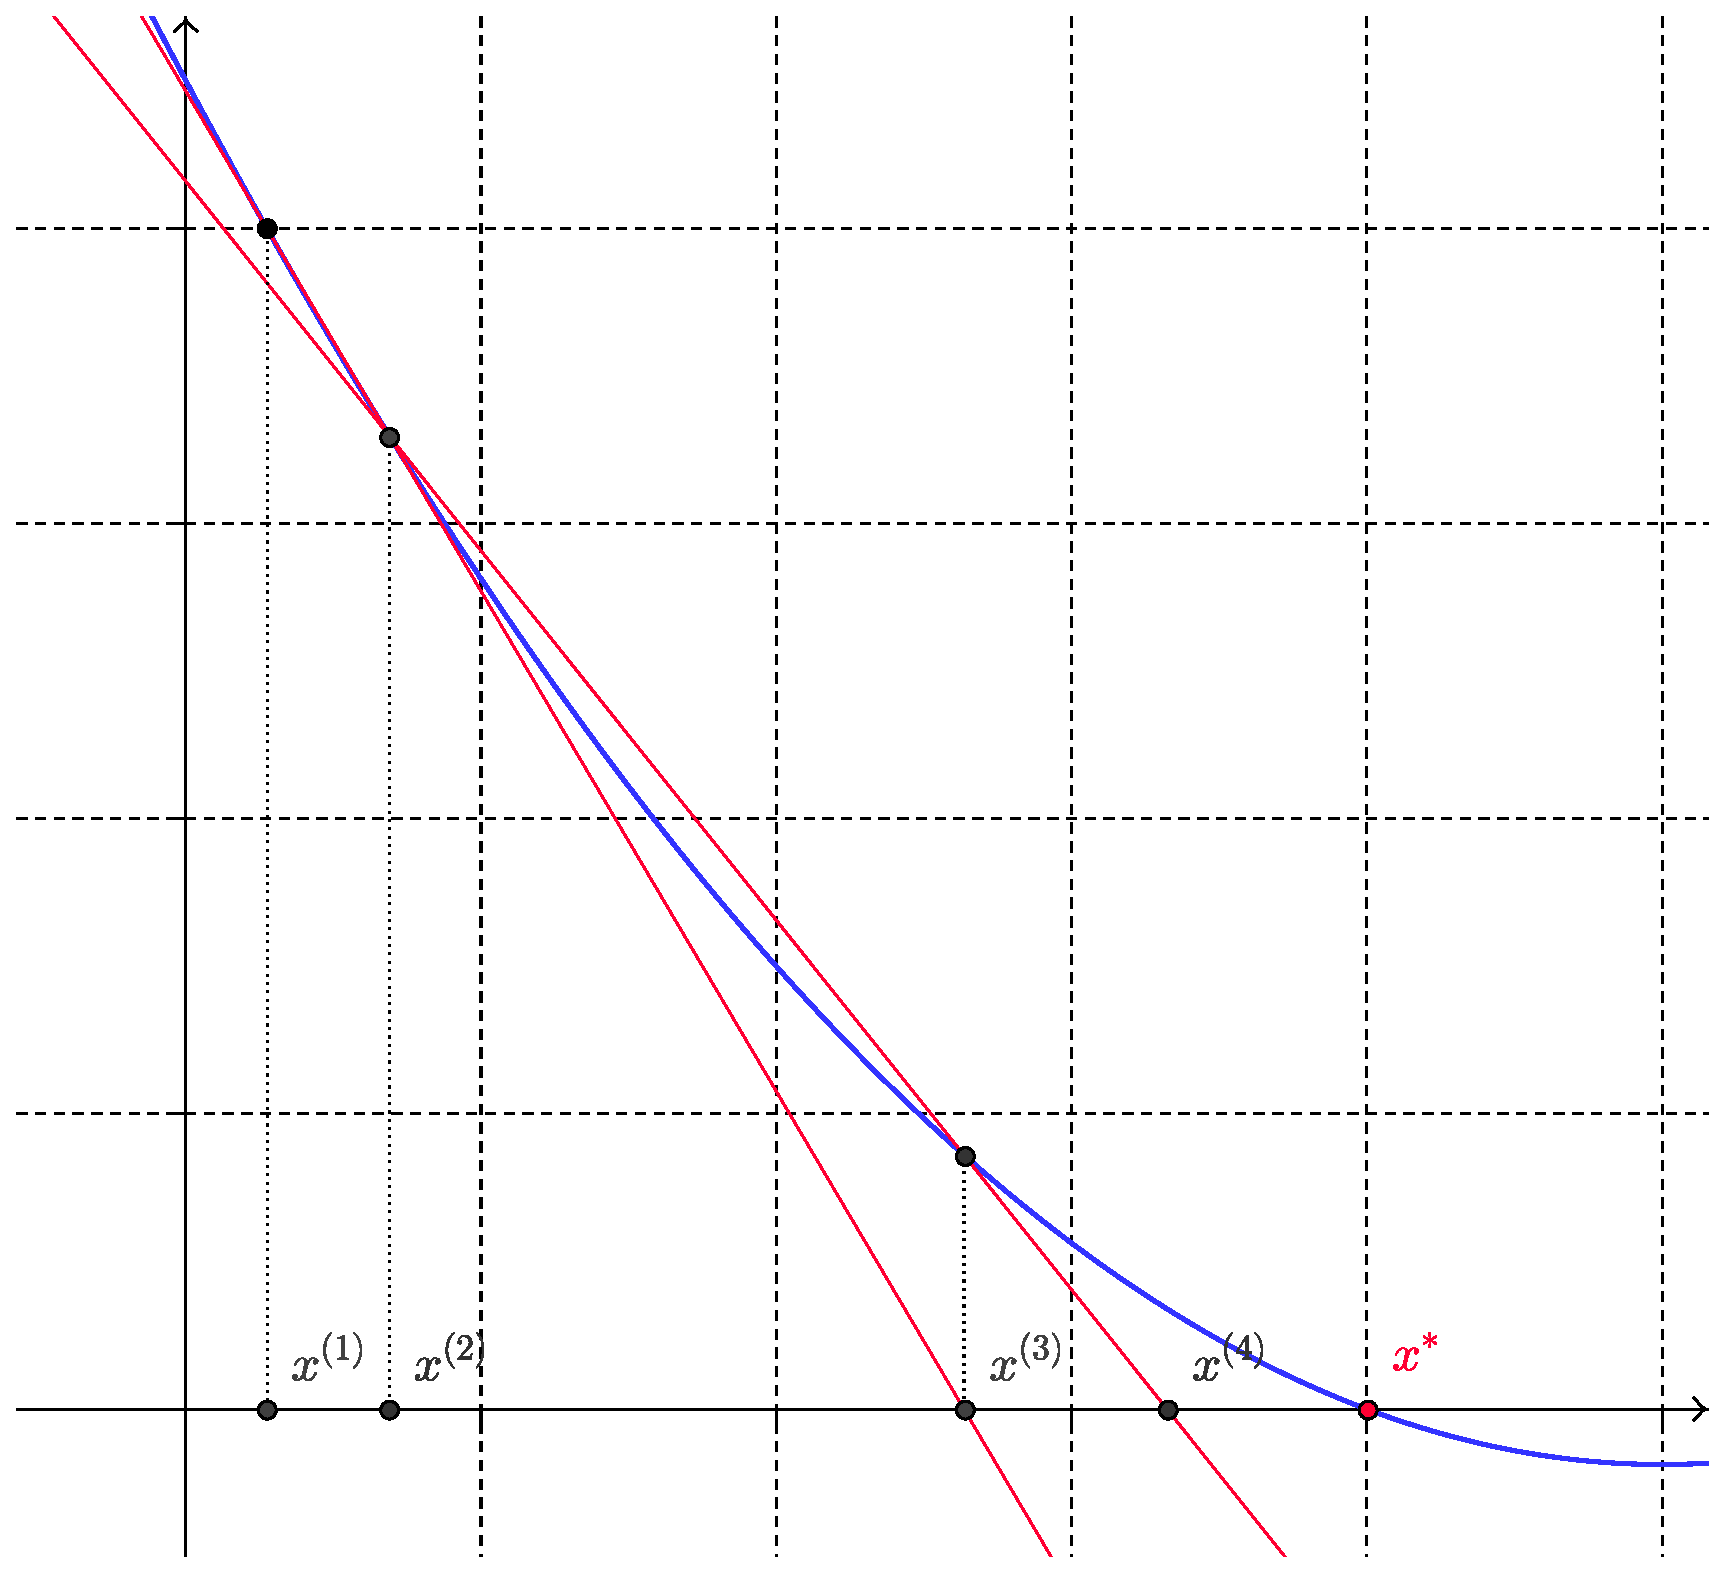
\includegraphics[width=0.8\textwidth]{./cap_eq1d/dados/fig_secante_geointerp/fig_secante_geointerp}
  \caption{Interpretação geométrica das iterações do método da secante. Veja no \href{https://github.com/phkonzen/notas/blob/master/src/MatematicaNumerica/cap_eq1d/dados/fig_secante_geointerp/fig_secante_geointerp.ggb}{Geogebra}.}
  \label{fig:secante_geointerp}
\end{figure}


\begin{obs}
  A interpretação geométrica do método da secante pode nos ajudar a escolher as aproximações iniciais $x^{(1)}$ e $x^{(2)}$. Como uma boa prática, escolhemo-las próximas do zero (por inspeção gráfica), tomando $x^{(2)}$ como uma aproximação melhor que $x^{(1)}$. 
\end{obs}

\subsection{Análise de convergência}

Pode-se mostrar\footnote{Veja, por exemplo, \href{https://www.ufrgs.br/reamat/CalculoNumerico/livro-oct/sdeduv-metodo_das_secantes.html}{Seção 3.5.2 do livro ``Cálculo Numérico''} do projeto \href{https://www.ufrgs.br/reamat}{REAMAT}.} que a taxa de convergência do método da secante é superlinear com
\begin{equation}
  |x^{(k+1)}-x^*| \leq C|x^{(k)}-x^*|^{\pmb{\varphi}},
\end{equation}
onde $\varphi = (1+\sqrt{5})/2\approx 1,618$ (razão áurea) e $x^*$ é o zero de $f$.


\begin{ex}\label{ex:secante_taxa}
  Consideremos o problema de encontrar o zero da função
  \begin{equation}
    f(x) = \sen^2\left(x+\frac{\pi}{4}\right) - x^3 + \frac{\pi}{4}x^2 + \frac{5\pi^2}{16}x + \frac{3\pi^3}{64}.
  \end{equation}
  no intervalo $[2,3]$. Este problema foi construído de forma que $x^* = 3\pi/4$ é um zero de $f$. Agora, fazendo as iterações do método da secante com aproximações iniciais $x^{(1)}=2,6$ e $x^{(2)}=2,5$, obtemos os resultados apresentados na Tabela \ref{tab:ex_secante_taxa}.

\begin{table}[h!]
  \centering
  \begin{tabular}{r|cc}
    $k$ & $x^{(k)}$ & $|x^{(k)}-x^*|$ \\\hline
    3 & $2,3728$ & $1,7\E-02$ \\
    4 & $2,3574$ & $1,2\E-03$ \\
    5 & $2,3562$ & $1,1\E-05$ \\
    6 & $2,3562$ & $7,0\E-09$ \\\hline
  \end{tabular}
  \caption{Resultados referentes ao Exemplo \ref{ex:secante_taxa}.}
  \label{tab:ex_secante_taxa}
\end{table}

\ifisoctave
Os resultados apresentados na Tabela \ref{tab:ex_secante_taxa} podem ser computados no \verb+GNU Octave+ com o seguinte \href{https://github.com/phkonzen/notas/blob/master/src/MatematicaNumerica/cap_eq1d/dados/ex_secante_taxa/ex_secante_taxa.m}{código}:
\verbatiminput{./cap_eq1d/dados/ex_secante_taxa/ex_secante_taxa.m}
\fi
\end{ex}


\begin{obs}(\normalfont{Zeros de multiplicidade par.})
  A taxa de convergência superlinear do método da secante não se mantém para o caso de $x^*$ ser um zero de multiplicidade par. Para contornar isso, pode-se aplicar o método à derivada da $f$.
\end{obs}

\begin{obs}(\normalfont{Cancelamento catastrófico.})
  Conforme convergem as iterações do método da secante, o denominador $f(x^{(k)})-f(x^{(k-1)})$ pode convergir rapidamente para zero, ocasionando uma divisão por zero.
\end{obs}


\subsection*{Exercícios}

\begin{exer}\label{exer:secante_1}
  Use o método da secante para obter uma aproximação do zero de $f(x)=x^3\sen(x)-\cos(x)$ no intervalo $[0,5, 1]$ com precisão de $10^{-5}$.
\end{exer}
\begin{resp}
    \ifisoctave 
  \href{https://github.com/phkonzen/notas/blob/master/src/MatematicaNumerica/cap_eq1d/dados/exer_secante_1/exer_secante_1.m}{Código.} 
  \fi
  $9,1581\times 10^{-1}$
\end{resp}

\begin{exer}\label{exer:secante_multpar}
  Use o método da secante para obter uma aproximação do zero de
  \begin{equation}
    f(x) = (-x^2+1,154x-0,332929)\cos(x) + x^2 - 1,154x + 0,332929
  \end{equation}
no intervalo $(0,55, ~0,65)$ com precisão de $10^-5$.
\end{exer}
\begin{resp}
    \ifisoctave 
  \href{https://github.com/phkonzen/notas/blob/master/src/MatematicaNumerica/cap_eq1d/dados/exer_secante_multpar/exer_secante_multpar.m}{Código.} 
  \fi
  $5,7700\times 10^{-1}$
\end{resp}

%Este trabalho está licenciado sob a Licença Atribuição-CompartilhaIgual 4.0 Internacional Creative Commons. Para visualizar uma cópia desta licença, visite http://creativecommons.org/licenses/by-sa/4.0/deed.pt_BR ou mande uma carta para Creative Commons, PO Box 1866, Mountain View, CA 94042, USA.

\chapter{Sistemas Lineares}\label{cap_sislin}
\thispagestyle{fancy}

\begin{flushright}
  [Vídeo] | [Áudio] | \href{https://phkonzen.github.io/notas/contato.html}{[Contatar]}
\end{flushright}

Neste capítulo, apresentam-se métodos numéricos para a resolução de sistemas lineares de grande porte.

\section{Teste}\label{cap_teste}

\begin{flushright}
  [Vídeo] | [Áudio] | \href{https://phkonzen.github.io/notas/contato.html}{[Contatar]}
\end{flushright}


% %Este trabalho está licenciado sob a Licença Atribuição-CompartilhaIgual 4.0 Internacional Creative Commons. Para visualizar uma cópia desta licença, visite http://creativecommons.org/licenses/by-sa/4.0/deed.pt_BR ou mande uma carta para Creative Commons, PO Box 1866, Mountain View, CA 94042, USA.

\chapter{Métodos iterativos para sistemas lineares}\label{cap_sl_iter}
\thispagestyle{fancy}

\section{Métodos de Jacobi e de Gauss-Seidel}\label{cap_sl_iter_sec_jgs}

Nesta seção, discutiremos os métodos de Jacobi\footnote{Carl Gustav Jacob Jacobi, 1804 - 1851, matemático alemão. Fonte: \href{https://en.wikipedia.org/wiki/Carl_Gustav_Jacob_Jacobi}{Wikipedia}.} e de Gauss-Seidel\footnote{Johann Carl Friedrich Gauss, 1777 - 1855, matemático alemão. Philipp Ludwig von Seidel, 1821 - 1896, matemático alemão. Fonte: \href{https://en.wikipedia.org/wiki/Philipp_Ludwig_von_Seidel}{Wikipedia}.} para a aproximação da solução de sistemas lineares.

\subsection{Método de Jacobi}

Dado um sistema $A\pmb{x} = \pmb{b}$ com $n$ equações e $n$ incógnitas, consideramos a seguinte decomposição da matriz $A = L + D + U$:
\begin{align}
  A &=
  \begin{bmatrix}
    a_{11} & a_{12} & a_{13} & \ldots & a_{1n}\\
    a_{21} & a_{22} & a_{23} & \ldots & a_{2n}\\
    a_{31} & a_{32} & a_{33} & \ldots & a_{3n}\\
    \vdots & \vdots & \vdots & \ldots & \vdots\\
    a_{n1} & a_{n2} & a_{n3} & \ldots & a_{nn}\\
  \end{bmatrix}\\
    &= \underbrace{\begin{bmatrix}
    0 & 0 & 0 & \ldots & 0\\
    a_{21} & 0 & 0 & \ldots & 0\\
    a_{31} & a_{32} & 0 & \ldots & 0\\
    \vdots & \vdots & \vdots & \ldots & \vdots\\
    a_{n1} & a_{n2} & a_{n3} & \ldots & 0\\
  \end{bmatrix}}_{L}\\
    &+ \underbrace{\begin{bmatrix}
    a_{11} & 0 & 0 & \ldots & 0\\
    0 & a_{22} & 0 & \ldots & 0\\
    0 & 0 & a_{33} & \ldots & 0\\
    \vdots & \vdots & \vdots & \ldots & \vdots\\
    0 & 0 & 0 & \ldots & a_{nn}\\
  \end{bmatrix}}_{D}\\
  &+ \underbrace{\begin{bmatrix}
    0 & a_{12} & a_{13} & \ldots & a_{1n}\\
    0 & 0 & a_{23} & \ldots & a_{2n}\\
    0 & 0 & a_{33} & \ldots & a_{3n}\\
    \vdots & \vdots & \vdots & \ldots & \vdots\\
    0 & 0 & 0 & \ldots & a_{nn}\\
  \end{bmatrix}}_{U}.
\end{align}
Isto é, a matriz $A$ decomposta como a soma de sua parte triangular inferior $L$, de sua diagonal $D$ e de sua parte triangular superior $U$.

Desta forma, podemos reescrever o sistema $A\pmb{x}=b$ da seguinte forma:
\begin{align}
  A\pmb{x} = \pmb{b} &\Leftrightarrow (L + D + U)\pmb{x} = \pmb{b}\\
         &\Leftrightarrow D\pmb{x} = -(L+U)\pmb{x} + \pmb{b}\\
         &\Leftrightarrow \pmb{x} = -D^{-1}(L+U)\pmb{x} + D^{-1}\pmb{b}.
\end{align}
Ou seja, resolver o sistema $A\pmb{x} = \pmb{b}$ é equivalente a resolver o problema de ponto fixo
\begin{equation}
  \pmb{x} = T_J\pmb{x} + \pmb{c}_J,
\end{equation}
onde $T_J = -D^{-1}(L+U)$ é chamada de \emph{matriz de Jacobi}\index{matriz de!Jacobi} e $\pmb{c}_J = D^{-1}\pmb{b}$ é chamado de \emph{vetor de Jacobi}\index{vetor de!Jacobi}.

\begin{ex}\label{ex:jacobi_intro}
  Consideremos o sistema linear $A\pmb{x} = \pmb{b}$ com
  \begin{equation}
    A =
    \begin{bmatrix}
      -4 & 2 & -1 \\
      -2 & 5 & 2 \\
       1 & -1 & -3
    \end{bmatrix},\quad
    \pmb{b} =
    \begin{bmatrix}
      -11\\ -7\\ 0
    \end{bmatrix}.
  \end{equation}
  Este sistema tem solução $\pmb{x} = (2, -1, 1)$. Neste caso, temos a decomposição $A = L + D + U$ com
  \begin{equation}
    L = \begin{bmatrix} 
      0 & 0 & 0 \\
      -2 & 0 & 0 \\
       1 & -1 & 0
     \end{bmatrix},\quad
    D = \begin{bmatrix}
      -4 & 0 & 0 \\
      0 & 5 & 0 \\
       0 & 0 & -3                  
     \end{bmatrix}
  \end{equation}
  e
  \begin{equation}
    U = \begin{bmatrix}
      0 & 2 & -1 \\
      0 & 0 & 2 \\
       0 & 0 & 0
    \end{bmatrix}.
  \end{equation}
  Ainda, observamos que
  \begin{align}
    T_J\pmb{x} + \pmb{c}_J &= -D^{-1}(L+U)\pmb{x} + D^{-1}\pmb{b}\\
    &= \underbrace{\begin{bmatrix}
        0 & 1/2 & 1/4 \\
        2/5 & 0 & -2/5 \\
        1/3 & -1/3 & 0
      \end{bmatrix}}_{T_J}
      \underbrace{\begin{bmatrix}
        2 \\
        -1 \\
        1             
      \end{bmatrix}}_{\pmb{x}} +
      \underbrace{\begin{bmatrix}
       11/4 \\
       -7/5 \\
       0
      \end{bmatrix}}_{\pmb{c}_J}\\
  &= \underbrace{\begin{bmatrix}
        2 \\
        -1 \\
        1             
      \end{bmatrix}}_{\pmb{x}}.
  \end{align}
\ifisoctave
No \verb+GNU Octave+, podemos fazer as computações acima com o seguinte \href{https://github.com/phkonzen/notas/blob/master/src/MatematicaNumerica/cap_sl_iter/dados/ex_jacobi_intro/ex_jacobi_intro.m}{código}:
\verbatiminput{./cap_sl_iter/dados/ex_jacobi_intro/ex_jacobi_intro.m}
\fi
\end{ex}

Com o exposto acima, o \emph{método de Jacobi} consiste na seguinte iteração de ponto fixo
\begin{align}
  \pmb{x}^{(1)} &= \text{aprox. inicial},\\
  \pmb{x}^{(k+1)} &= T_J\pmb{x}^{(k)} + \pmb{c}_J,\label{eq:iter_jacobi_mat}
\end{align}
onde $\pmb{x}^{(k)} = (x_1^{(k)}, x_2^{(k)}, \dotsc, x_n^{(k)})$ é a $k$-ésima aproximação (ou iterada) de Jacobi.

A iteração \eqref{eq:iter_jacobi_mat} pode ser equivalentemente escrita na seguinte forma algébrica
\begin{equation}
  x_i^{(k+1)} = \frac{{\displaystyle b_i - \sum_{\overset{j=1}{j\neq i}}^n a_{ij}x^{(k)}}}{a_{ii}},~i=1, 2, \dotsc, n,
\end{equation}
a qual não requer a computação da matriz $T_J$ e $\pmb{c}_J$.

\begin{ex}\label{ex:jacobi_exec}
  Consideremos o sistema $A\pmb{x} = \pmb{b}$ com
  \begin{equation}
    A =
    \begin{bmatrix}
      -4 & 2 & -1 \\
      -2 & 5 & 2 \\
       1 & -1 & -3
    \end{bmatrix},\quad
    \pmb{b} =
    \begin{bmatrix}
      -11\\ -7\\ 0
    \end{bmatrix}.
  \end{equation}
  Aplicando o método de Jacobi com aproximação inicial $\pmb{x}^{(1)} = (0, 0, 0)$ obtemos os resultados da Tabela \ref{tab:ex_jacobi_exec}.

  \begin{table}[h!]
    \centering
    \begin{tabular}{l|cc}
      k & $\pmb{x}^{(k)}$ & $\|A\pmb{x}^{(k)}-\pmb{b}\|$\\\hline
      1 & $(0,0,~0,0,~0,0)$ & $1,3\E+1$\\
      2 & $(2,8,~-1,4,~0,0)$ & $7,4\E+0$ \\
      3 & $(2,0,~-0,3,~1,4)$ & $4,6\E+0$ \\
      4 & $(2,3,~-1,1,~0,8)$ & $2,2\E+0$ \\
      5 & $(2,0,~-0,8,~1,1)$ & $1,4\E+0$ \\
      6 & $(2,1,~-1,1,~0,9)$ & $6,9\E-1$ \\
      7 & $(2,0,~-0,9,~1,0)$ & $4,2\E-1$ \\
      8 & $(2,0,~-1,0,~1,0)$ & $2,2\E-1$ \\
      9 & $(2,0,~-1,0,~1,0)$ & $1,3\E-1$ \\
      10 & $(2,0,~-1,0,~1,0)$ & $6,9\E-2$ \\\hline
    \end{tabular}
    \caption{Resultados referentes ao Exemplo \ref{ex:jacobi_exec}.}
    \label{tab:ex_jacobi_exec}
  \end{table}

\ifisoctave
No \verb+GNU Octave+, podemos obter os resultados reportados na Tabela \ref{tab:ex_jacobi_exec} com o seguinte \href{https://github.com/phkonzen/notas/blob/master/src/MatematicaNumerica/cap_sl_iter/dados/ex_jacobi_exec/ex_jacobi_exec.m}{código}:
\verbatiminput{./cap_sl_iter/dados/ex_jacobi_exec/ex_jacobi_exec.m}
\fi
\end{ex}

\subsection{Método de Gauss-Seidel}

Como acima, começamos considerando um sistema linear $A\pmb{x} = \pmb{b}$ e a decomposição $A = L + D + U$, onde $L$ é a parte triangular inferior de $A$, $D$ é sua parte diagonal e $U$ sua parte triangular superior. Então, observamos que
\begin{align}
  A\pmb{x} = \pmb{b} &\Leftrightarrow (L + D + U)\pmb{x} = \pmb{b}\\
  &\Leftrightarrow (L+D)\pmb{x} = -U\pmb{x} + \pmb{b}\\
  &\Leftrightarrow \pmb{x} = -(L+D)^{-1}U\pmb{x} + (L+D)^{-1}\pmb{b}.
\end{align}
Isto nos leva a iteração de Gauss-Seidel
\begin{align}
  \pmb{x}^{(1)} = \text{aprox. inicial},\\
  \pmb{x}^{(k+1)} = T_G\pmb{x}^{(k)} + \pmb{c}_G,\label{eq:iter_gs_mat}
\end{align}
onde $T_G = -(L+D)^{-1}U$ é a chamada \emph{matriz de Gauss-Seidel}\index{matriz de!Gauss-Seidel} e $\pmb{c}_G = (L+D)^{-1}\pmb{b}$ é o chamado \emph{vetor de Gauss-Seidel}\index{vetor de!Gauss-Seidel}.

Observamos, também, que a iteração \eqref{eq:iter_gs_mat} pode ser reescrita na seguinte forma algébrica
\begin{equation}
  x_i^{(k+1)} = \frac{{\displaystyle b_i - \sum_{j=1}^{i-1} a_{ij}x^{(k+1)} - \sum_{j=i+1}^{n} a_{ij}x^{(k)}}}{a_{ii}},~i=1, 2, \dotsc, n.
\end{equation}

\begin{ex}\label{ex:gs_exec}
  Consideremos o sistema $A\pmb{x} = \pmb{b}$ com
  \begin{equation}
    A =
    \begin{bmatrix}
      -4 & 2 & -1 \\
      -2 & 5 & 2 \\
       1 & -1 & -3
    \end{bmatrix},\quad
    \pmb{b} =
    \begin{bmatrix}
      -11\\ -7\\ 0
    \end{bmatrix}.
  \end{equation}
  Aplicando o método de Gauss-Seidel com aproximação inicial $\pmb{x}^{(1)} = (0, 0, 0)$ obtemos os resultados da Tabela \ref{tab:ex_gs_exec}.

  \begin{table}[h!]
    \centering
    \begin{tabular}{l|cc}
      k & $\pmb{x}^{(k)}$ & $\|A\pmb{x}^{(k)}-\pmb{b}\|$\\\hline
      1 & $(0,0,~0,0,~0,0)$ & $1,3\E+1$ \\
      2 & $(2,8,~-0,3,~1,0)$ & $2,6\E+0$ \\
      3 & $(2,3,~-0,9,~1,1)$ & $1,2\E+0$ \\
      4 & $(2,0,~-1,0,~1,0)$ & $2,5\E-1$ \\
      5 & $(2,0,~-1,0,~1,0)$ & $4,0\E-2$ \\\hline
    \end{tabular}
    \caption{Resultados referentes ao Exemplo \ref{ex:gs_exec}.}
    \label{tab:ex_gs_exec}
  \end{table}

\ifisoctave
No \verb+GNU Octave+, podemos obter os resultados reportados na Tabela \ref{tab:ex_gs_exec} com o seguinte \href{https://github.com/phkonzen/notas/blob/master/src/MatematicaNumerica/cap_sl_iter/dados/ex_gs_exec/ex_gs_exec.m}{código}:
\verbatiminput{./cap_sl_iter/dados/ex_gs_exec/ex_gs_exec.m}
\fi
\end{ex}

\subsection{Análise de convergência}

Observamos que ambos os métodos de Jacobi e de Gauss-Seidel consistem de iterações da forma
\begin{equation}
  \pmb{x}^{(k+1)} = T\pmb{x}^{(k)} + \pmb{c},~k=1, 2, \ldots,\label{eq:jgs_iter}
\end{equation}
com $x^{(1)}$ uma aproximação inicial dada, $T$ e $c$ a matriz e o vetor de iteração, respectivamente. O seguinte teorema nos fornece uma condição suficiente e necessária para a convergência de tais métodos.

\begin{teo}
  Para qualquer $\pmb{x}^{(1)}\in\mathbb{R}^n$, temos que a sequência $\{\pmb{x}^{(k+1)}\}_{k=1}^{\infty}$ dada por
  \begin{equation}
    \pmb{x}^{(k+1)} = T\pmb{x}^{(k)} + \pmb{c},
  \end{equation}
  converge para a solução única de $\pmb{x} = T\pmb{x} + \pmb{c}$ se, e somente se, $\rho(T) < 1$\footnote{$\rho(T)$ é o raio espectral da matriz $T$, i.e. o máximo dos módulos dos autovalores de $T$.}.
\end{teo}
\begin{dem}
  Veja \cite[Cap. 7, Sec. 7.3]{Burden2015a}.
\end{dem}

\begin{obs}(\normalfont{Taxa de convergência})
  Para uma iteração da forma \eqref{eq:jgs_iter}, vale
  \begin{equation}
    \|\pmb{x}^{(k)}-\pmb{x}\| \approx \rho(T)^{k-1}\|\pmb{x}^{(1)}-\pmb{x}\|,
  \end{equation}
onde $\pmb{x}$ é a solução de $\pmb{x} = T\pmb{x} + \pmb{c}$.
\end{obs}

\begin{ex}\label{ex:jacobi_exec}
  Consideremos o sistema $A\pmb{x} = \pmb{b}$ com
  \begin{equation}
    A =
    \begin{bmatrix}
      -4 & 2 & -1 \\
      -2 & 5 & 2 \\
       1 & -1 & -3
    \end{bmatrix},\quad
    \pmb{b} =
    \begin{bmatrix}
      -11\\ -7\\ 0
    \end{bmatrix}.
  \end{equation}
  Nos Exemplos \ref{ex:jacobi_exec} e \ref{ex:gs_exec} vimos que ambos os métodos de Jacobi e de Gauss-Seidel eram convergentes, sendo que este convergiu aproximadamente duas vezes mais rápido que esse. Isto é confirmado pelos raios espectrais das respectivas matrizes de iteração
  \begin{equation}
    \rho(T_J) \approx 0,56,\quad\rho(T_G) \approx 0,26.
  \end{equation}

\ifisoctave
No \verb+GNU Octave+, podemos obter os raios espectrais das matrizes de iteração de Jacobi e Gauss-Seidel com o seguinte \href{https://github.com/phkonzen/notas/blob/master/src/MatematicaNumerica/cap_sl_iter/dados/ex_jgs_conv/ex_jgs_conv.m}{código}:
\verbatiminput{./cap_sl_iter/dados/ex_jgs_conv/ex_jgs_conv.m}
\fi
\end{ex}

\begin{obs}{\normalfont{Matriz estritamente diagonal dominante}}
  Pode-se mostrar que se $A$ é uma matriz estritamente diagonal dominante, i.e. se
  \begin{equation}
    |a_{ii}| > \sum_{\overset{j=1}{j\neq i}}^n |a_{ij}|,~\forall i=1, 2, \ldots, n,
  \end{equation}
então ambos os métodos de Jacobi e de Gauss-Seidel são convergentes.
\end{obs}

\subsection*{Exercícios}

\begin{exer}\label{exer:jacobi_exec}
  Considere o seguinte sistema linear
  \begin{align}
    -4x_1 + x_2 + x_3 - x_4 &= -1\\
    5x_2 -x_3 + 2x_4 &= 3\\
    -x_1 + 4x_3 - 2x_4 &= -2\\
    x_1 -x_2 -5x_4 &= 1
  \end{align}
  Compute a quinta iterada $x^{(5)}$ do método de Jacobi aplicado a este sistema com aproximação inicial $x^{(1)} = (1, 1, -1, -1)$. Também, compute $\|Ax^{(5)} - b\|$.
\end{exer}
\begin{resp}
    \ifisoctave 
    \href{https://github.com/phkonzen/notas/blob/master/src/MatematicaNumerica/cap_sl_iter/dados/exer_jacobi_exec/exer_jacobi_exec.m}{Código.} 
  \fi
  $x^{(5)} = (-1,00256,~2,95365,~-1,95347,~0,97913)$; $\|Ax^{(5)}-b\| = 0,42244$
\end{resp}

\begin{exer}\label{exer:gs_exec}
  Considere o seguinte sistema linear
  \begin{align}
    -4x_1 + x_2 + x_3 - x_4 &= -1\\
    5x_2 -x_3 + 2x_4 &= 3\\
    -x_1 + 4x_3 - 2x_4 &= -2\\
    x_1 -x_2 -5x_4 &= 1
  \end{align}
  Compute a quinta iterada $x^{(5)}$ do método de Gauss-Seidel aplicado a este sistema com aproximação inicial $x^{(1)} = (1, 1, -1, -1)$. Também, compute $\|Ax^{(5)} - b\|$.
\end{exer}
\begin{resp}
    \ifisoctave 
    \href{https://github.com/phkonzen/notas/blob/master/src/MatematicaNumerica/cap_sl_iter/dados/exer_gs_exec/exer_gs_exec.m}{Código.} 
  \fi
  $x^{(5)} = (-1,00423,~3,00316,~-2,00401,~0,99852)$; $\|Ax^{(5)}-b\| = 0,025883$
\end{resp}

\section{Método do gradiente}\label{cap_sl_iter_sec_metg}

Começamos observando que se $A$ é uma matriz $n\times n$ positiva definida\footnote{$A$ é simétrica e $x^TAx > 0$ para todo $x\neq 0$.}, temos que $\pmb{x}\in\mathbb{R}^n$ é solução de
\begin{equation}\label{eq:metg_sislin}
  A\pmb{x} = \pmb{b}
\end{equation}
se, e somente se, $\pmb{x}$ é solução do seguinte problema de minimização
\begin{equation}\label{eq:metg_minprob}
  \min_{\pmb{x}\in\mathbb{R}^n}f(\pmb{x}) := \frac{1}{2}\pmb{x}^TA\pmb{x}-\pmb{x}^T\pmb{b}.
\end{equation}

O método do gradiente é um algoritmo da forma: dada uma aproximação inicial $\pmb{x}^{(1)}$ da solução de \eqref{eq:metg_minprob} (ou, equivalentemente, de \eqref{eq:metg_sislin}), computamos novas aproximações da forma iterativa
\begin{equation}
  \pmb{x}^{(k+1)} = \pmb{x}^{(k)} + \alpha^{(k)}\pmb{d}^{(k)},\quad k=1, 2, \ldots,
\end{equation}
onde $\alpha^{(k)}$ é o tamanho do passo (um escalar) e $\pmb{d}^{(k)}\in\mathbb{R}^n$ é a direção de busca.

Para escolhermos a direção $\pmb{d}^{(k)}$, tomamos a fórmula de Taylor de $f$ em torno da aproximação $\pmb{x}^{(k)}$
\begin{equation}\label{eq:metg_taylor}
  f(\pmb{x}^{(k+1)}) = f(\pmb{x}^{(k)}) + \alpha^{(k)}\nabla f(\pmb{x}^{(k)})\cdot \pmb{d}^{(k)} + O\left((\alpha^{(k)})^2\right),
\end{equation}
com $\alpha^{(k)}\to 0$, onde $\nabla f$ denota o gradiente de $f$, i.e.
\begin{align}
  \nabla f(\pmb{x}^{(k)}) &= \left(\frac{\p f}{\p x_1}(\pmb{x}^{(k)}), \frac{\p f}{\p x_2}(\pmb{x}^{(k)}), \dotsc, \frac{\p f}{\p x_n}(\pmb{x}^{(k)})\right)\\
  &= A\pmb{x}^{(k)}-\pmb{b}.
\end{align}


De \eqref{eq:metg_taylor}, segue que se
\begin{equation}
  \nabla f(\pmb{x}^{(k)})\cdot \pmb{d}^{(k)} < 0,
\end{equation}
então $f(\pmb{x}^{(k+1)}) < f(\pmb{x}^{(k)})$ se $\alpha^{(k)}$ é suficientemente pequeno. Em particular, podemos escolher
\begin{equation}
  \pmb{d}^{(k)} = -\nabla f(\pmb{x}^{(k)}),
\end{equation}
se $\nabla f(\pmb{x}^{(k)})\neq 0$.

Do exposto acima, temos a \pmb{iteração do método do gradiente}
\begin{align}
  \pmb{x}^{(1)} &= \text{aprox. inicial}\\
  \pmb{x}^{(k+1)} &= \pmb{x}^{(k)} - \alpha^{(k)}\pmb{r}^{(k)},~k=1, 2, \ldots,
\end{align}
onde $\pmb{r}^{(k)}$ é o resíduo da iterada $k$ dado por
\begin{equation}
  \pmb{r}^{(k)} = A\pmb{x^{(k)}}-\pmb{b}.
\end{equation}

\begin{ex}\label{ex:metg_pc}
  Consideremos o sistema $Ax = b$ com
  \begin{equation}
    A =
    \begin{bmatrix}
      2 & -1 & 0 & 0\\
      -1 & 2 & -1 & 0\\
      0 & -1 & 2 & -1 \\
      0 & 0 & -1 & 2
    \end{bmatrix},\quad
    b =
    \begin{bmatrix}
      -3\\
      2\\
      2\\
      -3
    \end{bmatrix}.
  \end{equation}
  Na Tabela \ref{tab:metg_pc} temos os resultados do emprego do método do gradiente com $\pmb{x}^{(1)} = (0, 0, 0, 0)$ e com passo constante $\alpha^{(k)}\equiv 0,5$.

  \begin{table}[h!]
    \centering
    \begin{tabular}{l|c|c}
      k & $\pmb{x}^{(k)}$ & $\|A\pmb{x}^{(k)}-\pmb{b}\|$\\\hline
      1 & $(0,0,~0,0,~0,0,~0,0)$ & $5,1\E+0$\\
      2 & $(-1,5,~1,0,~1,0,~-1,5)$ & $1,6\E+0$\\
      3 & $(-1,0,~0,8,~0,8,~-1,0)$ & $5,0\E-1$\\
      4 & $(-1,1,~0,9,~0,9,~-1,1)$ & $1,8\E-1$\\
      5 & $(-1,1,~0,9,~0,9,~-1,1)$ & $8,8\E-2$\\
      6 & $(-1,1,~0,9,~0,9,~-1,1)$ & $6,2\E-2$\\
      7 & $(-1,0,~0,9,~0,9,~-1,0)$ & $4,9\E-2$\\
      8 & $(-1,0,~0,9,~0,9,~-1,0)$ & $4,0\E-2$\\
      9 & $(-1,0,~0,9,~0,9,~-1,0)$ & $3,2\E-2$\\
      10 & $(-1,0,~1,0,~1,0,~-1,0)$ & $2,6\E-2$\\
      11 & $(-1,0,~1,0,~1,0,~-1,0)$ & $2,1\E-2$\\\hline
    \end{tabular}
    \caption{Resultados referentes ao Exemplo \ref{ex:metg_pc}.}
    \label{tab:metg_pc}
  \end{table}

\ifisoctave
No \verb+GNU Octave+, podemos fazer as computações acima com o seguinte \href{https://github.com/phkonzen/notas/blob/master/src/MatematicaNumerica/cap_sl_iter/dados/ex_metg_pc/ex_metg_pc.m}{código}:
\verbatiminput{./cap_sl_iter/dados/ex_metg_pc/ex_metg_pc.m}
\fi
\end{ex}

\subsection{Escolha do passo}

Da iteração do método do gradiente, temos que a melhor escolha do passo $\alpha^{(k)}$ é tal que
\begin{equation}
  f(\pmb{x}^{(k)}+\alpha^{(k)}\pmb{r}^{(k)}) = \min_{\alpha > 0} f(\pmb{x}^{(k)}+\alpha\pmb{r}^{(k)}).
\end{equation}
Desta forma,
\begin{align}
  \frac{\dd}{\dd \alpha}f(\pmb{x}^{(k)}+\alpha \pmb{r}^{(k)}) = 0 &\Rightarrow \nabla f(\pmb{x}^{(k+1)})\cdot \pmb{r}^{(k)} = 0,\\
  &\Rightarrow \left(A(\pmb{x}^{(k)}+\alpha^{(k)}\pmb{r}^{(k)})-b\right)\cdot\pmb{r}^{(k)} = 0,\\
  &\Rightarrow (A\pmb{x}^{(k)}-\pmb{b})\cdot\pmb{r}^{(k)}+\alpha^{(k)}\pmb{r}^{(k)}\cdot A\pmb{r}^{(k)} = 0,
\end{align}
donde
\begin{equation}
  \alpha^{(k)} = - \frac{\pmb{r}^{(k)}\cdot\pmb{r}^{(k)}}{\pmb{r}^{(k)}\cdot A\pmb{r}^{(k)}}.
\end{equation}

\begin{ex}\label{ex:metg_alpha}
  Consideremos o sistema $Ax = b$ com
  \begin{equation}
    A =
    \begin{bmatrix}
      2 & -1 & 0 & 0\\
      -1 & 2 & -1 & 0\\
      0 & -1 & 2 & -1 \\
      0 & 0 & -1 & 2
    \end{bmatrix},\quad
    b =
    \begin{bmatrix}
      -3\\
      2\\
      2\\
      -3
    \end{bmatrix}.
  \end{equation}
  Na Tabela \ref{tab:metg_alpha} temos os resultados do emprego do método do gradiente com $\pmb{x}^{(1)} = (0, 0, 0, 0)$ e com passo
  \begin{equation}
    \alpha^{(k)} = - \frac{\pmb{r}^{(k)}\cdot\pmb{r}^{(k)}}{\pmb{r}^{(k)}\cdot A\pmb{r}^{(k)}}.
\end{equation}

  \begin{table}[h!]
    \centering
    \begin{tabular}{l|c|c}
      k & $\pmb{x}^{(k)}$ & $\|A\pmb{x}^{(k)}-\pmb{b}\|$\\\hline
      1 & $(0,0,~0,0,~0,0,~0,0)$ & $5,1\E+0$\\
      2 & $(-1,1,~0,8,~0,8,~-1,1)$ & $1,5\E-1$\\
      3 & $(-1,0,~1,0,~1,0,~-1,0)$ & $3,0\E-2$\\
      4 & $(-1,0,~1,0,~1,0,~-1,0)$ & $8,8\E-4$\\
      5 & $(-1,0,~1,0,~1,0,~-1,0)$ & $1,8\E-4$\\\hline
    \end{tabular}
    \caption{Resultados referentes ao Exemplo \ref{ex:metg_alpha}.}
    \label{tab:metg_alpha}
  \end{table}

\ifisoctave
No \verb+GNU Octave+, podemos fazer as computações acima com o seguinte \href{https://github.com/phkonzen/notas/blob/master/src/MatematicaNumerica/cap_sl_iter/dados/ex_metg_alpha/ex_metg_alpha.m}{código}:
\verbatiminput{./cap_sl_iter/dados/ex_metg_alpha/ex_metg_alpha.m}
\fi
\end{ex}

\subsection*{Exercícios}

\emconstrucao

\section{Método do gradiente conjugado}\label{cap_sl_iter_sec_metgc}

O método do gradiente conjugado é uma variação do método do gradiente (veja Seção \ref{cap_sl_iter_sec_metg}). Aqui, a solução de um dado sistema $A\pmb{x}=\pmb{b}$, com $A$ uma matriz positiva definida, é computada de forma iterativa por
\begin{align}
  \pmb{x}^{(1)} &= \text{aprox. inicial},\\
  \pmb{d}^{(1)} &= \pmb{r}^{(1)},\\
  &\\
  \pmb{x}^{(k+1)} &= \pmb{x}^{(k)} + \alpha_k\pmb{d}^{(k)},\\
  \alpha^{(k)} &= -\frac{\pmb{r}^{(k)}\cdot \pmb{d}^{(k)}}{\pmb{d}^{(k)}\cdot A\pmb{d}^{(k)}},\\
  \pmb{d}^{(k+1)} &= -\pmb{r}^{(k+1)}+\beta_k\pmb{d}^{(k)},\\
  \beta^{(k)} &= \frac{\pmb{r}^{(k+1)}\cdot A\pmb{d}^{(k)}}{\pmb{d}^{(k)}\cdot A\pmb{d}^{(k)}},
\end{align}
para $k = 1, 2, \ldots$, e $\pmb{r}^{(k)} = A\pmb{x}^{(k)}-\pmb{b}$.

\begin{ex}\label{ex:metgc_exec}
  Consideremos o sistema $Ax = b$ com
  \begin{equation}
    A =
    \begin{bmatrix}
      2 & -1 & 0 & 0\\
      -1 & 2 & -1 & 0\\
      0 & -1 & 2 & -1 \\
      0 & 0 & -1 & 2
    \end{bmatrix},\quad
    b =
    \begin{bmatrix}
      -3\\
      2\\
      2\\
      -3
    \end{bmatrix}.
  \end{equation}
  Na Tabela \ref{tab:metgc_exec} temos os resultados do emprego do método do gradiente conjugado com $\pmb{x}^{(1)} = (0, 0, 0, 0)$.

  \begin{table}[h!]
    \centering
    \begin{tabular}{l|c|c}
      k & $\pmb{x}^{(k)}$ & $\|A\pmb{x}^{(k)}-\pmb{b}\|$\\\hline
      1 & $(0,~0,~0,~0)$ & $5.1\E+0$\\
      2 & $(-1,1,~0,8,~0,8,~-1,1)$ & $1,5\E-1$\\
      3 & $(-1,0,~1,0,~1,0,~-1,0)$ & $0,0\E+0$\\\hline
    \end{tabular}
    \caption{Resultados referentes ao Exemplo \ref{ex:metgc_exec}.}
    \label{tab:metg_alpha}
  \end{table}

\ifisoctave
No \verb+GNU Octave+, podemos fazer as computações acima com o seguinte \href{https://github.com/phkonzen/notas/blob/master/src/MatematicaNumerica/cap_sl_iter/dados/ex_metgc_exec/ex_metgc_exec.m}{código}:
\verbatiminput{./cap_sl_iter/dados/ex_metgc_exec/ex_metgc_exec.m}
\fi
\end{ex}

\subsection*{Exercícios}

\emconstrucao


\chapter{Métodos para Sistemas Não Lineares}\label{cap_snl}

Neste capítulo, estudamos sobre \hl{métodos para a resolução} de sistemas de equações não lineares. Vamos tratar o caso \hl{de problemas da forma}: encontrar $\pmb{x}\in\mathbb{R}^n$ tal que
\begin{equation}\hleq
  F(\pmb{x}) = \pmb{0},
\end{equation}
onde $F:\mathbb{R}^n\to\mathbb{R}^n$ é uma dada função vetorial.

\section{Método de Newton}\label{cap_snl_sec_newton}

Consideramos o problema de encontrar
\begin{equation}
  \pmb{x} = (x_1, x_2, \dotsc, x_n)\in\mathbb{R}^n
\end{equation}
tal que
\begin{equation}\label{cap_snl_sec_newton:eq:prob0}\hleq
  F(\pmb{x}) = \pmb{0},
\end{equation}
onde $F:\mathbb{R}^n\to\mathbb{R}^n$ é uma dada função vetorial com
\begin{equation}
  F(\pmb{x}) = (f_1(\pmb{x}), f_2(\pmb{x}), \dotsc, f_n(\pmb{x}))\in\mathbb{R}^n.
\end{equation}

Sejam \hl{$\pmb{x}^*$ a solução exata} de \eqref{cap_snl_sec_newton:eq:prob0} e \hl{$\pmb{x}^{(0)}$ uma dada aproximação de $\pmb{x}^*$}. Assim sendo, tomamos a seguinte \hl{expansão de $F$ em polinômio de Taylor}{\taylor}:
\begin{equation}\hleq
  F(\pmb{x}^*) = F(\pmb{x}^{(0)}) + J_F(\pmb{x}^{(0)})(\pmb{x}^*-\pmb{x}^{(0)}) + \pmb{r},
\end{equation}
onde $J_F$ é a \hl{\emph{matriz jacobiana}{\jacobi} de $F$}
\begin{align}
  \hleq{J_F(\pmb{x})} &:= \frac{\p(f_1, f_2, \dotsc, f_n)}{\p(x_1, x_2, \dotsc, x_n)}\\
  &\hleq{:= \begin{bmatrix}
    \frac{\p f_1}{\p x_1} & \frac{\p f_1}{\p x_2} & \ldots & \frac{\p f_1}{\p x_n}\\
    \frac{\p f_2}{\p x_1} & \frac{\p f_2}{\p x_2} & \ldots & \frac{\p f_2}{\p x_n}\\
    \vdots & \vdots & \vdots & \vdots \\
    \frac{\p f_n}{\p x_1} & \frac{\p f_n}{\p x_2} & \ldots & \frac{\p f_n}{\p x_n}\\
  \end{bmatrix}}
\end{align}
e $\|\pmb{r}\|^2\to 0$ quando $\|\pmb{x}^{(0)}-\pmb{x}^*\|\to 0$. 

Daí, como $F(\pmb{x}^*) = \pmb{0}$, segue que
\begin{equation}
  J_F(\pmb{x}^{(0)})(\pmb{x}^*-\pmb{x}^{(0)}) \approx -F(\pmb{x}^{(0)}).
\end{equation}
Então, multiplicando a inversa da jacobiana à esquerda, obtemos
\begin{equation}
  \pmb{x}^*-\pmb{x}^{(0)} \approx - J_F^{-1}(\pmb{x}^{(0)})F(\pmb{x}^{(0)})
\end{equation}
e, também,
\begin{equation}
  \pmb{x}^* \approx \pmb{x}^{(0)} - J_F^{-1}(\pmb{x}^{(0)})F(\pmb{x}^{(0)}).
\end{equation}

O exposto acima nos motiva a \hl{\emph{iteração de Newton}}{\newton}:
\begin{subequations}\hleq
  \begin{align}
    &\pmb{x}^{(0)} = \text{aprox. inicial},\\
    &\pmb{x}^{(k+1)} = \pmb{x}^{(k)} - J_F^{-1}(\pmb{x}^{(k)})F(\pmb{x}^{(k)}),
  \end{align}
\end{subequations}
com $k=0, 1, 2, \ldots$.

\begin{ex}\label{cap_snl_sec_newton:ex:newton_intro}
  Seja o sistema de equações não lineares
  \begin{subequations}
    \begin{align}
      & x_1x_2^2 = x_1^2x_2 - 6,\\
      & x_1^2x_2^3 - 7 = -x_1.
    \end{align}
  \end{subequations}
  Para usarmos o método de Newton, reescrevemos o sistema na seguinte forma
  \begin{subequations}
    \begin{align}
      x_1x_2^2 - x_1^2x_2 + 6 &= 0,\\
      x_1 + x_1^2x_2^3 - 7 &= 0.
    \end{align}
\end{subequations}
  Com isso, identificamos a função objetivo
  \begin{align}
    F(\pmb{x}) &=
    \begin{bmatrix}
      f_1(\pmb{x})\\
      f_2(\pmb{x})
    \end{bmatrix}\\
    &=
    \begin{bmatrix}
      x_1x_2^2 - x_1^2x_2 + 6\\
      x_1 + x_1^2x_2^3 - 7
    \end{bmatrix}
  \end{align}
  e calculamos sua matriz jacobiana
  \begin{align}
    J_F(\pmb{x}) &= \frac{\p(f_1, f_2)}{\p(x_1, x_2)} \\
                 &=
                   \begin{bmatrix}
                     \frac{\p f_1}{\p x_1} & \frac{\p f_1}{\p x_2}\\
                     \frac{\p f_2}{\p x_1} & \frac{\p f_2}{\p x_2}\\
                   \end{bmatrix}\\
                 &=
                   \begin{bmatrix}
                     x_2^2 - 2x_1x_2 & 2x_1x_2-x_1^2\\
                     1+2x_1x_2^3 & 3x_1^2x_2^2
                   \end{bmatrix}
  \end{align}
  Definidas $F$ e $J_F$ e tomando a aproximação inicial
  \begin{equation}
    \pmb{x}^{(0)} = (-1.5, 1.5)
  \end{equation}
  computamos as iterações de Newton e obtemos os resultados apresentados na Tabela \ref{cap_snl_sec_newton:tab:newton_intro}.

  \begin{table}[H]
    \centering
    \caption{Resultados referentes ao Exemplo \ref{cap_snl_sec_newton:ex:newton_intro}.}
    \begin{tabular}{lcc}\toprule
      k & $\pmb{x}^{(k)}$ & $\|F(\pmb{x}^{(k)})\|$\\\midrule
      0 & $(-1.50, 1.50)$ & $1.2\E+0$\\
      1 & $(-1.07, 1.82)$ & $1.2\E+0$\\
      2 & $(-9.95\E-1, 2.00)$ & $7.6\E-2$\\
      3 & $(-1.00, 2.00)$ & $1.2\E-4$ \\
      4 & $(-1.00, 2.00)$ & $2.1\E-9$ \\\bottomrule
    \end{tabular}
    \label{cap_snl_sec_newton:tab:newton_intro}
  \end{table}

\begin{lstlisting}
import numpy as np
import numpy.linalg as npla

def newton(F, J, x0, 
           maxiter=100, tol=1.49e-8):
  print(f'\n{0}: x = {x0}, ' + \
        f'norm = {npla.norm(F(x0)):.1e}')
  info = -1
  for k in range(maxiter):
    x = x0 - npla.inv(J(x0))@F(x0)
    print(f'{k+1}: x = {x}, ' + \
          f'norm = {npla.norm(F(x)):.1e}')
    if (npla.norm(x - x0) < tol):
      info = 0
      break
    x0 = x.copy()
  return x, info

def F(x):
  n = x.size
  y = np.empty(n)
  y[0] = x[0]*x[1]**2 - x[0]**2*x[1] + 6
  y[1] = x[0] + x[0]**2*x[1]**3 - 7
  return y

def J(x):
  n = x.size
  y = np.empty((n,n))
  y[0,0] = x[1]**2 - 2*x[0]*x[1]
  y[0,1] = 2*x[0]*x[1] - x[0]**2
  y[1,0] = 1 + 2*x[0]*x[1]**3
  y[1,1] = 3*x[0]**2*x[1]**2
  return y

x0 = np.array([-1.5, 1.5])
x, info = newton(F, J, x0)
\end{lstlisting}

\end{ex}

\subsection{Análise Numérica}

Para uma função $F$ suficientemente suave e com uma escolha apropriada da aproximação inicial $\pmb{x}^{(0)}$, temos que as \hl{iterações de Newton}
\begin{equation}
  \pmb{x}^{(k+1)} = \pmb{x}^{(k)} - J_F^{-1}(\pmb{x}^{(k)})F(\pmb{x}^{(k)}),
\end{equation}
com $k=0, 1, 2, \ldots$, \hl{são quadraticamente convergentes}\endnote{Para informações mais precisas sobre a convergência do Método de Newton, consulte \cite[Seção 5.3]{Stoer1993a}.}, i.e.
\begin{equation}\hleq
  \|\pmb{x}^{(k+1)} - \pmb{x}^*\| \leq C\|\pmb{x}^{(k)}-\pmb{x}^*\|^2,
\end{equation}
onde $\pmb{x}^*$ é a solução exata, i.e. $F(\pmb{x}^*) = \pmb{0}$.

\begin{ex}\label{cap_snl_sec_newton:ex:newton_conv}
  Consideremos o seguinte sistema de equações não lineares
  \begin{align}
    x_1x_2^2 - x_1^2x_2 + 6 &= 0,\\
    x_1 + x_1^2x_2^3 - 7 &= 0.
  \end{align}
  A Figura \ref{cap_snl_sec_newton:fig:ex_newton_conv} é um esboço do gráfico da $\|F(\cdot)\|$. Este problema foi confeccionado de forma que $\pmb{x}^* = (-1, 2)$. Então, tomando $\pmb{x}^{(0)} = (1.5, 1.5)$ como aproximação inicial, computamos as iterações de Newton para este problema, donde obtemos os resultados reportados na Tabela \ref{cap_snl_sec_newton:tab:ex_newton_conv}. 

  \begin{figure}[h!]
    \centering
    \includegraphics[width=0.7\textwidth]{./cap_snl/dados/ex_newton_conv/ex_newton_conv}
    \caption{Esboço do gráfico de $\|F(\cdot)\|$ referente ao Exemplo \ref{cap_snl_sec_newton:ex:newton_conv}.}
    \label{cap_snl_sec_newton:fig:ex_newton_conv}
  \end{figure}

  \begin{table}[H]
    \centering
    \begin{tabular}{lcc}
      k & $\pmb{x}^{(k)}$ & $\|\pmb{x}^{(k)} - \pmb{x}^*\|$\\\hline
      0 & $(-1.50, 1.50)$ & $7.1\E-01$\\
      1 & $(-1.07, 1.82)$ & $2.0\E-01$\\
      2 & $(-9.95\E-1, 2.00)$ & $5.1\E-03$\\
      3 & $(-1.00, 2.00)$ & $2.6\E-05$ \\
      4 & $(-1.00, 2.00)$ & $2.0\E-10$ \\
      5 & $(-1.00, 2.00)$ & $3.1\E-16$ \\\hline
    \end{tabular}
    \caption{Resultados referentes ao Exemplo \ref{cap_snl_sec_newton:ex:newton_conv}.}
    \label{cap_snl_sec_newton:tab:ex_newton_conv}
  \end{table}
\end{ex}

\subsection{Exercícios}

\begin{exer}
  Use o Método de Newton para computar uma solução aproximada para o sistema de equações
  \begin{subequations}
    \begin{align}
      & \frac{x_1^2}{3} + x_2^2 = 1\\
      & x_1^2 + \frac{x_2^2}{4} = 1
    \end{align}
  \end{subequations}
\end{exer}
\begin{resp}
  Soluções exatas: $\pmb{x} = \pm\left(\sqrt{\frac{9}{11}}, \sqrt{\frac{8}{11}}\right)$.
\end{resp}

\begin{exer}
  Use o Método de Newton, com aproximação inicial $\pmb{x}^{(0)} = (1.5, 0.5)$ para computar uma solução aproximada para o sistema de equações
  \begin{subequations}
    \begin{align}
      & x_1^2 = \cos(x_1x_2) + 1\\
      & \sen(x_2) = 2\cos(x_1)
    \end{align}
  \end{subequations}
\end{exer}
\begin{resp}
  $\pmb{x} = (1.3468109, 0.4603195)$
\end{resp}

\begin{exer}
  Use o Método de Newton, com aproximação inicial $\pmb{x}^{(0)} = (1, -1)$ para computar uma solução aproximada para o sistema de equações
  \begin{subequations}
    \begin{align}
      & 3x_1 = \cos(x_1x_2) + \frac{1}{2}\\
      & 4x_1^2 + 2x_2x_1 = 0
    \end{align}
  \end{subequations}  
\end{exer}
\begin{resp}
  $\pmb{x} = (4.668417\E-1, -9.368334\E-1)$
\end{resp}

\begin{exer}
  Use o método de Newton para obter uma aproximação de uma solução de
  \begin{align}
    x_2\sen(x_3)+x_1-2&=0,\\
    x_1x_2-\sen(x_2)+0.2&=0,\\
    x_3^2+\cos(x_1x_2)-4.5&=0.
  \end{align}
Para tanto, use $\pmb{x}^{(1)} = (1, -1, -1)$.
\end{exer}
\begin{resp}
  $\pmb{x} = (1.7519\E+0, -2.6202\E-1, -1.8983\E+0)$
\end{resp}

\begin{exer}
  Considere o problema de encontrar os pontos de interseção no plano $x-y$ da elipse
  \begin{equation}
    \frac{x^2}{4} + \frac{y^2}{9} = 1
  \end{equation}
  com a curva
  \begin{equation}
    x = y^2\sqrt{x}.
  \end{equation}
  Escreva o problema na forma $F(\pmb{x}) = \pmb{0}$ e use o Método de Newton para encontrar o ponto de interseção próximo de $(x, y) = (1.5, 1.5)$.
\end{exer}
\begin{resp}
  $x = 1.842996\E+0$, $y = 1.165148\E+0$
\end{resp}

\ifisbook
\subsubsection{Respostas}
\shipoutAnswer
\fi

%%% SECTION %%%

\section{Métodos \textit{Quasi}-Newton}\label{cap_snl_sec_quasi_newton}
\badgeRevisar

\subsection{Método do Acorde}
\badgeRevisar

O método do acorde consiste na seguinte iteração
\begin{align}
  \pmb{x}^{(1)} &= \text{aprox. inicial},\\
  \pmb{x}^{(k+1)} &= \pmb{x}^{(k)} - J_F^{-1}(\pmb{x}^{(1)})F(\pmb{x}^{(k)}).
\end{align}
Ou seja, é a iteração de Newton com jacobina constante.

\begin{ex}\label{ex:acorde_exec}
  Consideremos o seguinte sistema de equações não lineares
  \begin{align}
    x_1x_2^2 - x_1^2x_2 + 6 &= 0,\\
    x_1 + x_1^2x_2^3 - 7 &= 0.
  \end{align}
  Definidas $F$ e $J_F$ e tomando $\pmb{x}^{(1)} = (1.5, 1.5)$ como aproximação inicial, computamos as iterações do método do acorde de forma a obtermos os resultados apresentados na Tabela \ref{tab:ex_acorde_exec}.

  \begin{table}[h!]
    \centering
    \begin{tabular}{lcc}
      k & $\pmb{x}^{(k)}$ & $\|\pmb{x}^{(k)} - \pmb{x}^*\|$\\\hline
      1 & $(-1.50, 1.50)$ & -x- \\
      2 & $(-1.07, 1.82)$ & $5.3\E-1$ \\
      3 & $(-1.02, 1.93)$ & $1.2\E-1$ \\
      4 & $(-1.00, 1.98)$ & $5.2\E-2$ \\
      5 & $(-9.98\E-1, 2.00)$ & $1.8\E-2$ \\
      6 & $(-9.98\E-1, 2.00)$ & $4.7\E-3$ \\
      7 & $(-9.99\E-1, 2.00)$ & $9.0\E-4$ \\
      8 & $(-1.00, 2.00)$ & $7.4\E-4$ \\
      9 & $(-1.00, 2.00)$ & $4.3\E-4$ \\\hline
    \end{tabular}
    \caption{Resultados referentes ao Exemplo \ref{ex:acorde_exec}.}
    \label{tab:ex_acorde_exec}
  \end{table}

% \ifisoctave
% No \verb+GNU Octave+, podemos fazer as computações acima com o seguinte \href{https://github.com/phkonzen/notas/blob/master/src/MatematicaNumerica/cap_snl/dados/ex_acorde_exec/ex_acorde_exec.m}{código}:
% \verbatiminput{./cap_snl/dados/ex_acorde_exec/ex_acorde_exec.m}
% \fi
\end{ex}

\subsection{Jacobiana Aproximada}
\badgeRevisar

A jacobiana $J_F(\pmb{x})$ de uma dada função $F(\pmb{x}) = (f_1(\pmb{x}), f_2(\pmb{x}), \dotsc, f_n(\pmb{x}))$ é a matriz cujo elemento da $i$-ésima linha e $j$-ésima coluna é
\begin{equation}
  \frac{\p f_i}{\p x_j} = \lim_{h\to 0} \frac{f_i(\pmb{x}+\pmb{e}_jh) - f_i(\pmb{x})}{h},
\end{equation}
onde $\pmb{e}_j$ é o $j$-ésimo vetor da base canônica de $\mathbb{R}^n$, i.e. $\pmb{e}_j = (0, \dotsc, 0, 1, 0, \dotsc, 0)$ com $1$ na $j$-ésima posição.

Com isso, podemos computar uma jacobiana aproximada tomando
\begin{equation}
  \frac{\p f_i}{\p x_j} \approx \frac{f_i(\pmb{x}+\pmb{e}_jh) - f_i(\pmb{x})}{h},
\end{equation}
com $h$ suficientemente pequeno.

\begin{ex}\label{ex:jacaprox_exec}
  Consideremos o seguinte sistema de equações não lineares
  \begin{align}
    x_1x_2^2 - x_1^2x_2 + 6 &= 0,\\
    x_1 + x_1^2x_2^3 - 7 &= 0.
  \end{align}
  Definida $F$, sua jacobina aproximada $\tilde{J}_F$ com $h=10^{-7}$ e tomando $\pmb{x}^{(1)} = (1.5, 1.5)$ como aproximação inicial, computamos as iterações do {\it quasi}-método de forma a obtermos os resultados apresentados na Tabela \ref{tab:ex_jacaprox_exec}.

  \begin{table}[h!]
    \centering
    \begin{tabular}{lcc}
      k & $\pmb{x}^{(k)}$ & $\|\pmb{x}^{(k)} - \pmb{x}^*\|$\\\hline
      1 & $(-1.50, 1.50)$ & -x- \\
      2 & $(-1.07, 1.82)$ & $5.3\E-1$\\
      3 & $(-9.95\E-1, 2.00)$ & $2.0\E-1$\\
      4 & $(-1.00, 2.00)$ & $5.1\E-3$\\
      5 & $(-1.00, 2.00)$ & $2.6\E-5$\\\hline
    \end{tabular}
    \caption{Resultados referentes ao Exemplo \ref{ex:jacaprox_exec}.}
    \label{tab:ex_jacaprox_exec}
  \end{table}

% \ifisoctave
% No \verb+GNU Octave+, podemos fazer as computações acima com o seguinte \href{https://github.com/phkonzen/notas/blob/master/src/MatematicaNumerica/cap_snl/dados/ex_jacaprox_exec/ex_jacaprox_exec.m}{código}:
% \verbatiminput{./cap_snl/dados/ex_jacaprox_exec/ex_jacaprox_exec.m}
% \fi
\end{ex}

\subsection{Exercícios}

\badgeConstrucao

\ifisbook
\subsubsection{Respostas}
\shipoutAnswer
\fi

%%% SECTION %%%

%resposta dos exercícios
\ifisbook


\chapter*{Resposta dos Exercícios}\label{cap_respostas}
\addcontentsline{toc}{chapter}{Respostas dos Exercícios}

\shipoutAnswer
\fi

%references
\nocite{*}
\bibliography{main}
\addcontentsline{toc}{chapter}{Referências Bibliográficas}

\ifisbook
\clearpage
\addcontentsline{toc}{chapter}{Índice Remissivo}
\printindex
\fi

\end{document}
